% Author: Joseph Rowell
% Version: 3.0
% This work is licensed under a Creative Commons Attribution 4.0 International License.
\documentclass[12pt, a4paper]{report}
% \usepackage[a4paper, total={6.25in, 8.25in}]{geometry} %%%%%% CHECK MARGIN REQ. 8.25 in?
\usepackage[a4paper, margin=1in]{geometry}
\usepackage[T1]{fontenc}
\usepackage[latin1]{inputenc}
\usepackage[english]{babel}
\usepackage{siunitx}
\usepackage{graphicx}
\usepackage{tipa} % for the \ark{} command
\usepackage{graphics} % for pdf, bitmapped graphics files
%\usepackage{times} % assumes new font selection scheme installed
\usepackage{amsmath}
\usepackage{latexsym}
\usepackage{amscd}% for commutative diagrams
\usepackage{mathrsfs} %this package is for the script font \mathscr
\usepackage{relsize}
\usepackage{delarray}

\usepackage{graphicx} % for youtube image link

\usepackage{datatool}% Sorted list http://ctan.org/pkg/datatool

\usepackage{xcolor} % highlight text 
\usepackage[nottoc]{tocbibind} % Adds bibliography to TOC
%Also adds roman numeral pages to TOC

\usepackage[acronym]{glossaries}

\usepackage{pstricks}

% \usepackage{theorem}
\usepackage{amsthm}
\theoremstyle{definition}
\newtheorem{definition}{Definition}
\newtheorem{example}{Example}

\usepackage{changepage}
\usepackage{euscript}
\usepackage{textcomp}
\usepackage{esvect}
\usepackage{parskip}
\usepackage{placeins}
%\usepackage{subfigure}
\usepackage{subcaption}
\usepackage{array}
\usepackage{delarray}
\usepackage{stmaryrd}
\usepackage{fancyhdr}
\usepackage{graphpap}
\usepackage{makeidx}
\usepackage{enumerate}
\usepackage{esint}
\usepackage{datetime}
\usepackage{caption}
\usepackage{smartdiagram}
\usepackage{vcell}
\usesmartdiagramlibrary{additions}
%Set Abstract Page
\usepackage{abstract}
\setlength{\absleftindent}{-5mm}
\setlength{\absrightindent}{-5mm}

%Colour definitions - put before TikZ
\usepackage{color}
\definecolor{igreen}{rgb}{0.0, 0.56, 0.0}
\usepackage{xcolor, colortbl}
\colorlet{gred}{-red!75!green!65!}
\colorlet{mamber}{-red!75!green!15!blue!50!}
\colorlet{grown}{-red!75!blue!20!green}
\colorlet{bled}{-red!85!blue!40!green!45!}
\colorlet{waters}{cyan!25} % Define color for the water
\colorlet{water}{cyan!25!green!20!} % Define color for the water
\definecolor{grin}{HTML}{00F9DE}
\usepackage{rotating}
\providecommand{\keywords}[1]{\textbf{\textit{Keywords---}} #1}

% For faint dotted table line
\usepackage{arydshln}
\setlength{\dashlinedash}{.4pt}
\setlength{\dashlinegap}{.8pt}

\usepackage{booktabs}
\usepackage{graphicx}
\usepackage{tikz}
\usepackage{tikz-3dplot}
\usetikzlibrary{
arrows,
arrows.meta,
automata,
backgrounds,
calc,
decorations,
decorations.pathmorphing,
decorations.pathreplacing,
decorations.fractals,
external,
fit,
matrix,
petri,
positioning,
shadows,
shapes,
shapes.multipart,
topaths,
intersections
}
\usepackage{eso-pic}
\def\ba{\begin{array}}
\def\ea{\end{array}}
\def\beann{\begin{eqnarray*}}
\def\eeann{\end{eqnarray*}}
\def\bea{\begin{eqnarray}}
\def\eea{\end{eqnarray}}
\def\bsy{\boldsymbol}
\def\gray#1{{\color{gray}#1}}

%% COUNTERS
\setcounter{MaxMatrixCols}{20}
\renewcommand{\thesection}{\arabic{section}}
\renewcommand{\thesection}{\thechapter.\number\numexpr\value{section}}
\renewcommand{\thesubsection}{\thesection.\number\numexpr\value{subsection}}
%%For changemargin
\def\quote{\list{}{\rightmargin\leftmargin}\item[]}
\let\endquote=\endlist 
\def\changemargin#1#2{\list{}{\rightmargin#2\leftmargin#1}\item[]}
\let\endchangemargin=\endlist 
\makeatletter
\newlength\qvec@height
\newlength\qvec@depth
\newlength\qvec@width
\newcommand{\qvec}[2][]{
    \settoheight{\qvec@height}{$#2$}
    \settodepth{\qvec@depth}{$#2$}
    \settowidth{\qvec@width}{$#2$}
  \def\qvec@arg{#1}
  \raisebox{.2ex}{\raisebox{\qvec@height}{\rlap{% 
    \kern.05em
    \begin{tikzpicture}[scale=1,shorten >=-3pt,shorten <=-3pt]
    \pgfsetroundcap
    \coordinate (Stx) at (.05em,0) ;
		\coordinate (Arx) at (\qvec@width-.05em,0) ;
    \draw[->](Stx) to[bend left] (Arx);
    \end{tikzpicture}
  }}}
  #2
}
\makeatother
\makeatletter
\newlength\pvec@height
\newlength\pvec@depth
\newlength\pvec@width
\newcommand{\pvec}[2][]{
    \settoheight{\pvec@height}{$#2$}
    \settodepth{\pvec@depth}{$#2$}
    \settowidth{\pvec@width}{$#2$}
  \def\pvec@arg{#1}
  \raisebox{.2ex}{\raisebox{\pvec@height}{\rlap{% 
    \kern.05em
    \begin{tikzpicture}[scale=1,shorten >=-3pt,shorten <=-3pt]
    \pgfsetroundcap
    \coordinate (Stx) at (.05em,0) ;
		\coordinate (Arx) at (\pvec@width-.05em,0) ;
    \draw[->](Stx) to[bend right] (Arx);
    \end{tikzpicture}
  }}}
  #2
}
\makeatother
\makeatletter
\newlength\vvec@height%
\newlength\vvec@depth%
\newlength\vvec@width%
\newcommand{\vvec}[2][]{%
  \ifmmode%
    \settoheight{\vvec@height}{$#2$}%
    \settodepth{\vvec@depth}{$#2$}%
    \settowidth{\vvec@width}{$#2$}%
  \else 
    \settoheight{\vvec@height}{#2}%
    \settodepth{\vvec@depth}{#2}%
    \settowidth{\vvec@width}{#2}%
  \fi%
  \def\vvec@arg{#1}%
  \def\vvec@dd{:}%
  \def\vvec@d{.}%
  \raisebox{.2ex}{\raisebox{\vvec@height}{\rlap{%
    \kern.05em%
    \begin{tikzpicture}[scale=1]
    \pgfsetroundcap
    \draw (.05em,0)--(\vvec@width-.05em,0);
    \draw (\vvec@width-.05em,0)--(\vvec@width-.15em, .075em);
    \draw (\vvec@width-.05em,0)--(\vvec@width-.15em,-.075em);
    \ifx\vvec@arg\vvec@d%
      \fill(\vvec@width*.45,.5ex) circle (.5pt);%
    \else\ifx\vvec@arg\vvec@dd%
      \fill(\vvec@width*.30,.5ex) circle (.5pt);%
      \fill(\vvec@width*.65,.5ex) circle (.5pt);%
    \fi\fi%
    \end{tikzpicture}%
  }}}%
  #2%
}
\makeatother
\def\ba{\begin{array}}
\def\ea{\end{array}}
\def\beann{\begin{eqnarray*}}
\def\eeann{\end{eqnarray*}}
\def\bea{\begin{eqnarray}}
\def\eea{\end{eqnarray}}
\def\bsy{\boldsymbol}
\def\gray#1{{\color{gray}#1}}
\usepackage{titlesec}
\usepackage{multirow}
%To reference within text
\usepackage{hyperref}
%\usepackage{ieeetr}
\usepackage{lipsum}
\usepackage{tikz-cd}
\usepackage{float}
\usepackage{titling}
\usepackage{epigraph}
\usepackage[title, titletoc]{appendix}
\setlength\epigraphwidth{8cm}
\setlength\epigraphrule{0pt}

\titleformat{\chapter}{\normalfont\LARGE}{\thechapter\,$\vert$}{20pt}{\LARGE}{\setcounter{chapter}{0}}
\setlength{\headheight}{15pt}
\titlespacing*{\chapter}{0pt}{-70pt}{20pt} %Move chapter titles up
\titlespacing*{\section}{0pt}{0pt}{10pt}
\titlespacing*{\subsection}{0pt}{2pt}{5pt}
% Title page logos:
\makeatletter
\newcommand\BackgroundPicturea[3]{
	\setlength{\unitlength}{1pt}
	\put(0,\strip@pt\paperheight){
		\parbox[t]{\paperwidth}{
			\vspace{#2}\hspace{#3}
			\mbox{\includegraphics[scale=0.5]{#1}}
}}}
\newcommand\BackgroundPictureb[3]{
	\setlength{\unitlength}{1pt}
	\put(0,\strip@pt\paperheight){
		\parbox[t]{\paperwidth}{
			\vspace{#2}\hspace{#3}
			\mbox{\includegraphics[scale=0.3]{#1}}
}}}
\makeatother
% For my abbreviations
\newcommand{\abbrlabel}[1]{\makebox[3cm][l]{\textbf{#1}\ \dotfill}}
\newenvironment{abbreviations}{\begin{list}{}{\renewcommand{\makelabel}{\abbrlabel}}}{\end{list}}
% Line Spacing%%%%%%%%%%%%%%%%%%%%%%%%%%%%%%%%%
\usepackage{setspace}
\setstretch{1.5}
%Set of command is for the changemargin environment
\def\quote{\list{}{\rightmargin\leftmargin}\item[]}
\let\endquote=\endlist 
\def\changemargin#1#2{\list{}{\rightmargin#2\leftmargin#1}\item[]}
\let\endchangemargin=\endlist
%Replace Contents to Table of Contents	
\addto\captionsenglish{
	\renewcommand{\contentsname}%
	{Table of Contents}
	\setcounter{tocdepth}{3}% Include \subsubsection in ToC
	\setcounter{secnumdepth}{3}% Number \subsubsection in ToC
	}
\renewcommand{\listfigurename}{List of Figures}
\renewcommand{\listtablename}{List of Tables}


\usepackage{xcolor}
\usepackage{listings}
\usepackage{xcolor}

%New colors defined below
\definecolor{codegreen}{rgb}{0,0.6,0}
\definecolor{codegray}{rgb}{0.5,0.5,0.5}
\definecolor{codepurple}{rgb}{0.58,0,0.82}
\definecolor{backcolour}{rgb}{0.95,0.95,0.92}

%Code listing style named "mystyle"
\lstdefinestyle{mystyle}{
  backgroundcolor=\color{backcolour}, commentstyle=\color{codegreen},
  keywordstyle=\color{magenta},
  numberstyle=\tiny\color{codegray},
  stringstyle=\color{codepurple},
  basicstyle=\ttfamily\footnotesize,
  breakatwhitespace=false,         
  breaklines=true,                 
  captionpos=b,                    
  keepspaces=true,                 
  numbers=left,                    
  numbersep=5pt,                  
  showspaces=false,                
  showstringspaces=false,
  showtabs=false,                  
  tabsize=2
}

\usepackage{tcolorbox}
\usepackage{soulpos}
\definecolor{gsbggray}{rgb}{0.90,0.90,0.90}
\newcommand{\mycode}[1]{%
    \begingroup
    \sethlcolor{gsbggray}%
    % \hlsetup{hlwpos=all}%
    \hl{\texttt{#1}}%
    \endgroup
}

%"mystyle" code listing set
\lstset{style=mystyle}
\lstset{basicstyle=\tiny,style=mystyle} 

\renewcommand\lstlistingname{Listing}
\renewcommand\lstlistlistingname{Listings}
\def\lstlistingautorefname{Alg.}

\usepackage{amsfonts}
\newcommand{\R}{\mathbb{R}}
\newcommand{\U}{\mathbb{U}}
\newcommand{\I}{\mathbb{I}}

%% Sorted list
\newcommand{\sortitem}[1]{%
  \DTLnewrow{list}% Create a new entry
  \DTLnewdbentry{list}{description}{#1}% Add entry as description
}
\newenvironment{sortedlist}{%
  \DTLifdbexists{list}{\DTLcleardb{list}}{\DTLnewdb{list}}% Create new/discard old list
}{%
  \DTLsort{description}{list}% Sort list
  \begin{itemize}%
    \DTLforeach*{list}{\theDesc=description}{%
      \item[] \theDesc}% Print each item, remove [] for bullet
  \end{itemize}%
}
%% 

% Algorithms and pseudocode packages
\usepackage{algorithm}
\usepackage{algpseudocode}


%Gantt chart
\usepackage{pgfgantt}

\usepackage{makecell} %multiline in tables

\usepackage{lscape}

% == Extra package
\usepackage{enumitem}
\usepackage{longtable} % for appendix
\usepackage{multicol}

% References
\usepackage[
backend=biber,
style=ieee,
% sorting=ynt
]{biblatex}
\addbibresource{references.bib}

\hypersetup{pdftitle = Project Report, pdfauthor = {First Last}, pdfstartview=FitH, pdfkeywords = essay, pdfpagemode = FullScreen, colorlinks, anchorcolor = black, citecolor = blue, urlcolor = blue, filecolor = green, linkcolor = blue, plainpages = false}
%%%%%%%%%%%%%%%%%%%%%%%%%%%%%%%%%%%%%%%%%%%%%%%%%%%%%%%%%%%%%%%%%%%%%%%
\pagestyle{fancy}
\rhead{}
\chead{}
\lhead{University College London}
\lfoot{\date{}}
\cfoot{}
\rfoot{\thepage}
% Top and Bottom Line Rules
\renewcommand{\headrulewidth}{0.4pt} %0.4pt
\renewcommand{\footrulewidth}{0.4pt}
\fancyheadoffset{8pt}
\fancyfootoffset{8pt}
% Line spacing
\renewcommand{\baselinestretch}{1.5} %1.5

% \includeonly{2 Introduction and Background}
% \includeonly{4 Results and Analysis, 7 Appendix}
\includeonly{0 Abstract, 5 Discussion, 6 Conclusion, 7 Appendix}

% \makeglossaries
\makenoidxglossaries

\newacronym{isa}{ISA}{Instruction Set Architecture}
\newacronym{qpi}{QPI}{Qubit Pair Interaction}
\newacronym{qbn}{QBN}{Qubit Interaction Neighborhood}
\newacronym{dag}{DAG}{Directed Acyclic Graph}
\newacronym{qpu}{QPU}{Quantum Processing Unit}
\newacronym{vqe}{VQE}{Variational Quantum Eigensolver}
\newacronym{qpe}{QPE}{Quantum Phase Estimation}
\newacronym{dqc}{DQC}{Distributed quantum computing}
\newacronym{ecr}{ECR}{Echoed Cross-Resonance}

% \date{August 2024}
\date{}

\title{Dynamic Circuit Mapping Algorithms for Networked Quantum Computers}
\author{\\ \large{Natasha Valentina Santoso}
\\ \small{23223788}
\\ Supervisors:
\\ Abhishek Agarwal (NPL), Lachlan Lindoy (NPL)
\\ 
\\
\\
A project report presented in partial fulfillment of the degree \\ \textit{MSc Quantum Technologies}
\\
\\
\\
\\ Department of Physics and Astronomy
\\ University College London
\\ August 2024
% \\Disclaimer:This report is submitted as part requirement for the MSc in Robotics  and Computation at University College London. It is substantially the result of my own work except where explicitly indicated in the text.The report may be freely copied and distributed provided the source is explicitly acknowledged.
% September 2022
}
%%%%%%%%%%%%%%%%%%%%%%%%%%%%%%%%%%%%%%%%%%%%%%%%%%%%%%%%%%%%%%%%%%%%%%%

\begin{document}
%Adjust logo positions here
% \AddToShipoutPicture*{\parbox[t][\paperheight][t]{\paperwidth}{%
%           \includegraphics[width=\paperwidth]{\BackgroundPicturea{Logos/ucl_long%_logo.png}{3in}{3in}}
%           }}
% \AddToShipoutPicture*{\centering\BackgroundPictureb{Logos/Bentham2011_065_c623d.jpg}{3in}{3.7in}}
\AddToShipoutPictureBG*{%
  \AtPageUpperLeft{%
    \raisebox{-\height}{%
      
\includegraphics[width=\paperwidth]{Logos/UCL page header.png}%
    }}
}
\AddToShipoutPicture*{%
      \parbox[t][\paperheight][t]{\paperwidth}{%
          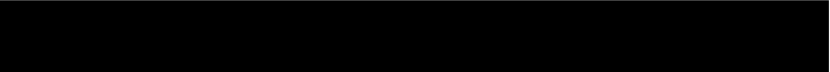
\includegraphics[width=1.2\paperwidth]{Logos/UCL page footer.png}
      }}
      

\thispagestyle{headings}
\maketitle
\FloatBarrier
\pagenumbering{roman}

\thispagestyle{empty}
% \begin{abstract}
%1.Talks about general application or general field of research
%2. Explains the challenge that is not answered yet
%3. Describe idea for tackling that challenge e.g. overall idea
%4 Methodology undertaken in research  e.g. tools, methods, steps taken.
%5. Main achievement of research supported by numerical results
%6. comparison with similar research in literature (qualitatively or quantitatively), and/or explain possible future applications of outcomes
\begin{abstract}
This project focuses on simulating qubit placement on physical devices and incorporating swap gates to address connectivity constraints in networked quantum computers. A key challenge in transpilation is the NP-hard problem of mapping logical qubits to physical qubits, particularly given the limited connectivity of physical qubits. This problem requires strategies for initial qubit placement and the insertion of swap gates when connectivity constraints are violated. The proposed approach utilizes physical qubit connectivity and gate priorities to generate an efficient initial mapping, followed by a dynamic lookahead window to insert swap gates more effectively. Although the Lookahead Swap method introduces slightly more swap gates than the default optimized Swap method, it significantly reduces circuit depth, making it very effective for noisy quantum hardware. In distributed quantum computing settings, layouts with higher connectivity perform better because of shorter distance between nodes, and organizing qubits into fewer groups further improves efficiency by simplifying information exchange and reducing circuit depth. This approach is particularly beneficial for networked quantum computers.
\\
\\
\\
\\
% \vspace{10pt}
\keywords{quantum computing - quantum circuit mapping - networked quantum computers}
\end{abstract}

% \newpage
% \thispagestyle{empty}
% \begin{center}
% I dedicate this ...
% \end{center}

% \newpage
% \thispagestyle{empty}
% \vspace*{\fill}
% \begin{center}
% Copyright \copyright  \thinspace 2022 by Joseph Rowell \\ All Rights Reserved
% \end{center}
% \vspace*{\fill}
% \newpage
% \thispagestyle{empty}
%\epigraph{The Book of Nature is written in the language of mathematics.}{--- \textup{Galileo Galilei}}
% \epigraph{The computer was born to solve problems that did not exist before.}{--- \textup{Bill Gates}}


\thispagestyle{empty}
\chapter*{Acknowledgements}

I would like to express my deepest gratitude to my supervisors, Abhishek Agarwal and Lachlan Lindoy, for their invaluable guidance, support, and encouragement throughout the development of this thesis. Their insight and expertise have been crucial to the successful completion of this project. I am also immensely grateful to Indonesia Endowment Fund for Education Agency (Lembaga Pengelola Dana Pendidikan), Ministry of Finance of Republic Indonesia for their full financial support throughout my master's study, which made this work possible. \\
I want to extend my heartfelt thanks to my family and friends for their unwavering support and understanding during this journey. Their patience and encouragement have been a constant source of strength. \\
Additionally, I would like to acknowledge IBM Qiskit team for providing the foundational framework that facilitated my research. As part of my contribution to this project, I developed and integrated transpilation algorithms, enhancing the overall functionality of the Qiskit software package, and I hope it will be beneficial to the quantum computing community.


\thispagestyle{empty}
\chapter*{Declaration}
I, Natasha Valentina Santoso, declare that the thesis has been composed by myself and that the work has not be submitted for any other degree or professional qualification. I confirm that the work submitted is my own. The report may be freely copied and distributed provided the source is explicitly acknowledged. \\
%Add signature png here.
\begin{figure}[H]

\includegraphics[width=0.3\linewidth]{Logos/signature.PNG}
\end{figure}
\vspace{-1em}
\noindent\begin{tabular}{ll}
Natasha Valentina Santoso & 22 August 2024 \\
\makebox[2.5in]{\hrulefill} & \makebox[2.5in]{\hrulefill}\\
\textit{Signature} & \textit{Date}\\
\end{tabular}



\tableofcontents

\thispagestyle{plain}
% \listoffigures
\listoftables
\listofalgorithms
\addcontentsline{toc}{chapter}{List of Algorithms}

% \printglossary[type=\acronymtype]
\printnoidxglossary[type=\acronymtype,title=Acronyms]

%%%%%%%%%%%%%%%%%%%%%%%%%%%%%%%%%%%%%%%%%%%%%%%%%%%%%%%%%%%%%%%%%%%%%%%%%%%%%%%%
% \chapter{Project Plan} \label{Chap1}


%%%%%%%%%%%%%%%%%%%%%%%%%%%%%%%%%%%%%%%%%%%%%%%%%%%%%%%%%%%%%%%%%%%%%%%%%%%%%%%%
% \pagenumbering{arabic}
\chapter{Introduction and Background} \label{Chap2}
\pagenumbering{arabic}

Quantum computers are expected to surpass classical computers in processing complex data, potentially revolutionizing various fields such as quantum chemistry \cite{Cao2019}, machine learning \cite{paler_machine_2023}, and quantum simulation \cite{peruzzo_variational_2014}. Currently, quantum computing is in the Noisy Intermediate-Scale Quantum (NISQ) era, characterized by quantum processors with tens to hundreds of qubits \cite{preskill_quantum_2018}. To expand the number of qubits, both academic and industrial efforts are shifting towards utilizing quantum networks to link multiple smaller quantum chips. However, significant challenges exist in connecting multiple quantum computers and executing circuits across them simultaneously, along with algorithmic difficulties due to device limitations. This project will focus on simulating qubit placement on physical devices and incorporating swap gates to address networked quantum computers connectivity constraints.

\section{Distributed Quantum Computing} % done chat, turnitin
\acrfull{dqc} involves breaking down a large quantum computation into smaller parts that are executed on multiple interconnected processors, rather than relying on a single large quantum computer with many qubits \cite{cuomo_towards_2020}. As shown in Figure \ref{fig:mono-vs-distributed}, this approach uses smaller quantum devices, each with a limited number of qubits, working together to perform complex computations. In this system, qubits can be shared and entangled between different quantum processors across a network, allowing the execution of quantum algorithms that require more resources than any single quantum processor could handle on its own. A primary goal in \acrshort{dqc} architecture is to minimize the number of operations, including connecting gates and interactions between different \acrfull{qpu} \cite{caleffi_distributed_2024}.
\begin{figure}[htb]
    \centering
    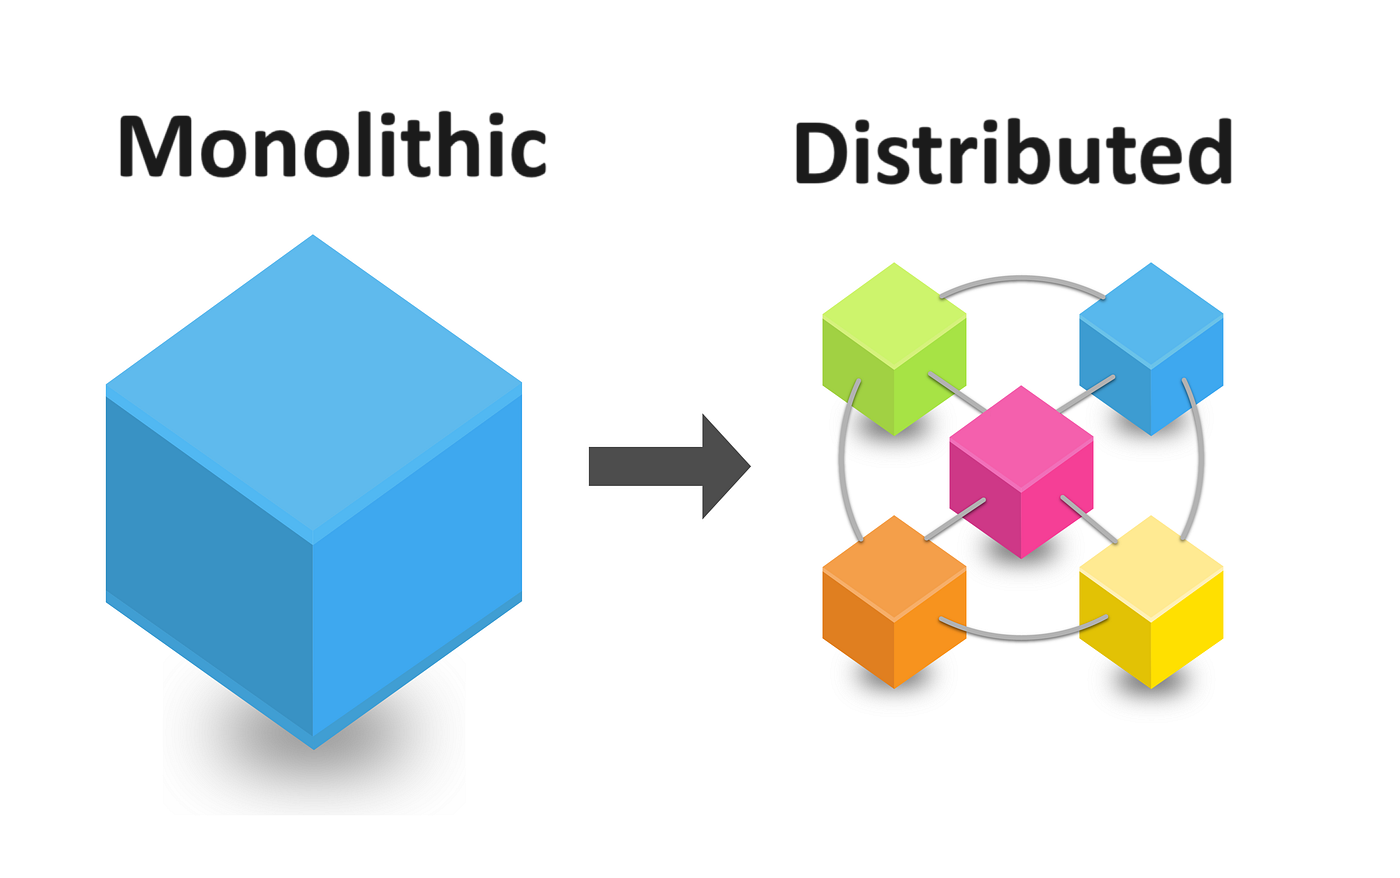
\includegraphics[width=0.4\linewidth]{image/mono vs distributed.png}
    \caption{Monolithic versus distributed illustration. Adapted from \cite{boroglu_microservices_2024}}
    \label{fig:mono-vs-distributed}
\end{figure}

\newpage
\section{Quantum Computing Architecture} % done chat, edited from turnitin, not yet checked for copy again
Gate-based quantum computing is the foundation of most quantum computing architectures today. These systems rely on a limited set of native quantum gates, including single-qubit gates (such as Pauli-X, Y, Z, Hadamard, and phase gates) and two-qubit gates like the Controlled-NOT (CNOT) gate.  While single-qubit gates can be applied directly to qubits, a CNOT gate requires the qubits to be adjacent on the coupling map. Despite the limited number of these gates, any quantum circuit can be constructed by carefully combining these operations \cite{barenco_elementary_1995}. This universality is a key aspect of quantum computing, enabling the design and execution of complex quantum algorithms within the constraints of available gate sets. \\
However, implementing these gates physically presents challenges, especially regarding qubit connectivity. In some quantum platforms, such as those using superconducting qubits \cite{krantz_quantum_2019}, the connectivity between qubits is constrained by the architecture's coupling graph. This graph defines the possible interactions between qubits, meaning not all qubits can directly interact with each other through two-qubit gates. As a result, additional operations, such as swap gates, may be needed to bring qubits into positions where the desired two-qubit gate can be applied. This added complexity can affect the efficiency and fidelity of quantum circuits, especially as the scale of the computation grows \cite{khandavilli_towards_2023}. \\
In this context, it is important to distinguish between logical qubits and physical qubits. According to \citeauthor{itoko_optimization_2020}, logical qubits refer to the abstract entities on which quantum algorithms and operations are defined (different from the concept of logical qubits in quantum error correction). These qubits exist independently of the physical hardware, representing the idealized qubits that are free from noise and hardware constraints. On the other hand, physical qubits are the actual qubits within a quantum processor where quantum operations are executed. The performance of physical qubits is influenced by hardware limitations such as decoherence, gate fidelity, and connectivity constraints \cite{itoko_optimization_2020}. Understanding the relationship between logical and physical qubits is crucial for effectively mapping quantum algorithms onto real quantum hardware, ensuring that the physical resources are used optimally while minimizing the effect of hardware imperfections. \\
In the 127-qubit IBM quantum system, \textit{ibm\_kyoto}, four single-qubit gates (ID, RZ, SX, X) and \acrshort{ecr} gates for two-qubit operations are supported. From Figure \ref{fig:ibm-kyoto}, a CNOT operation between $q_1$ and $q_2$ can be executed directly, but between $q_0$ and $q_2$, additional steps are needed. This highlights the requirement of a preliminary circuit preprocessing step, known as \textit{quantum transpiling} \cite{ferrari_compiler_2021}, before running a quantum circuit. \\
ircuit preprocessing step, known as \textit{quantum transpiling} \cite{ferrari_compiler_2021}, before running a quantum circuit. \\
\begin{figure}
    \centering
    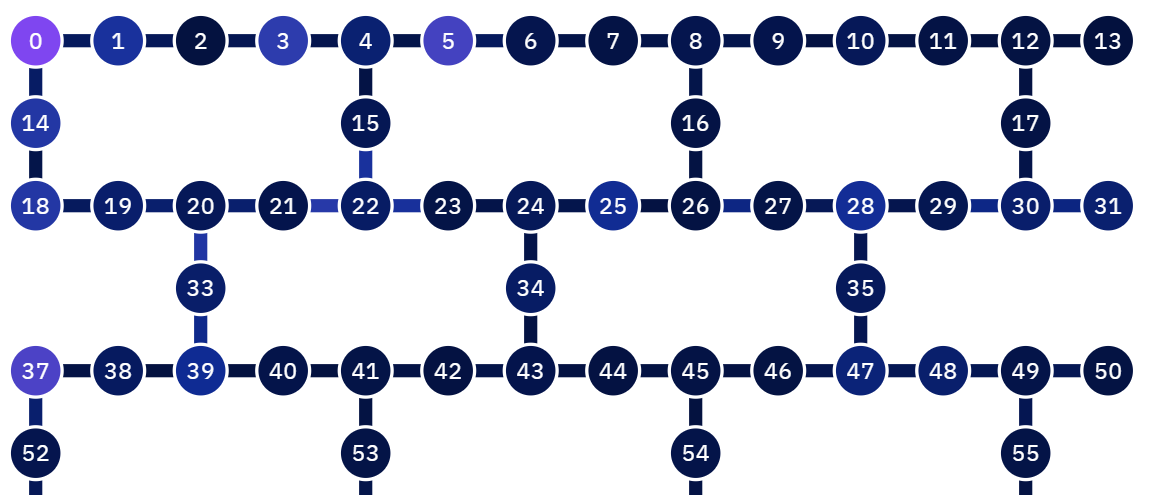
\includegraphics[width=0.6\linewidth]{image/ibm_kyoto.png}
    \caption{Partial coupling map of 127-qubit \textit{ibm\_kyoto}. Taken from \citeauthor{ibmquantum_computeresources} \protect\cite{ibmquantum_computeresources}. Each node represents a physical qubit, and the edges between nodes represent possible two-qubit gate operations}
    \label{fig:ibm-kyoto}
\end{figure}

\section{Quantum Circuit Mapping} % done chat, edited from turnitin not yet checked again
A quantum circuit compiler translates a logical quantum circuit into instructions that can be directly executed on a real \acrshort{qpu}. The compiler converts high-level programming languages, like Qiskit in Python \cite{aleksandrowicz_qiskit_2019}, into low-level instructions, such as OpenQASM \cite{cross_open_2017}. Quantum algorithms, as defined in quantum circuits, are generally hardware-agnostic and may not account for specific hardware limitations \cite{ash-saki_qure_2019}. to run these algorithms on a quantum processor, they must be adapted through a process called "quantum circuit mapping", which can increase gate count $(g)$ or circuit depth $(d)$, depending on the circuit and hardware constraints. \\
Figure \ref{fig:tackling-depth-gate-first} presents a 9-qubit device with two CNOT gates: $(q_1, q_2)$ (blue) and $(q_3, q_4)$ (green). The left side shows the original mapping and two different optimization approaches are explained:
\begin{enumerate}[nolistsep]
    \item \textbf{Depth First}: SWAP $(q_2, q_9)$, $(q_1, q_5)$ can be directly performed to connect CNOT $(q_1, q_2)$, and also SWAP $(q_4, q_8)$, $(q_3, q_7)$ to connect CNOT $(q_3, q_4)$. This method adds 4 SWAPs but only increases circuit depth by 1.
    \item \textbf{Gates First}: SWAP $(q_2, q_9)$ is done first, followed by swaps on $(q_2, q_3)$ and $(q_4, q_8)$. This method only adds 3 SWAPs but increases circuit depth by 2.
\end{enumerate} 
\begin{figure}[htb]
    \centering
    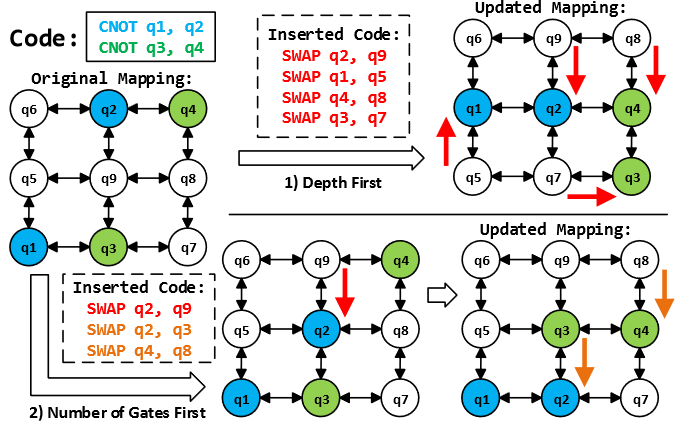
\includegraphics[width=0.6\linewidth]{image/tackling_depth_gate_first.png}
    \caption{Example of a trade-off between depth-first and gate-first. Adapted from \cite{li_tackling_2019}}
    \label{fig:tackling-depth-gate-first}
\end{figure}

\section{Qiskit Framework}
Qiskit is a quantum software program that converts quantum circuits into a format that can be executed on the IBM Quantum Platform \cite{ibmquantum_computeresources}. It utilizes a "transpilation" process to transform a given logical circuit to be compatible with a specific target device while also optimizing the circuit to enhance performance and achieve better results.

\subsection{Pass Manager}
The compilation process consists of six stages known as Pass Managers \cite{ibmquantum_transpiler} (Figure \ref{fig:transpiler}), which include:
\begin{enumerate}[nolistsep]
    \item \lstinline{init}: Runs initial passes to prepare the circuit for the backend, including unrolling custom instructions and converting multi-qubit gates into 1- and 2-qubit gates.
    \item \lstinline{layout}: Maps the logical qubits in the circuit to the physical qubits on the target quantum device.
    \item \lstinline{routing}: Inserts SWAP gates into the circuit to align with the physical connectivity of the backend, ensuring qubits that need to interact are adjacent.
    \item \lstinline{translation}: Converts the circuit's gates into the basis gates supported by the target backend, making the circuit executable on the specific hardware.
    \item \lstinline{optimization}: Performs multiple iterations of optimization to reduce circuit depth and gate count until a specified condition, such as a fixed depth, is met.
    \item \lstinline{scheduling}: Manages the timing and order of gate executions on the hardware to ensure optimal performance during execution.
    \begin{figure}[h]
        \centering
        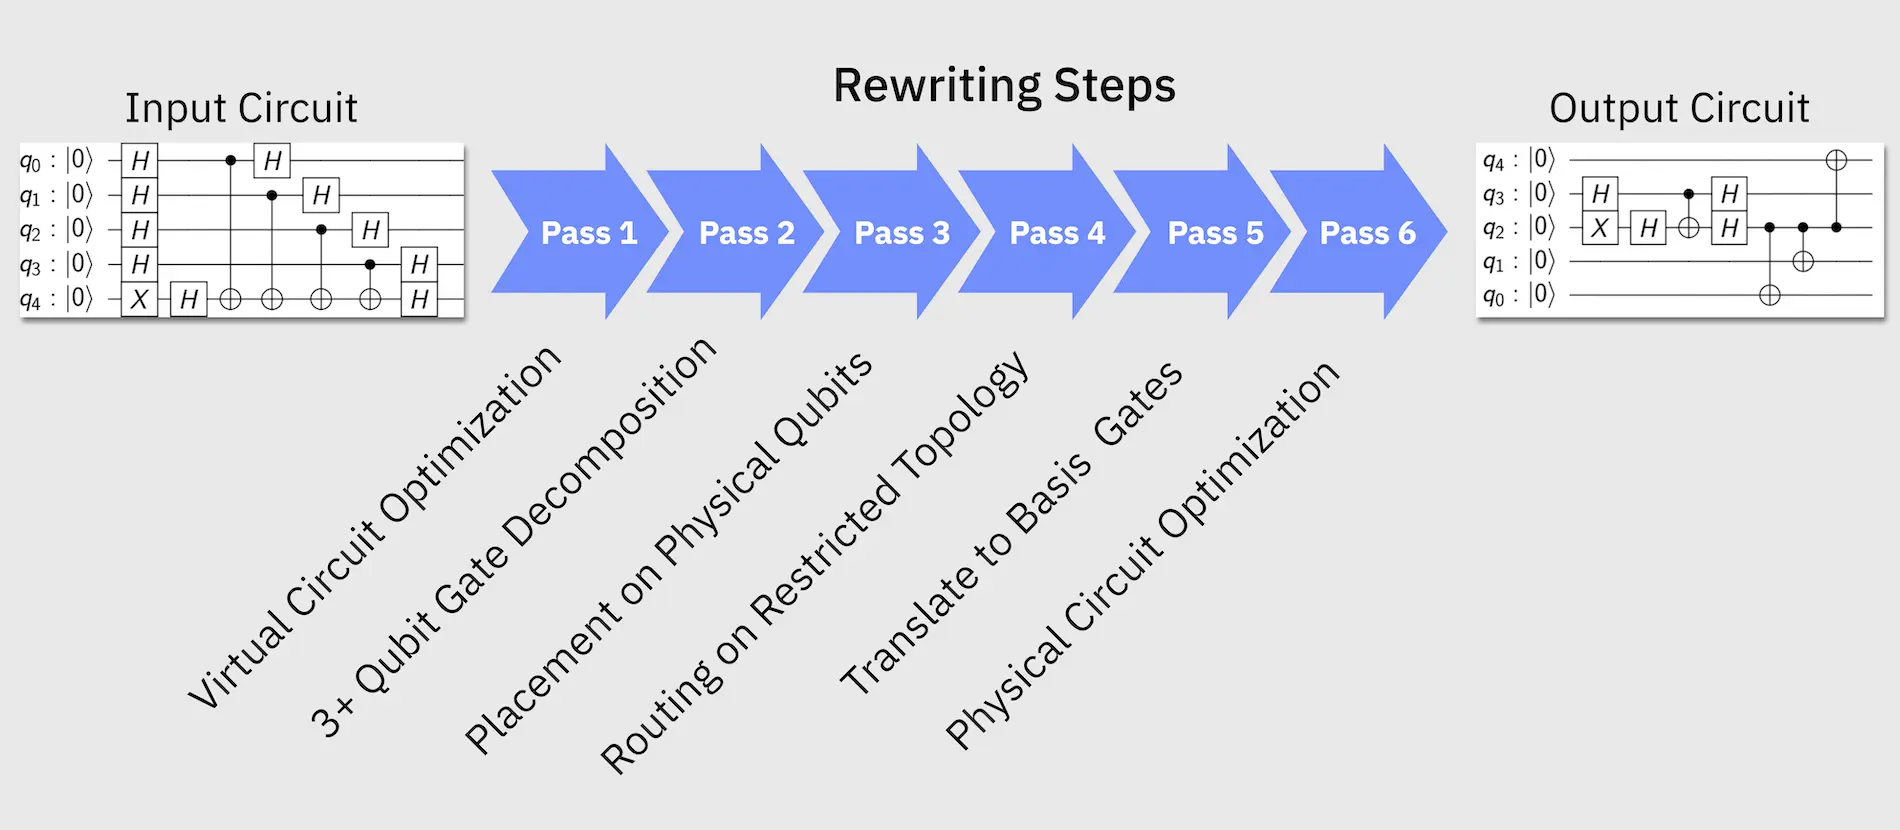
\includegraphics[width=0.75\linewidth]{image/transpiling_core_steps.png}
        \caption[Pass manager stages]{Pass manager stages. Adapted from \cite{ibmquantum_transpiler}}
        \label{fig:transpiler}
    \end{figure}
\end{enumerate}
This project will only focus on the first four stages until the translation stage.

\subsection{Initialization stage} % done chat, edited after turnitin, not yet checked
Most layout and routing algorithms only handle single- or two-qubit gates. Therefore, this stage unrolls any multi-qubit gates into sequences of single- or two-qubit gates, potentially increasing circuit size and depth \cite{ding_circuit_2020}. Two specific gates require decomposition by the backend:
\begin{enumerate}[nolistsep]
    \item A swap gate is decomposed into three CNOT gates, shown in Figure \ref{fig:swap-decompose}. While swap gates are essential for mapping a circuit onto the limited physical connectivity of a quantum device, they are expensive operations to execute on noisy quantum systems.
    \begin{figure}[h]
        \centering
        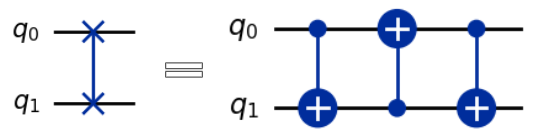
\includegraphics[width=0.5\linewidth]{image/swap decompose.png}
        \caption{Decomposed swap gate}
        \label{fig:swap-decompose}
    \end{figure}

    \item A Toffoli, also known as a controlled-controlled-not gate (CCX) gate, is a three-qubit operation. Since a Toffoli gate is not a native gate on most quantum hardware, it needs to be decomposed, typically using CNOT (controlled-NOT) gates and single-qubit operations, as illustrated in Figure \ref{fig:toffoli-decompose}. The standard decomposition of a Toffoli gate involves up to 6 CNOT gates and several single-qubit gates, such as Hadamard (H) and T-gates, making it a resource-intensive process.
    \begin{figure}[h]
        \centering
        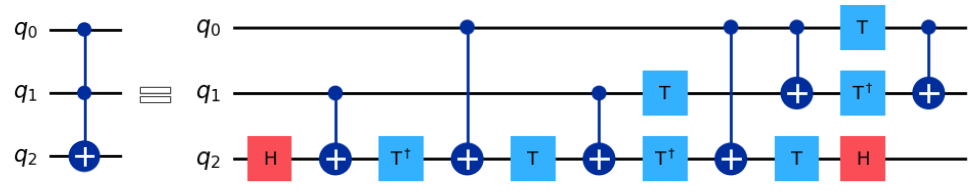
\includegraphics[width=0.5\linewidth]{image/toffoli decompose.png}
        \caption{Decomposed Toffoli gate}
        \label{fig:toffoli-decompose}
    \end{figure}
\end{enumerate}

\subsection{Layout Stage} % done chat, edited turnitin
Quantum circuits represent qubits used in computations, which must be directly mapped onto the physical qubits of a quantum device. Choosing the right initial layout is key to minimizing swap operations and reducing noise-related losses on physical qubits. This mapping, stored as a \lstinline{Layout} object, is a part of the constraints within a backend's \acrfull{isa}. For example, Figure \ref{fig:layout-placement} shows how a quantum circuit is mapped onto a device's coupling graph.
\begin{figure}[h]
    \centering
    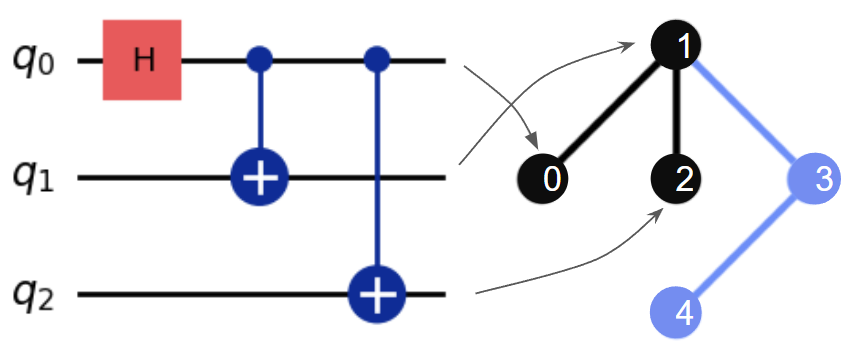
\includegraphics[width=0.5\linewidth]{image/layout_placement.png}
    \caption{Mapping logical qubits to physical qubits}
    \label{fig:layout-placement}
\end{figure}

\subsection{Routing Stage} % done chat, edited turnitin
The routing stage is a key part of the transpilation process that ensures two-qubit gates can be executed on a quantum device, considering its limited qubit connectivity. Since not all qubits on a device can interact directly, the routing stage adds SWAP gates to reposition qubits so that the required two-qubit operations are adjacent on the device's gate map \cite{wille_mqt_2023}, as shown in Figure \ref{fig:swap-placement}. Since swap gates are costly and introduce noise, minimizing their number is crucial. Qiskit uses a stochastic algorithm called \lstinline{SabreSwap} \cite{li_tackling_2019} to find an effective, though not always optimal, swap mapping. Because this method is stochastic, the resulting circuits can vary across runs, leading to different circuit depths and gate counts. \\
\begin{figure}[htb]
    \centering
    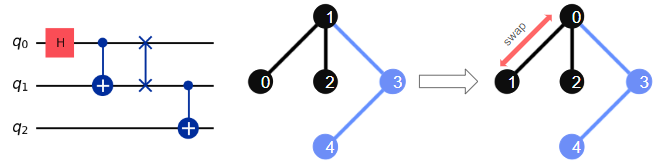
\includegraphics[width=0.7\linewidth]{image/swap_placement.png}
    \caption{Swap qubit states between physical $Q_0$ and and $Q_1$}
    \label{fig:swap-placement}
\end{figure}


\subsection{Translation Stage} % done chat, edited turnitin
When writing a quantum circuit, any arbitrary quantum gates can be used, including non-gate operations like qubit measurements and reset operations. Since most quantum devices only support a limited set of basic gates and non-gate operations, the quantum gates are translated into the native basis gates of a specific backend, which are part of the definition of a target's \acrshort{isa} \cite{gokhale_faster_2021}. For example, \lstinline{GenericBackendV2} class supports only a limited set of basic gates ['cx', 'id', 'rz', 'sx', 'x', 'reset', 'delay', 'measure'], while the quantum circuit (Figure \ref{fig:translation}) has $H$, $X$, and controlled-$P$ gates. After the transpilation process, a quantum circuit that initially had 5 logic gates is transformed into one with 12 gates.
\begin{figure}[htb]
    \centering
    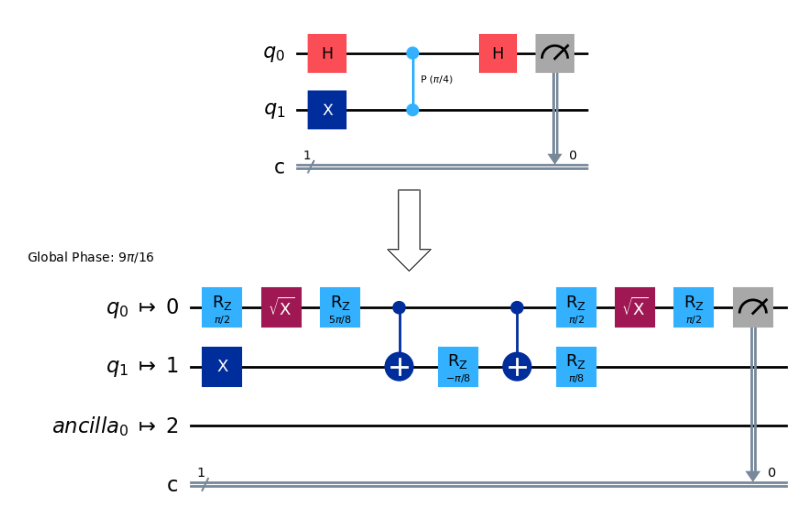
\includegraphics[width=0.7\linewidth]{image/translation_basis_gates.png}
    \caption{Translation basis gates}
    \label{fig:translation}
\end{figure}
% \pagenumbering{arabic}
%%%%%%%%%%%%%%%%%%%%%%%%%%%%%%%%%%%%%%%%%%%%%%%%%%%%%%%%%%%%%%%%%%%%%%%%%%%%%%%%
\chapter{Methodology} \label{Chap3}
One of the main challenges in transpilation is mapping logical qubits to physical qubits, especially since physical qubits often have limited connectivity. The qubit-mapping problem is classified as NP-hard \cite{botea_complexity_2021}, meaning that while optimal solutions may be achievable for small quantum circuits, the problem becomes increasingly difficult for larger circuits. Because most quantum hardware only allows two-qubit gates to operate between physically adjacent qubits, two important strategies are required: determining the initial placement of qubits and inserting swap gates when a gate execution violates these connectivity constraints \cite{cowtan_qubit_2019}.

For the overview of the algorithms, the initial step in addressing the qubit-mapping problem involves utilizing the physical qubit connectivity and gate priorities to generate an initial qubit mapping that is more efficient than a simple one-to-one layout. The subsequent step introduces a dynamic lookahead window to insert swap gates more efficiently taking into account gates that give positive effect to the swap candidate. This proposed algorithms successfully address the coupling limitations of quantum devices and reduce the overhead of inserting swap gates, leading to better performance on networked quantum hardware.

Table \ref{tab:definition-notation} provides the definitions for the notations used in the analysis:
\begin{table}[htb]
\centering
\caption{Definition of Notations}
\label{tab:definition-notation}
\begin{tabular}{|l|l|} 
\hline
\textbf{Notation} & \textbf{Definition}                                            \\ 
\hline
$n$               & number of logical qubits                                       \\ 
\hline
$q_{1,2,...,n}$     & logical qubits $q_L$ in quantum circuit                        \\ 
\hline
$N$               & number of physical qubits                                      \\ 
\hline
$Q_{1,2,...,N}$     & physical qubits $Q_P$ on quantum device                        \\ 
\hline
$C_{1,2,...,N}$     & classical register for quantum device                          \\ 
\hline
$g_i$             & number of gates in the circuit                                 \\ 
\hline
$d$               & depth of the circuit                                           \\ 
\hline
$G(V, E)$         & the coupling graph of the backend                              \\ 
\hline
$D[\ ][\ ]$       & the distance matrix of the physical qubits between $Q_i, Q_j$  \\ 
\hline
$\pi()$           & a mapping from $q_{1,2,...,n}$ to $Q_{1,2,...,N}$                  \\ 
\hline
$\pi^-1()$        & a mapping from $Q_{1,2,...,N}$ to $q_{1,2,...,n}$                  \\ 
\hline
$F$               & Front layer of quantum circuit                                 \\
\hline
\end{tabular}
\end{table}

\section{Layout}
% \cite{peham_optimal_2023} FOR LAYOUT RING STRUCTURE DST
\subsection{Distributed Coupling Graph} % done chat
Simulating a distributed quantum computer involves creating a coupling map that represents the connectivity of qubits across different "groups", with each group acting as a separate node or quantum processor within the quantum network. These groups consist of multiple \acrfull{qpu}, with connections both within each group and between different groups. The coupling graph defines the topology of the \acrshort{qpu} within each group, and this is managed using \lstinline{CouplingMap} \cite{ibmquantum_couplingmap} class in Qiskit. In this coupling graph, the last qubit of one group is connected to the first qubit of the next group, forming a larger distributed coupling map. By modifying the internal topology of a node (quantum computer) and the distribution of qubits across different groups, various configurations of the quantum network can be explored, as illustrated in Appendix \ref{app:coupling-graph-by-group}. \\
The following functions are used to define the topology within each group:
\begin{itemize}[nolistsep]
    \item \lstinline{from_line}: creates a coupling map of $n$ qubits connected in a line.
    \item \lstinline{from_grid}: creates a coupling map of qubits arranged in a grid with a specified number of rows and columns.
    \item \lstinline{from_ring}: creates a coupling map of $n$ qubits connected in a ring.
    \item \lstinline{from_full}: creates a fully connected coupling map on $n$ qubits.
    \item \lstinline{from_t_horizontal}: creates a coupling map of five qubits arranged in a T-shape, connected at the longer end.
    \item \lstinline{from_t_vertical}: creates a coupling map of five qubits arranged in a T-shape, connected at the shorter end.
\end{itemize}

\subsection{Interaction Mapping} % done chat
In this section, an algorithm called \mycode{InteractionLayoutMapping} will be discussed to determine the most appropriate mapping from logical qubits to physical qubits. During the initialization step, the connectivity of the physical qubits on the backend is determined, and the priority of two-qubit gates is assigned based on their order of appearance in the quantum circuit, with gates appearing earlier (on the left side) being given higher priority \cite{liu_qm-dla_2024}. Additionally, a metric is calculated to measure qubit interactions that quantify how qubits interact with each other within a circuit, particularly on how qubits are connected through multi-qubit gates, such as CNOT gates \cite{bandic_interaction_2023}. This calculation will help to define the order in which quantum gates are prioritized.

\begin{definition} % done chat
    Physical connectivity is the number of neighbours of physical qubits ($Q_P$).
\end{definition}
A physical quantum device is represented by a coupling graph, which is a directed graph (V, E). In this graph, $Q = \{Q_0, Q_1, ..., Q_{N-1}\}$ represents the set of physical qubits as vertices (V), and the edges (E) represent the direct connections between two physical qubits, $Q_i$ and $Q_j$, where a two-qubit gate can be applied. When a physical qubit has higher connectivity, the logical qubit mapped to it has a greater chance of connecting to other logical qubits without needing additional swap gates. Conversely, if a physical qubit has low connectivity, more qubit movements will be needed to satisfy the coupling constraints before a logical gate can be operated. These additional movements increase the need for swap gate insertions, leading to a larger circuit size and depth, which may negatively impact gate fidelity and runtime. For example, Qiskit \lstinline{FakeLondonV2} \cite{ibmquantum_fakelondonv2} (Figure \ref{fig:fake-london})  is a simulated 5-qubit backend with a coupling graph that illustrates the physical connectivity on each qubit.
\begin{figure}[h]
    \centering
    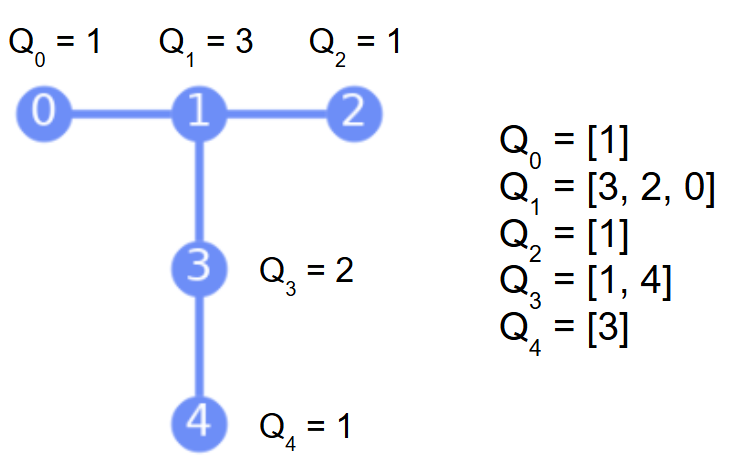
\includegraphics[width=0.5\linewidth]{image/fake_london.png}
    \caption{\lstinline{FakeLondonV2} coupling map and its physical connectivity list containing the number of neighbours of each physical qubit $Q_P$.}
    \label{fig:fake-london}
\end{figure}

\begin{definition} % done chat
    Logical priority calculates the number of two-qubit gates acting on each logical qubit in a quantum circuit.
\end{definition}
If two logical qubits have the same priority value, the one with the earlier index is given precedence. The logical neighbours list identifies other logical qubits that interact with a specific logical qubit $q_i$ in the circuit. Figure \ref{fig:logical-priority} lists the number two-qubit gates operating on the wire of the quantum circuit.
\begin{figure}[h]
    \centering
    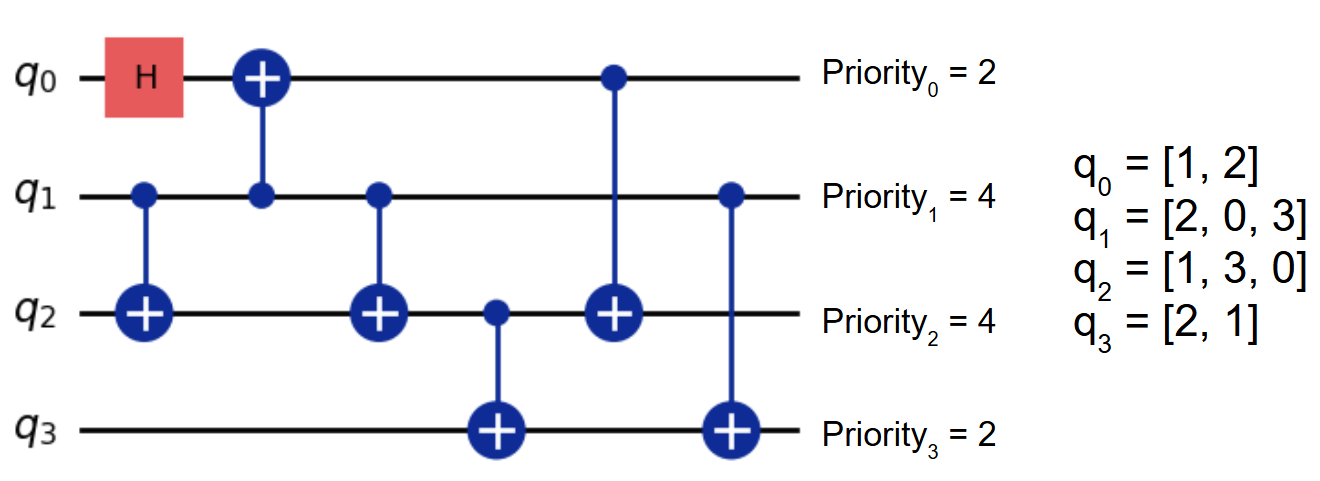
\includegraphics[width=0.7\linewidth]{image/logical_priority.png}
    \caption{Logical priority of a quantum circuit and its logical neighbours list containing the indices of qubits that interact with the logical qubit $q_i$.}
    \label{fig:logical-priority}
\end{figure}

\begin{definition} % done chat
    Gate weight reflects the importance of each gate $g_i$ in a quantum circuit, based on when it occurs in the sequence of operations.
\end{definition}
In a quantum circuit, consider a set of logical qubits $q_L = \{q_0, q_1, ..., q_{n-1}\}$ and an ordered sequence of gates $g = \{g_0, g_1, ..., g_{m-1}\}$. It is important to note that the ordering of gates introduces some arbitrariness, as certain gates can be implemented in parallel. For example, the last two gates in Figure \ref{fig:gate-weight}, CNOT $(q_0, q_2)$ and CNOT $(q_1, q_3)$, could be executed simulatenously, making the weights of $g_6$ and $g_7$ interchangeable. \\
Each quantum gate $g_i$ is assigned a weight $w_i$, which is calculated as:
\begin{equation}
    w_i = m - i
\end{equation}
where $m$ is the total number of gates in the quantum circuit, and $i$ is the gate's position in the sequence. A higher weight suggests that the gate occurs earlier in the sequence, potentially having a greater influence on the subsequent operations and the final state of the quantum system. Figure \ref{fig:gate-weight} shows the gate weights in descending order, with earlier gates assigned higher values.
\begin{figure}[h]
    \centering
    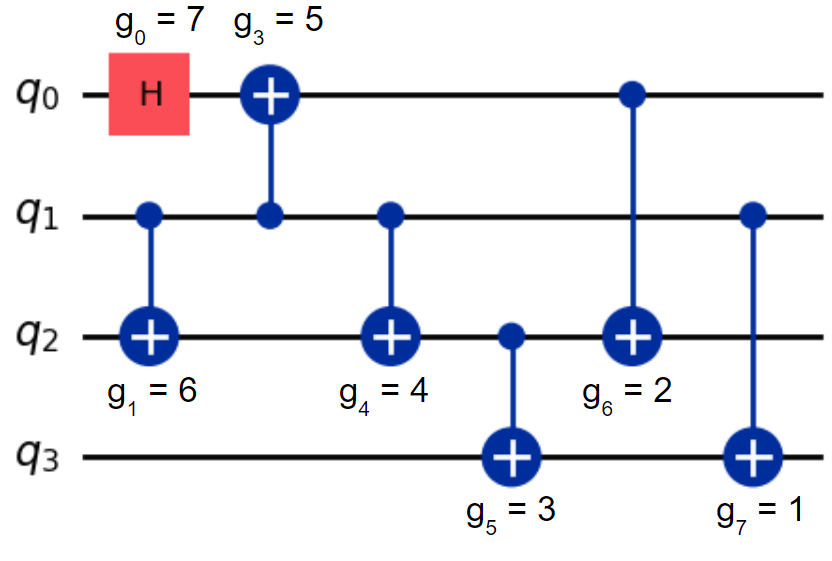
\includegraphics[width=0.4\linewidth]{image/gate_weight.png}
    \caption{Gate weight of a quantum circuit, with front gates assigned higher weights}
    \label{fig:gate-weight}
\end{figure}

\begin{definition}
    \acrfull{qpi} refers to the measure of interaction logical qubit pair (q\textsubscript{i}, q\textsubscript{j}) when they are involved in a multi-qubit quantum gate, such as controlled-NOT (CNOT) gate or any other two-qubit gate.
\end{definition}
\acrshort{qpi} is determined by summing all gate weights that involve the qubit pair and is represented as a 2D matrix, as in Table \ref{tab:qpi-matrix}:
\begin{equation}
    \text{QPI}(q_i, q_j) = \sum_{k \in \mathcal{G}(q_i, q_j)} w_k
\end{equation}
where $\mathcal{G}(q_i, q_j)$ represents the set of indices $k$ corresponding to gates that involve both qubits $q_i$ and $q_j$, and $w_k$ is the weight of gate $g_k$. \\
\begin{table}[h]
    \centering
    \begin{tabular}{|c|c|c|c|c|c|}
        \hline
        $(q_i, q_j)$ & (0, 1) & (0, 2) & (1, 2) & (1, 3) & (2, 3) \\
        \hline
        QPI & 5 & 2 & 10 & 1 & 3 \\
        \hline
    \end{tabular}
    \caption{\acrshort{qpi} value of gates on logical qubits $(q_i, q_j)$ from quantum circuit on Figure \ref{fig:gate-weight}.}
    \label{tab:qpi-matrix}
\end{table}

\begin{definition}
    \acrfull{qbn} refers to the sum of weights of the qubit pairs interactions (\acrshort{qpi} values) that involve the logical qubit being considered and its neighbouring physical qubits.
\end{definition}
A higher \acrshort{qbn} value indicates that the qubit is more connected or plays a more significant role within the quantum circuit. The \acrshort{qbn} value is defined as:
\begin{equation}
    \text{QBN}(q_i) = \sum_{j} \text{QPI}(q_i, Q_{P,j})
\end{equation}
where $q_i$ is the logical qubit under consideration, $Q_{P,j}$ denotes each physical qubit that is adjacent to or interacts with $q_i$, and $\text{QPI}(q_i, Q_{P,j})$ represents the interaction strength (weight) between $q_i$ and the $j$-th adjacent physical qubit.

\subsection{Interaction Mapping Algorithm}
Algorithm \ref{alg:interaction-layout-mapping} \mycode{InteractionLayoutMapping} outlines the steps for creating an initial qubit mapping, where the inputs are the device's coupling map and the circuit's \acrfull{dag}, and the output is a layout that maps logical qubits $(q_L)$ to physical qubits $(Q_P)$. The algorithm starts by calculating physical connectivity from the coupling map and determining the logical qubits' priorities, which are sorted in descending order. The logical qubit with the highest priority is then mapped to the physical qubit with the most connections. For subsequent placements, the algorithm checks if the assigned physical qubits have adjacent neighbours. If they do, it evaluates \acrfull{qpi} between the logical neighbours and their corresponding qubits, selecting the highest QPI candidate for mapping. If no adjacent neighbours meet this criterion, the algorithm assigns the next highest physically connected qubits to the logical qubits. This process generates all possible mappings for the quantum circuit, which are then ranked based on their total QPI index, and the final output is one initial mapping with the highest QPI rank. If multiple mappings have the same top QPI rank, the final output may be different with each run.

\begin{algorithm}[htb]
\caption{Interaction Layout Mapping}\label{alg:interaction-layout-mapping}
\hspace*{\algorithmicindent} \textbf{Input} Coupling Graph G(V, E), Circuit DAG \\
\begin{algorithmic}[1]
\State physical connectivity $\gets E$ on $Q_P$
\State logical priority $\gets g$ on $q_L$
\If{coupling graph is mostly fully connected}
\State \Return one-to-one index mapping
\EndIf
\State maps = [\ ]
\While{logical priority is not empty}
    \For{maps}
        \State $q_i \gets$ max (logical priority)
        \State temp physical connectivity $\gets$ neighbours of assigned $Q_P$
        \If{all $q_i$ neighbours already assigned}
            \State $Q_X \gets$ max(temp physical connectivity)
            \State maps $\gets (q_i, Q_X)$
        \Else
            \State $Q_X$ neighbours[\ ] $\gets$ adjacent assigned $Q_P$
            \State Get all assigned $q_L$ from maps
            \For{available $Q_X$ neighbours}
                \State $q_j \gets \pi^{-1}(\text{available }Q_X)$
                \State QBN candidate $\gets \text{QPI}[q_i][q_j]$
            \EndFor
            \State $Q_X \gets$ max (QBN value)
            \State maps $\gets (q_i, Q_X)$
        \EndIf
    \EndFor
\EndWhile
\end{algorithmic}
\end{algorithm}

\begin{example} % done chat
The initial quantum circuit shown in Figure \ref{fig:circuit-init} is processed through Algorithm \ref{alg:interaction-layout-mapping} \mycode{InteractionLayoutMapping} to obtain a more efficient solution for qubit placement. The backend device used is a simulated five-qubit system, \lstinline{FakeLondonV2}. \\
First, logical qubit $q_1$ is directly assigned to $Q_1$, which has the most connections with three neighbours. The current mapping is $[[\colorbox{backcolour}{(1, 1)}]]$, where the first value in the tuple represents the logical qubit $(q_L)$ and the second value represents the physical qubit $(Q_P)$. Next, logical qubit $q_2$ is to be assigned to the available physical candidates $Q_3$, $Q_2$, and $Q_0$. The \acrshort{qpi}$(q_1, q_2)$ value is 10 for all these candidates, so they are all included in the mapping. The current mapping is $[[(1, 1), \colorbox{backcolour}{(2, 3)}], [(1, 1), (2, 2)], [(1, 1), (2, 0)]]$, and the sum of \acrshort{qbn} is recorded. Figure \ref{fig:circuit-mapping} illustrates the path when physical qubit $Q_3$ is chosen for logical qubit $q_2$. The next logical qubit, $q_0$, has possible physical candidates $Q_0$, $Q_2$, and $Q_4$. Using the mapped logical qubits and their assigned physical qubits, the \acrshort{qpi} values are calculated, and the \acrshort{qbn} values are summed to determine the maximum value. For the neighbour of $Q_1$, the \acrshort{qpi} between $q_0$ and $q_1$ is 5, while for the neighbor of $Q_3$, the \acrshort{qpi} between $q_0$, $q_2$ is 2. The maximum value occurs for both $Q_0$ and $Q_2$. Therefore, the updated mapping for path $[(1, 1), (2, 3)]$ is $[[(1, 1), (2, 3), \colorbox{backcolour}{(0, 2)}], [(1, 1), (2, 3), (0, 0)]]$. With the last mapping of $(q_0, Q_2)$, the last logical qubit is for $q_3$ has available candidates $Q_0$ and $Q_4$. If $q_3$ is assigned to $Q_0$, the \acrshort{qpi} value is 1, while for $Q_4$, the \acrshort{qpi} value is 3. The final assignment is $(q_3, Q_4)$ and \acrshort{qbn} rank is updated accordingly. The algorithm not only generates all possible paths for mapping but also identifies the path with the highest \acrshort{qbn} rank. The chosen layout is $[(1, 1), (2, 3), (0, 0), \colorbox{backcolour}{(3, 4)}]$, as shown in Figure \ref{fig:plot-circuit-layout}, with a total rank of $18.0$. The initial quantum circuit is redrawn as in Figure \ref{fig:circuit-layout-isa}.
\end{example}

\begin{figure}[htbp]
    \centering
        \begin{subfigure}{0.6\linewidth}
        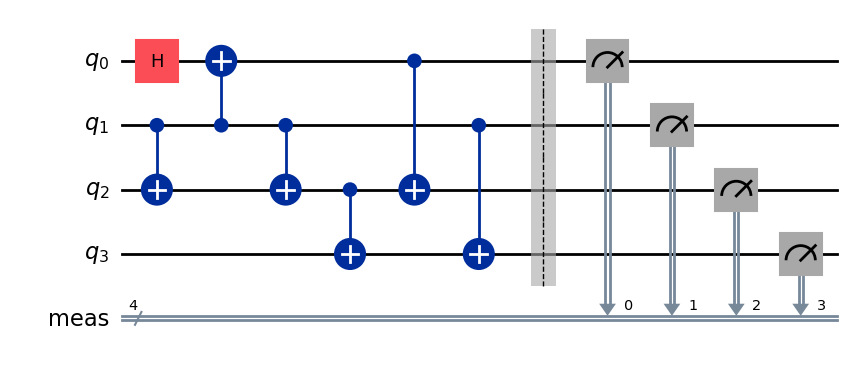
\includegraphics[width=\linewidth]{image/circuit_init.png}
        \caption{Initial quantum circuit}
        \label{fig:circuit-init}
    \end{subfigure}
    \vspace{1em}
    \begin{subfigure}{0.8\linewidth}
        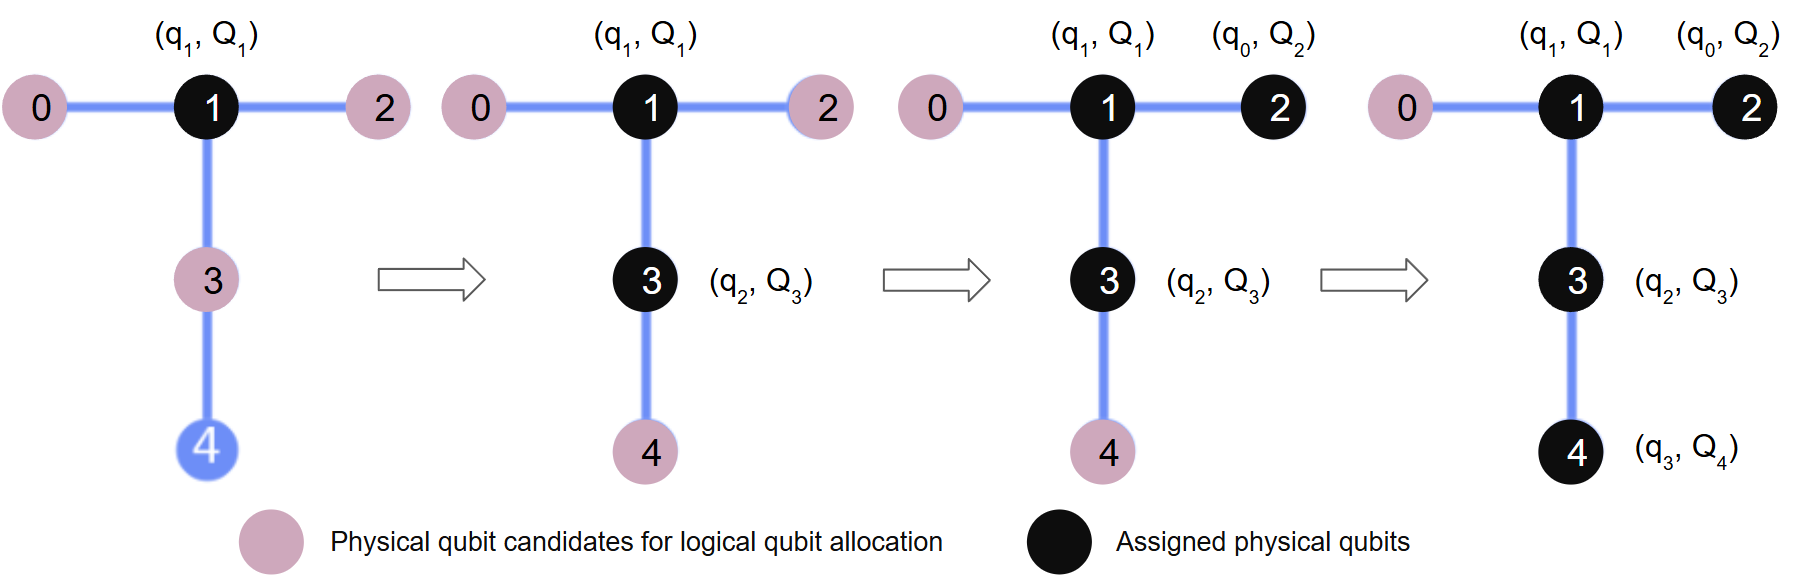
\includegraphics[width=\linewidth]{image/circuit_mapping.png}
        \caption{Steps to assign logical qubit to backend coupling map}
        \label{fig:circuit-mapping}
    \end{subfigure}
    \vspace{1em}
    \begin{subfigure}{0.6\linewidth}
        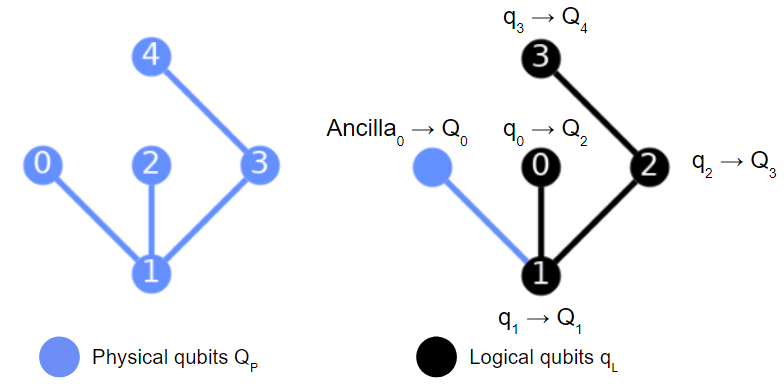
\includegraphics[width=\linewidth]{image/plot_circuit_layout.png}
        \caption{$\pi(q_L, Q_P)$ mapping in the coupling map, where the blue nodes on the left are physical qubits $Q_P$, and the black nodes on the right are logical qubits $q_L$ assigned to the physical qubits.}
        \label{fig:plot-circuit-layout}
    \end{subfigure}
    \vspace{1em}
    \begin{subfigure}{0.6\linewidth}
        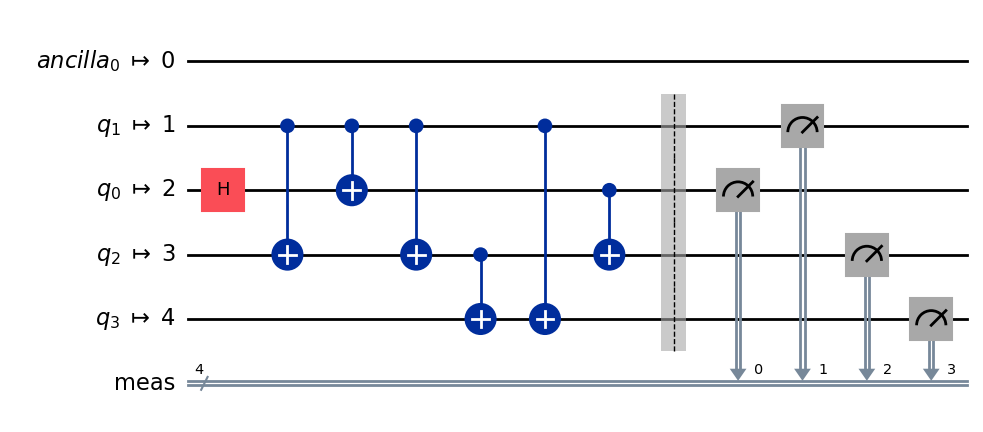
\includegraphics[width=\linewidth]{image/circuit_layout.png}
        \caption{Redraw quantum circuit in embed coupling map}
        \label{fig:circuit-layout-isa}
    \end{subfigure}
    \caption{Interaction layout mapping $(q_L, Q_P)$}
\end{figure}

\subsection{Analysis Pass} % done chat
Qiskit framework provides specific \lstinline{AnalysisPass} \cite{ibmquantum_analysispass} to change the property set of a quantum circuit. The custom analysis pass requires layout mapping as input, builds the mapping to Qiskit \lstinline{Layout} \cite{ibmquantum_layout} class, and implements the abstract run function. The class layout constructs a bijective dictionary, mapping virtual qubits $q_L$ to physical qubits $Q_P$. An AnalysisPass might be used to evaluate the effectiveness of a given qubit layout, guiding the optimization process and ensuring that the final circuit is well-suited for the physical quantum hardware it will run on.

\newpage
\section{Routing}
\subsection{Lookahead Swap}
When addressing the qubit mapping problem, all two-qubit gates must meet the hardware connectivity constraints. Single-qubit gates, which act on individual physical qubits, are not relevant and can be ignored for the mapping problem. In most cases, it is not feasible to find a mapping that satisfies all connectivity constraints for the entire quantum circuit. Therefore, whenever a gate does not meet these constraints, the mapping between logical and physical qubits must be updated using swap gates. However, adding swap gates can greatly affect the order of subsequent logical gates. The main metrics for evaluating these adjustments are the number of additional swap gates needed and the resulting circuit depth.

% from chat
\begin{definition}
    DAGCircuit \cite{ibmquantum_dagcircuit} is a \acrfull{dag} representation of a quantum circuit. This intermediate representation allows the manipulation and optimization of quantum circuits.
\end{definition}
In the \acrshort{dag}, each node corresponds to a quantum gate or a measurement applied to qubits, while the edges indicate the flow of quantum information between operations, connecting the output of one operation to the input of another. The \acrshort{dag} structure can be analysed by counting the number of qubits and assessing the circuit depth, which may help simplify the circuit by merging gates, eliminating redundant operations, and applying other techniques to reduce the circuit's complexity \cite{li_tackling_2019}. Figure \ref{fig:dag-embeded} illustrates the flow of a quantum circuit, where green nodes represent logical qubit inputs, blue nodes represent logical gates $g$, and red nodes represent logical qubit outputs. The edges in the graph depict the quantum information flow from input to output. Additionally, each level in the graph corresponds to the quantum circuit depth, so when multiple nodes appear at the same level, it indicates that the gate operations are applied to disjoint physical qubits.
\begin{figure}[h]
    \centering
    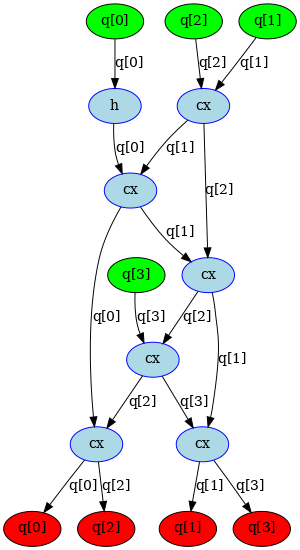
\includegraphics[width=0.3\linewidth]{image/dag_embeded.png}
    \caption{\acrfull{dag} of the previous quantum circuit (Figure \ref{fig:circuit-init}). \acrshort{dag} consists of three nodes: \acrshort{dag} input nodes (green), \acrshort{dag} operation nodes (blue), and \acrshort{dag} output nodes (red). The arrows indicate the quantum information flow.}
    \label{fig:dag-embeded}
\end{figure}

\begin{definition}
    The Gate Front Layer refers to a series of quantum gates that have no pending predecessors on their associated qubits.
\end{definition}
A layer in a quantum circuit consists of gates that operate on non-overlapping qubits, and the total number of layers corresponds to the circuit depth, denoted as \textit{d}. From Qiskit documentation, these layers are generated using a greedy algorithm. The resulting layer includes new \acrshort{dag} operation nodes, \acrshort{dag} input nodes, and \acrshort{dag} output nodes. In the \acrshort{dag} illustrated in Figure \ref{fig:dag-embeded}, the front layer consists of the $CX$ and $H$ gates.

\begin{definition} % done chat
    Nearest neighbour distance refers to the shortest distance between a given qubit and its closest neighbouring qubit in a quantum device. 
\end{definition}
In most quantum hardware, two-qubit gates (like CNOT or CZ gates) can only be directly implemented between qubits that are physically adjacent. If the two qubits involved in the gate are not neighbours, they need to be moved closer together through a series of SWAP operations, which exchange the positions of qubits on the device. \\
In the setup Figure \ref{fig:nearest-neighbour-distance}, the nearest neighbour distance between $Q_0$ and $Q_1$ is 1, the nearest neighbour distance between $Q_1$ and $Q_2$ is 1, and the nearest neighbour distance between $Q_0$ and $Q_2$ is 2, as they are not direct neighbours.
\begin{figure}[htb]
    \centering
    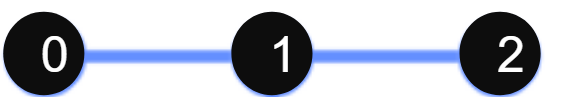
\includegraphics[width=0.25\linewidth]{image/nearest_neighbour_distance.png}
    \caption{Example of nearest neighbour distance setup, where distance $Q_0 - Q_1$ is 1, and distance $Q_0 - Q_2$ is 2.}
    \label{fig:nearest-neighbour-distance}
\end{figure}

\begin{definition} % done chat
    The dependency list for $q_i$ contains the quantum gates $g_i$ that are located at logical qubits $q_L$. This list only considers two-qubit gates.
\end{definition}
The dependency list starts with the front layer of quantum gates that have no preceding gates, which is the leftmost gate in each dependency list\textsubscript{i}. A two-qubit gate is included in two related dependency lists and becomes an active gate when it is the front gate for both associated logical qubits at the same time. As shown in Figure \ref{fig:dependency-list}, gate $g_1$, as the front gate for both dlist\textsubscript{1} and dlist\textsubscript{3}, makes it an active gate. Single-qubit gates are not included in the dependency list because they can be directly executed on a physical qubit without requiring special consideration.
\begin{figure}[htbp]
    \centering
    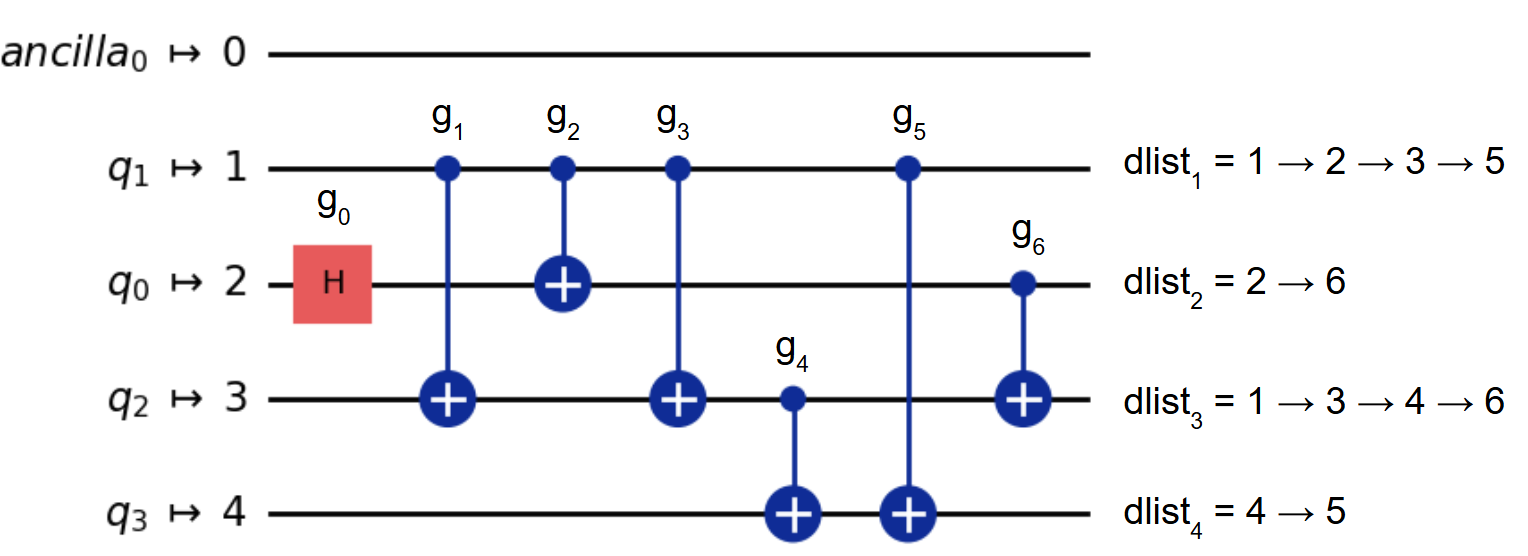
\includegraphics[width=0.7\linewidth]{image/dependency_list.png}
    \caption{The dependency list of a quantum circuit, where dlist\textsubscript{1} contains $g_1, g_2, g_3, \text{and } g_5$, which are two-qubit gates that lie on $q_1$.}
    \label{fig:dependency-list}
\end{figure}

\begin{definition} % done chat
    The effect of a swap gate on a specific two-qubit gate is defined as the change in the nearest neighbour distance of that gate before and after the swap is applied.
\end{definition}
When a swap gate is applied, it alters the nearest neighbour distance for subsequent two-qubit gates that share a logical qubit with the swap. Each swap impacts only one distance, leading to one of three outcomes: the distance can decrease by 1 (positive effect), increase by 1 (negative effect), or remain unchanged (no effect) \cite{zhu_dynamic_2020}. In figure \ref{fig:lookahead-window}, each rectangle represents a two-qubit gate, with $``+"$ indicates a non-negative effect (0 or +1), while $``-"$ signifies a negative effect (-1).

\begin{figure}[h]
    \centering
    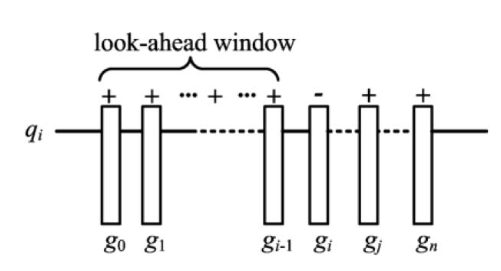
\includegraphics[width=0.5\linewidth]{image/lookahead_window.png}
    \caption{Diagram for the dynamic look-ahead technique. Adapted from \cite{zhu_dynamic_2020}}
    \label{fig:lookahead-window}
\end{figure}

The effect of a swap gate applied to $(Q_i, Q_j)$ changes the nearest neighbour distance of $g_i$, as determined by the logical to physical mapping before the swap $(\pi_1)$ and after the swap $(\pi_2)$.
\begin{equation}
    \text{effect}(\text{SWAP}, g_i) = \text{dist}(g_i, \pi_1) - \text{dist}(g_i, \pi_2)
\end{equation}

\begin{definition}
    The look-ahead technique is a heuristic cost function used to evaluate how effectively a swap gate ensures that the circuit meets connectivity constraints.
\end{definition}
The method used in Qiskit relies on a fixed window size that is determined before the mapping process begins \cite{ibmquantum_lookaheadswap}. This fixed window approach has limitations because it considers a predetermined number of gates across all qubits, regardless of their relevance. Additionally, with a fixed-size window, the heuristic cost function might select a swap gate that helps some gates scheduled later but negatively impacts those that are executed earlier. In extreme cases, the chosen swap could be harmful to current active gates but may be beneficial for future ones, potentially slowing down or even blocking the heuristic algorithm to progress. \\
To overcome these issues, a dynamic look-ahead technique is introduced as the heuristic cost function. This approach evaluates the effect of a swap gate by focusing only on the two-qubit gates directly affected by the swap. It selectively looks ahead at the two logical qubits ($q_i$ and $q_j$) that experience a positive effect, stopping when a negative effect is encountered. As illustrated in Figure \ref{fig:lookahead-window}, lookahead window only considers from $g_0$ to $g_{i-1}$, where the values are non-negative. The look-ahead window sums all the non-negative (1 or 0) effects on the logical qubit $q_L$:
\begin{equation}
    \text{Lookahead}(\text{SWAP}, q_i) = \sum_{g \in \text{window}} \text{effect}(g)
\end{equation}
The value of Lookahead(SWAP) includes both logical qubits $q_i$ and $q_j$ where the swap gate is inserted,
\begin{equation}
    \text{Lookahead}(\text{SWAP}) = \text{Lookahead}(\text{SWAP}, q_i) + \text{Lookahead}(\text{SWAP}, q_j)
\end{equation}
All these definitions are incorporated to Algorithm \ref{alg:lookahead-swap-routing} \mycode{Lookahead Swap Routing}.
\begin{algorithm}[htbp]
\caption{Lookahead Swap Routing}\label{alg:lookahead-swap-routing}
\hspace*{\algorithmicindent} \textbf{Input} Coupling Graph G(V, E), Circuit DAG \\
\hspace*{\algorithmicindent} \textbf{Output} Circuit DAG
\begin{algorithmic}[1]

\Procedure{check gate connectivity}{$g_i$}
    \State $Q_i \gets \pi(q_i)$
    \State $Q_j \gets \pi(q_j)$
    \State $D[Q_i][Q_j]$
    \If{$D[Q_i][Q_j] == 1$}
        \State dlist[$q_i$] pop front
        \State dlist[$q_j$] pop front
        \State new\_dag apply operation back($g_i$)
    \Else
        \State act\_list.append($g_i$)
    \EndIf
\EndProcedure

\item[]

\State dlist[\ ] $\gets$ $g_i$ on $q_n$ iff two-qubit gates
\State new\_dag $=$ dag.copy\_empty()
\State act\_list $= [\ ]$
\For{dag layers} \Comment{traverse circuit depth per level}
    \For{$g_i$ in dag operation nodes}
        \If{$g_i$ is a two-qubit gate of ($q_i, q_j$)}
            \State check gate connectivity($g_i$)
        \Else
            \If{$g_i$ is 'measure' operation}
                \State $C_i \gets q_i$ the corresponding updated $Q_P$ for register
            \EndIf
            \State new\_dag apply operation back($g_i$)    
        \EndIf
    \EndFor
    \While{act\_list is not empty}
        \State check gate connectivity($g_i$)
        \State candidate list $=$ generate possible physical swaps
        \For{swap$(Q_x, Q_y)$  in candidate list}
            \State Lookahead $(\text{swap}(Q_x, Q_y)) = \sum_{g} \text{effect}(Q_x(g)) + \sum_{g} \text{effect}(Q_y(g))$
        \EndFor
        \State highest swap $(Q_x, Q_y)$ $\gets$ max(lookahead)
        \State new\_dag apply operation back(SwapGate$(Q_x, Q_y)$)
    \EndWhile
\EndFor
\end{algorithmic}
\end{algorithm}

\subsection{Lookahead Swap Routing Algorithm}
Figure \ref{fig:swap-trivial-basic} demonstrates the transpilation process using Qiskit \lstinline{TrivialLayout} \cite{ibmquantum_triviallayout} and \lstinline{BasicSwap} \cite{ibmquantum_basicswap} routing methods. The \lstinline{TrivialLayout} assigns virtual qubits to physical qubits by mapping $n$ logical qubits to device qubits $0, 1, ...,, N-1$ in ascending order. The \lstinline{BasicSwap} then performs minimal adjustments by inserting one or more swap gates before a two-qubit gate until the quantum information is located at adjacent physical qubits. \\
In contrast, Figure \ref{fig:swap-lookahead} illustrates the process using the interaction layout from Algorithm \ref{alg:interaction-layout-mapping}. Initially, the algorithm converts the circuit to \acrshort{dag} and creates a dependency list for all two-qubit gates, as shown in Figure \ref{fig:dependency-list}. It then iterates over the \acrshort{dag}'s level layers, checking the gate operation's coupling map distance $D[q_i][q_j]$. If the distance is 1, indicating that the logical qubits are adjacent, the gate is directly applied, and the gate nodes are added to the \acrshort{dag} circuit. However, if the distance is greater than 1, the node is inserted into the active list. \\
The first four layers have a distance of 1, allowing gates $g_0$ through $g_4$ to be executed directly. The next layer includes $g_5 (q_1, q_3)$ and $g_6 (q_0, q_2)$, for which the algorithm generates a list of physical swap candidates for each gate. For gate $g_5$, the swap candidates are $[(Q_2, Q_1), (Q_3, Q_1), (Q_3, Q_4)]$, while gate $g_6$ adds the swap candidate $(Q_1, Q_0)$. The algorithm then calculates the lookahead heuristic value for subsequent gates on the dependency list. If a negative effect is encountered during the iteration, the process terminates, and the lookahead window only considers non-negative values. After the calculation, the swap between $Q_3$ and $Q_1$ has the highest lookahead value. The next step is to recalculate the distance between the new swap positions for the gates. If the gates can now be executed directly, the gate operation is added to the DAG. The final step is to determine the order of the measurement operations to the classical registers, taking into account the updated logical-to-physical qubit mapping after the swaps.

\begin{figure}[htb]
    \begin{subfigure}{0.25\linewidth}
        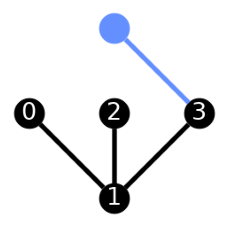
\includegraphics[width=\linewidth]{image/coupling_map_trivial_basic.png}
        \caption{One-to-one mapping}
        \label{fig:one-to-one-mapping}
    \end{subfigure}
    \hfill
    \begin{subfigure}{0.7\linewidth}
        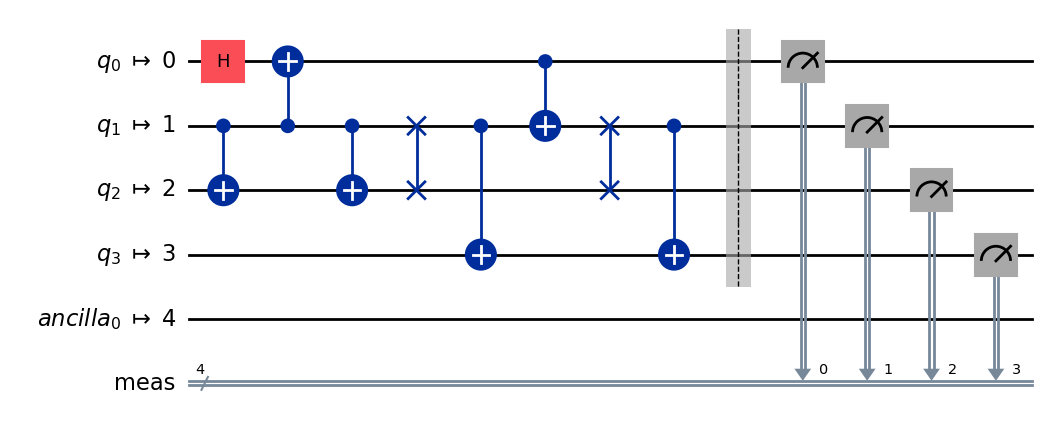
\includegraphics[width=\linewidth]{image/swap_trivial_basic.png}
        \caption{Transpiled quantum circuit with basic swap routing}
        \label{fig:swap-trivial-basic}
    \end{subfigure}
    \hfill
    \begin{subfigure}{0.25\linewidth}
        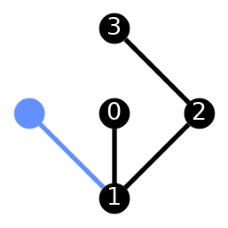
\includegraphics[width=\linewidth]{image/coupling_map_lookahead.png}
        \caption{Interaction layout mapping}
        \label{fig:interaction-mapping}
    \end{subfigure}
    \hfill
    \begin{subfigure}{0.7\linewidth}
        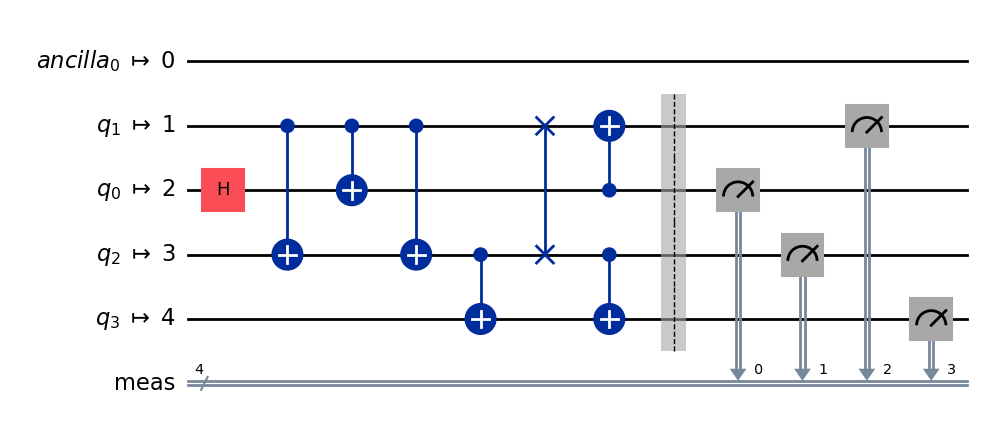
\includegraphics[width=\linewidth]{image/swap_lookahead.png}
        \caption{Transpiled quantum circuit with lookahead swap routing}
        \label{fig:swap-lookahead}
    \end{subfigure}
    \caption{Comparison between layout and routing implementation}
\end{figure}

\subsection{Transformation Pass} % done turnitin
The Pass Manager responsible for routing requires the use of a \lstinline{TransformationPass} \cite{ibmquantum_transformationpass} to modify the \acrshort{dag} structure representing the quantum circuit. This pass manager takes the device's coupling map and the circuit's \acrshort{dag} as inputs and modifies the \acrshort{dag} by inserting the necessary swap gates to ensure that the circuit adheres to the hardware coupling constraints. The output of this process is a transpiled quantum circuit that is compatible with the physical device and ready for execution.

\section{Integration}
\subsection{Staged Pass Manager} % done chat, turnitin
The final step involves integrating both Algorithm \ref{alg:interaction-layout-mapping} \mycode{Interaction Layout Mapping} and Algorithm \ref{alg:lookahead-swap-routing} \mycode{Dynamic Lookahead Swap Routing} into the Staged Pass Manager. In this pass manager, the \lstinline{init} stage unrolls gates involving more than three qubits, and \lstinline{layout} applies the most effective interaction layout mapping. The \lstinline{routing} generates the minimal number of SWAP gates required to satisfy the device's coupling constraints. The final stage, \lstinline{translation}, converts the logical gates into the available basis gate set for the selected device backend. By employing this staged pass manager, the initial quantum circuit is fully translated and optimized for execution on the target backend. \\
For instance, the initial circuit shown in Figure \ref{fig:circuit-init} has a circuit size of 11 and a circuit depth of 6. When using the \lstinline{TrivialLayout} and \lstinline{BasicSwap} methods, as depicted in Figure \ref{fig:swap-trivial-basic}, the circuit size increases to 17 and depth to 13 (Figure \ref{fig:routing-basic-swap}). In contrast, the \lstinline{InteractionLayout} and \lstinline{LookaheadSwap} methods, as shown in Figure \ref{fig:swap-lookahead}, produce a more compact circuit with a size of 14 and a depth of 9 (Figure \ref{fig:routing-lookahead}).

\begin{figure}[htb]
    \centering
    \begin{subfigure}{0.8\linewidth}
        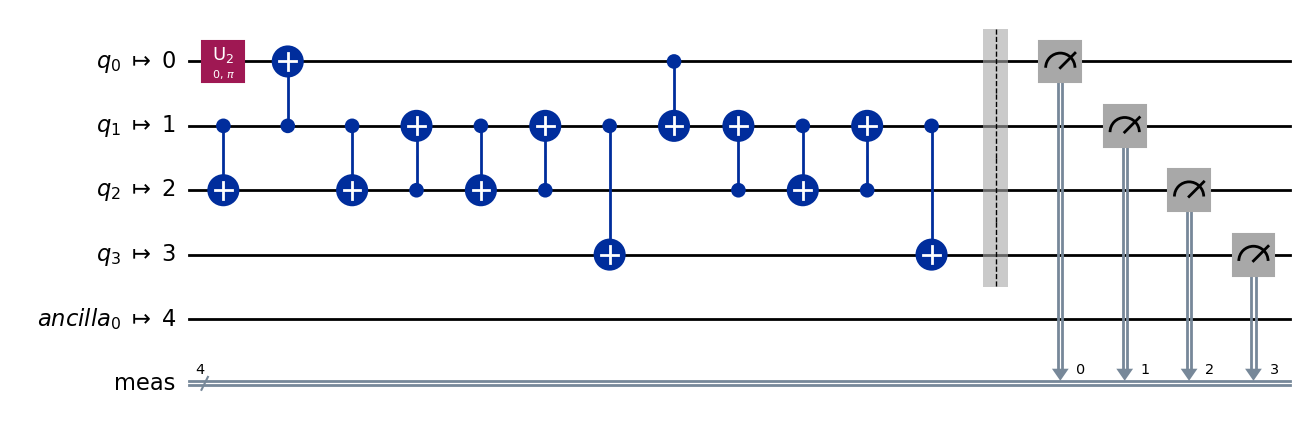
\includegraphics[width=\linewidth]{image/final_trivial_basic.png}
        \caption{Translated final layout with \lstinline{BasicSwap} routing, with additional 2 SWAPs}
        \label{fig:routing-basic-swap}
    \end{subfigure}
    \begin{subfigure}{0.8\linewidth}
        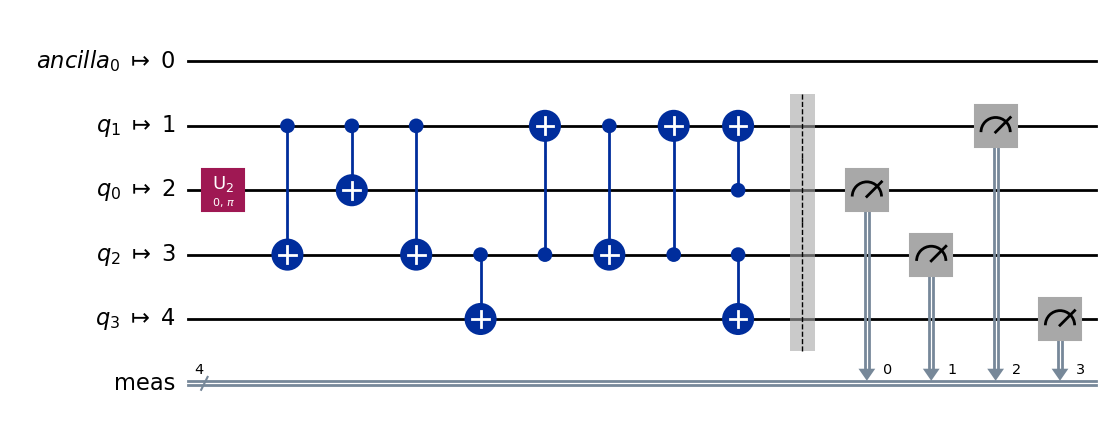
\includegraphics[width=\linewidth]{image/final_lookahead.png}
        \caption{Translated final layout with \lstinline{Lookahead} routing, with additional 1 SWAP}
        \label{fig:routing-lookahead}
    \end{subfigure}
    \caption{Comparison for swap gate routing methods}
\end{figure}

\subsection{Verification} % done chat, turnitin
The verification process involves retrieving the results of a quantum computation after a job has been executed on a quantum device or simulator. For this work, \lstinline{GenericBackend2} \cite{ibmquantum_genericbackendv2} is used, and the backend is run without noise. The result is returned as a dictionary, where the keys represent the bitstrings of the measured qubits, and the values represent the number of times each bitstring was measured. This output allows for the analysis of the probability distribution of the qubit states after the quantum circuit has been executed. \\
The \lstinline{Result} class \cite{ibmquantum_result} of the transpiled quantum circuit, run on Qiskit's preset pass manager, is then compared with the result obtained from the algorithm's swap implementation. It is observed that several of the highest occurrences are identical in both cases (Figure \ref{fig:plot-basic} and Figure \ref{fig:plot-lookahead}), indicating consistency between the two methods.
\begin{figure}[htb]
    \centering
    \begin{subfigure}{0.45\linewidth}
        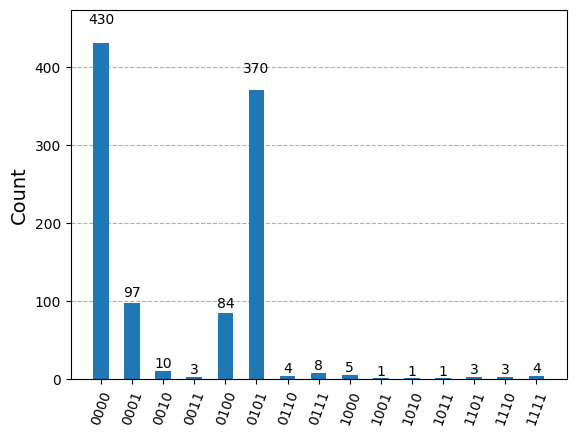
\includegraphics[width=\linewidth]{image/plot_basic.png}
        \caption{Result counts from \lstinline{BasicSwap} method}
        \label{fig:plot-basic}
    \end{subfigure}
    \begin{subfigure}{0.45\linewidth}
        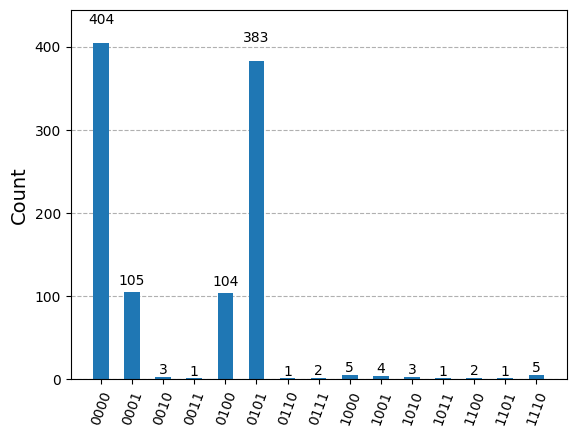
\includegraphics[width=\linewidth]{image/plot_lookahead.png}
        \caption{Result counts of \lstinline{Lookahead}}
        \label{fig:plot-lookahead}
        \end{subfigure}
    \caption{Result counts from running \lstinline{FakeLondonV2} backend. The counts vary due to being drawn from probability distributions, with the highest occurrences being compared.}
\end{figure}
%%%%%%%%%%%%%%%%%%%%%%%%%%%%%%%%%%%%%%%%%%%%%%%%%%%%%%%%%%%%%%%%%%%%%%%%%%%%%%%%
\chapter{Results and Analysis} \label{Chap4}
\section{Configurations} % done chat, turnitin
The evaluation is configured as follows:
\begin{enumerate}[nolistsep]
    \item Metrics: The evaluation focuses on two main metrics, the total number of additional swap gates $(g)$ and the resulting circuit depth $(d)$ after transpilation.
    \item Experiment Software: The algorithm is implemented in Python version 3.10.12 with IBM Qiskit framework. The code is available on Github \url{https://github.com/natashaval/qubit-mapping-distributed-qc}.
    \item Experiment Hardware: The tests were conducted on a standard personal computer equipped with an Intel i7-8700 CPU and 16 GB of RAM.
    \item Layout: The algorithms were tested using 20 qubits across the layouts detailed in Table  \ref{tab:layout-qubit-group}. The layout names follow the format: \textit{<layout name>\_<number of qubits>\_<number of groups>}. Each layout is a symmetric coupling graph, enabling bidirectional operation of two-qubit gates between any pair of connected physical qubits. Coupling graphs are illustrated in Appendix \ref{app:coupling-graph-by-group}.
        \begin{table}[htb]
\centering
\caption{Number of qubits and group for layouts}
\label{tab:layout-qubit-group}
\begin{tabular}{|c|c|c|} 
\hline
\textbf{Layout} & \textbf{Number of qubits} & \textbf{Number of groups}  \\ 
\hline
Full            & 20                        & 1                         \\ 
\hline
Full            & 10                        & 2                         \\ 
\hline
Grid            & 9                         & 2                         \\ 
\hline
Ring            & 10                        & 2                         \\ 
\hline
Full            & 7                         & 3                         \\ 
\hline
Grid            & 8                         & 3                         \\ 
\hline
Ring            & 7                         & 3                         \\ 
\hline
Full            & 5                         & 4                         \\ 
\hline
Grid            & 6                         & 4                         \\ 
\hline
Ring            & 5                         & 4                         \\ 
\hline
T Horizontal    & 5                         & 4                         \\ 
\hline
T Vertical      & 5                         & 4                         \\ 
\hline
Line            & 1                         & 20                        \\
\hline
\end{tabular}
\end{table}
    \item Benchmarks: The benchmarks  listed in Table \ref{tab:table-algorithm-size-depth} are taken from MQTBench \cite{quetschlich_mqt_2023}. The quantum circuits are composed of native gates from the Qiskit library and are represented in the QASM 2.0 language.
        \begin{table}[htb]
\centering
\caption{Circuit size and circuit depth of benchmark algorithms for 5, 10, and 15 qubits}
\label{tab:table-algorithm-size-depth}
\begin{tabular}{|l|c|c|c|c|c|c|} 
\hline
\multicolumn{1}{|c|}{\textbf{Algorithm}} & \multicolumn{2}{c|}{\textbf{n = 5}} & \multicolumn{2}{c|}{\textbf{n = 10}} & \multicolumn{2}{c|}{\textbf{n = 15}}  \\ 
\hline
\multicolumn{1}{|c|}{\textbf{}}          & gate & depth                        & gate & depth                         & gate & depth                          \\ 
\hline
ghz                                      & 7    & 7                            & 12   & 12                            & 17   & 17                             \\ 
\hline
dj                                       & 36   & 11                           & 79   & 17                            & 118  & 22                             \\ 
\hline
graphstate                               & 50   & 22                           & 100  & 26                            & 150  & 29                             \\ 
\hline
qft                                      & 71   & 38                           & 270  & 78                            & 591  & 118                            \\ 
\hline
wstate                                   & 73   & 45                           & 163  & 90                            & 253  & 135                            \\ 
\hline
qftentangled                             & 78   & 42                           & 282  & 82                            & 608  & 122                            \\ 
\hline
vqe                                      & 83   & 21                           & 168  & 26                            & 253  & 31                             \\ 
\hline
qaoa                                     & 95   & 31                           & 190  & 34                            & 285  & 34                             \\ 
\hline
realamprandom                            & 130  & 37                           & 335  & 57                            & 615  & 77                             \\ 
\hline
twolocalrandom                           & 130  & 37                           & 335  & 57                            & 615  & 77                             \\ 
\hline
su2random                                & 150  & 41                           & 375  & 61                            & 675  & 81                             \\ 
\hline
qnn                                      & 154  & 58                           & 459  & 108                           & 914  & 158                            \\ 
\hline
portfolioqaoa                            & 195  & 72                           & 615  & 132                           & 1260 & 192                            \\ 
\hline
random                                   & 223  & 97                           & 646  & 155                           & 1992 & 412                            \\ 
\hline
portfoliovqe                             & 310  & 107                          & 1145 & 217                           & 2505 & 327                            \\
\hline
\end{tabular}
\end{table}
\end{enumerate}

\section{Evaluation}
The data is processed from the table in the appendix \ref{app:benchmark-result-table-by-group}.
\subsection{Distribution of Additional Swap Gates and Circuit Depth} % done chat
The box plot in Figure \ref{fig:chart-box-plot-swap} compares the average number of additional swap gates required by three different strategies, namely \lstinline{BasicSwap}, \lstinline{SabreSwap}, and \lstinline{LookaheadSwap}, across various layout configurations. \lstinline{BasicSwap} \cite{ibmquantum_basicswap} strategy employs a brute force approach, adding one or more swap gates whenever a connectivity constraint is encountered, iterating through each layer until the circuit is compatible. The \lstinline{SabreSwap} strategy uses a heuristic search to minimize the number of swap gates and reduce circuit depth \cite{li_tackling_2019, ibmquantum_sabreswap}. Meanwhile, the \lstinline{LookaheadSwap} strategy combines elements from both algorithms (Algorithm \ref{alg:interaction-layout-mapping} and \ref{alg:lookahead-swap-routing}) that has been described in the previous section. A lower number of swap gates or fewer circuit depth indicates better strategy performance. \\
The \lstinline{BasicSwap} consistently exhibits the highest number of swap gates across all layouts, with particularly high values exceeding 5000 additional swap gates in layouts such as \textit{ring\_10\_2}, \textit{t\_horizontal\_5\_4}, \textit{t\_vertical\_5\_4}, and performing worst in the \textit{line\_1\_20} layout. The large spread and height of the boxes indicate both poor and inconsistent performance. In contrast, \lstinline{SabreSwap} performs significantly better with the range of around 1000 additional swap gates for all layouts. \lstinline{LookaheadSwap} performs almost as well as \lstinline{SabreSwap}, with the best results seen in the \textit{full\_7\_3} layout. However, in some cases like \textit{full\_5\_4} and \textit{ring\_5\_4}, the \lstinline{LookaheadSwap} strategy has exceptionally low values that are likely outliers due to timeouts, which may skew the perception of its effectiveness in these instances. \\
Overall, the layouts that show better performance, as indicated by lower swap gate counts, are \textit{grid\_8\_3}, \textit{grid\_6\_4}, \textit{full\_10\_2} and \textit{full\_7\_3}. These results suggest that \textit{grid} and \textit{full} layouts are generally more efficient than other configurations. It is also important to note that \textit{full\_20\_1} and \textit{line\_1\_20} serve as baselines; \textit{full\_20\_1} represents a maximally connected coupling map and is expected to deliver the best performance, while \textit{line\_1\_20}, being the least connected, is likely to show the poorest performance. \\
\begin{figure}[htb]
    \centering
    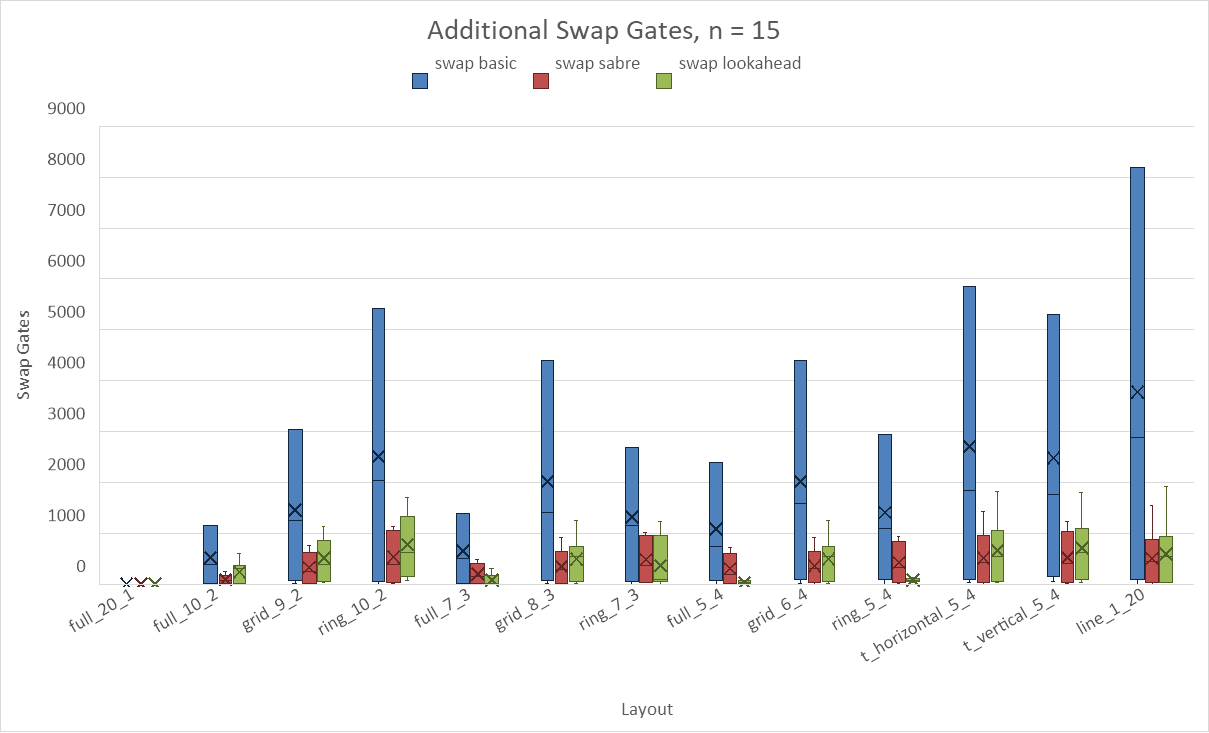
\includegraphics[width=0.9\linewidth]{image/chart_box_plot_swap.png}
    \caption{Box plot additional swap gates for a circuit size of 15}
    \label{fig:chart-box-plot-swap}
\end{figure}

Similarly, the analysis of quantum circuit depths across various layouts, as shown in Figure \ref{fig:chart-box-plot-depth}, reveals significant differences in the effectiveness of the three optimization methods. The depths associated with \lstinline{BasicSwap} consistently result in the highest circuit depths often exceeding 1000, and in some cases approach 2000 or more in layouts like \textit{line\_1\_20}, \textit{t\_horizontal\_5\_4}, and \textit{ring\_10\_2}. In contrast, \lstinline{SabreSwap} and \lstinline{LookaheadSwap} both achieve significantly shallower circuit depths, generally clustering below 500. However, some layouts, such as \textit{full\_5\_4} and \textit{ring\_5\_4} show occasional outliers. \\
Overall, the \lstinline{SabreSwap} and \lstinline{LookaheadSwap} strategies perform comparably well, with the latter slightly outperforming \lstinline{SabreSwap} in certain configurations. The most efficient layouts, characterized by lower circuit depths, include \textit{full\_7\_3} and \textit{grid\_6\_4}, where both \lstinline{SabreSwap} and \lstinline{LookaheadSwap} consistently maintain minimal circuit depth. This suggests that for minimizing circuit depth, \lstinline{LookaheadSwap} is generally the most effective strategy, closely followed by \lstinline{SabreSwap}.
\begin{figure}[htb]
    \centering
    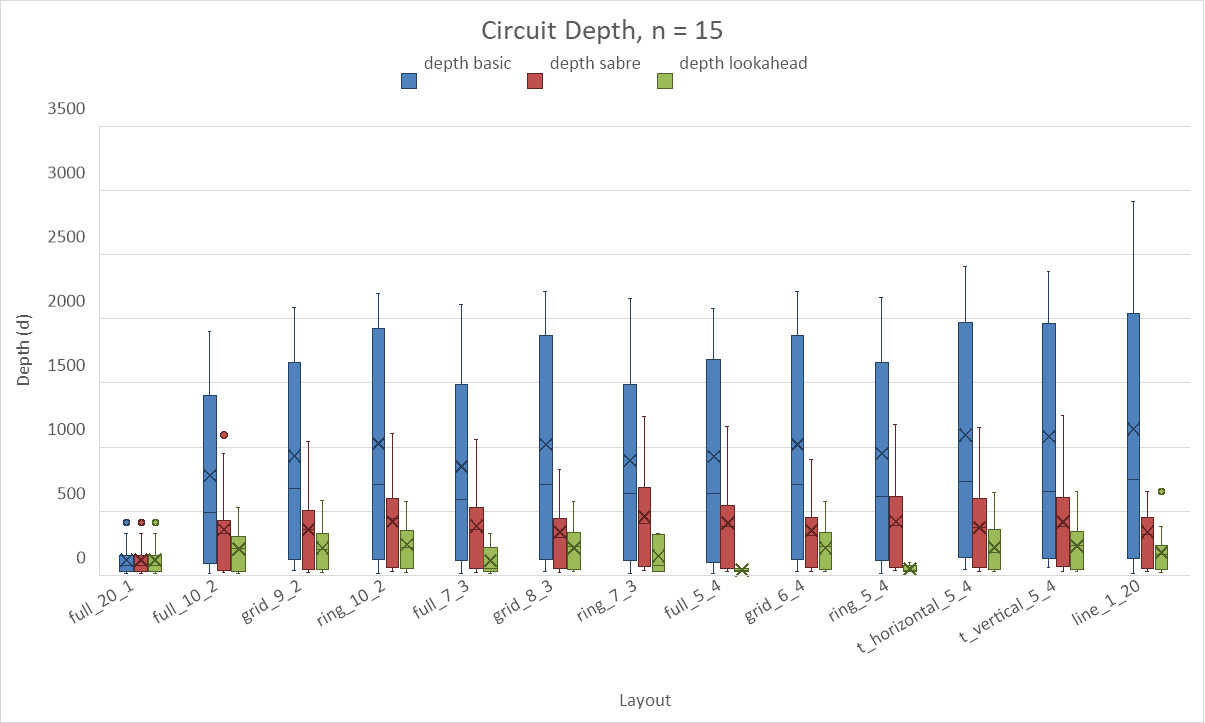
\includegraphics[width=\linewidth]{image/chart_box_plot_depth.png}
    \caption{Box plot circuit depth for a circuit size of 15}
    \label{fig:chart-box-plot-depth}
\end{figure}

The box plots present the additional swap gates \ref{fig:chart-box-plot-group} and circuit depth \ref{fig:chart-box-plot-group-depth} categorized by group for a circuit size of 15.  Group 1 and Group 20 serve as baselines, with Group 1 representing a fully connected graph and Group 20 a line coupling graph. Among other groups, Group 2 stands out as the best performer. In Group 2, the \lstinline{LookaheadSwap} strategy performs particularly well, showing very low swap gate counts and moderate circuit depths, reflecting consistent and efficient performance. Group 3, while similar to Group 2, displays slightly more variability in circuit depths and a minor increase in swap gate counts, particularly with the \lstinline{BasicSwap} strategy, though the \lstinline{LookaheadSwap} approach still outperforms the others. Group 4, on the other hand, shows the most variability, especially with the \lstinline{BasicSwap} strategy, which has a much higher median and a widespread, suggesting inconsistent performance. Although the \lstinline{LookaheadSwap} strategy in Group 4 still achieves the lowest swap gate counts and circuit depths, its performance is less consistent compared to Groups 2 and 3. Therefore, Group 2 emerges as the top performer in minimizing swap gates and lowering circuit depths with the \lstinline{LookaheadSwap} strategy, followed by Group 3, while Group 4 shows the least favourable results. \\
\begin{figure}[htb]
    \centering
    \begin{subfigure}{0.48\linewidth}
        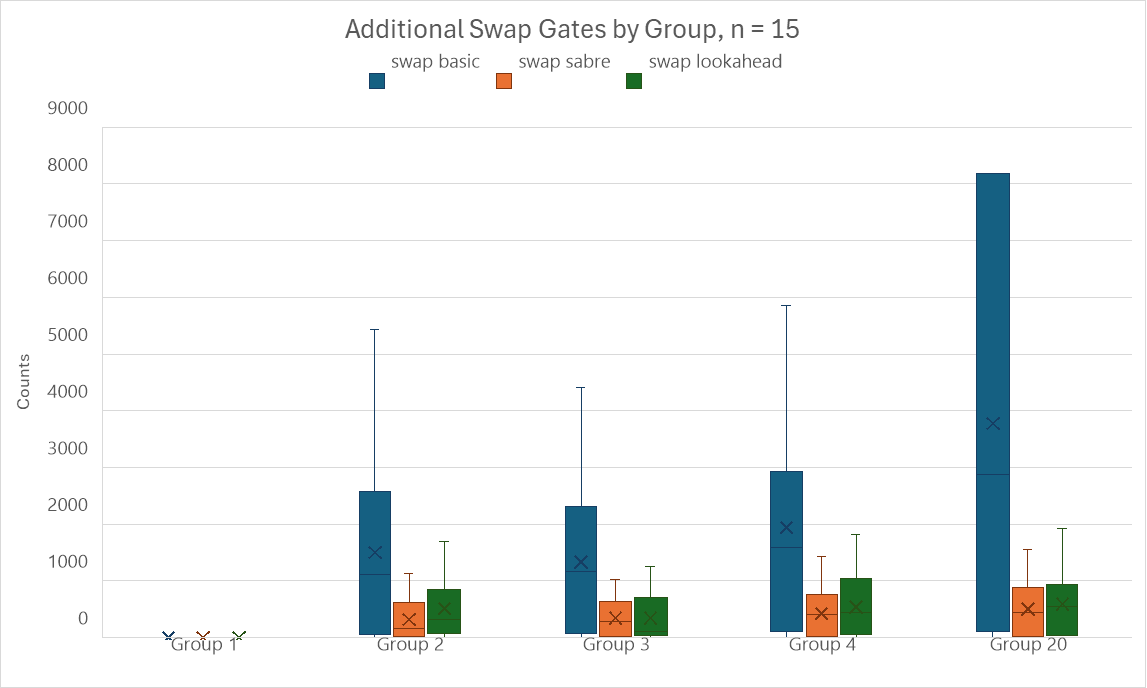
\includegraphics[width=\linewidth]{image/chart_box_plot_group.png}
        \caption{Box Plot Additional Swap Gates by Group}
        \label{fig:chart-box-plot-group}
    \end{subfigure}
    \begin{subfigure}{0.48\linewidth}
        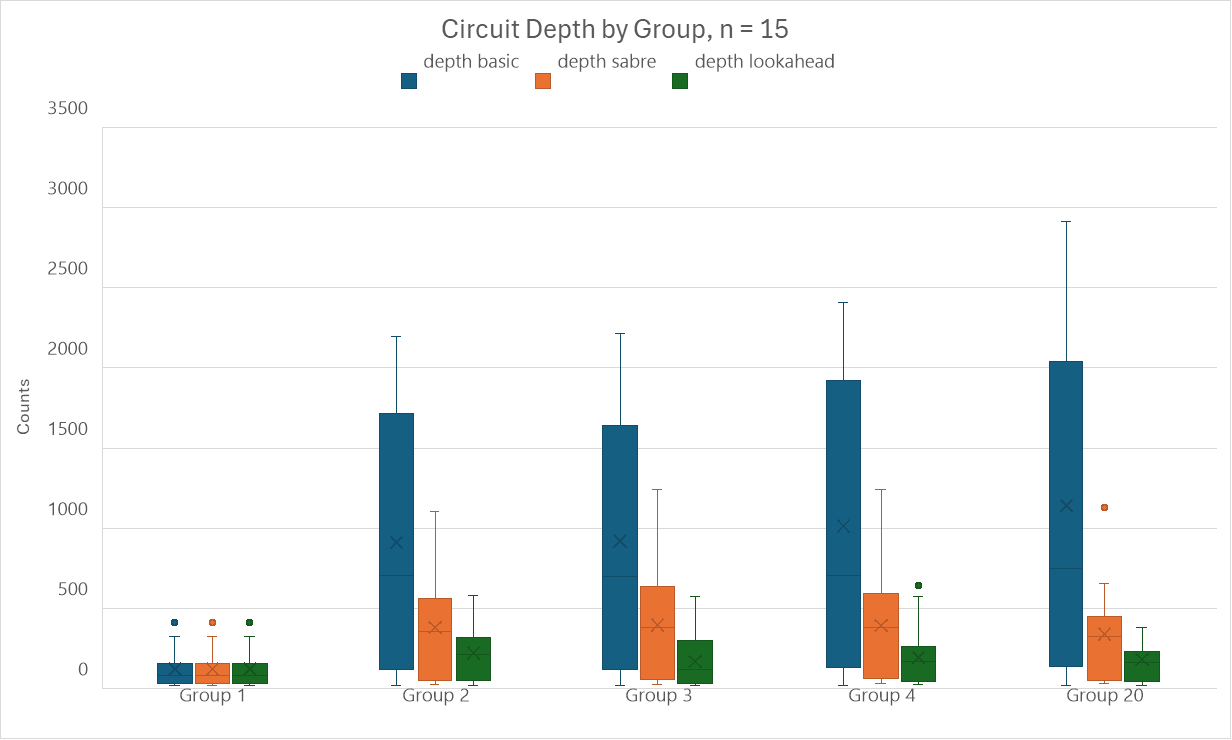
\includegraphics[width=\linewidth]{image/chart_box_plot_group_depth.png}
        \caption{Box Plot Circuit Depth by Group}
        \label{fig:chart-box-plot-group-depth}
    \end{subfigure}
    \caption{Swap strategies categorized in group for a circuit size of 15}
    \label{fig:chart-box-plot-group-all}
\end{figure}

\subsection{The Total Number of Algorithms Successfully Run for Each Layout}
The previous section mentioned that the algorithms for the \textit{full\_5\_4} and \textit{ring\_5\_4} layouts show outliers, indicating that they do not execute all the algorithms. Therefore, the chart in Figure \ref{fig:chart-success-algorithm-run} specifies the total number of successful algorithms run across different layouts, focusing on circuit sizes ranging from 5, 10, and 15 qubits, with a total of 15 algorithms per round. Most layouts perform consistently well, achieving the maximum count of 15 successful runs per benchmark. \\
One thing to notice is that \textit{full\_7\_3} and \textit{full\_5\_4}  layouts fail to complete the benchmarks for the largest circuit size of 15 qubits, with \textit{full\_7\_3} achieving only 9 successful runs and \textit{full\_5\_4} barely completing 3 runs. Additionally, \textit{ring\_7\_3} and \textit{ring\_5\_4} layouts also encounter difficulties, particularly as the circuit size increases beyond 10 qubits. \textit{Ring\_7\_3} can only achieve 10 and 8 successful runs for circuit sizes 10 and 15, while \textit{ring\_5\_4} struggles even at the 5-qubit benchmark, with its performance worsening as the circuit size increases. The failed algorithms and layouts are listed in Appendix \ref{app:failed-algorithm-layout}. \\
These variations suggest that certain layouts are more robust across different run sizes, while others, particularly \textit{ring\_7\_3} and \textit{ring\_5\_4} face challenges with medium run sizes, indicating possible inefficiencies or challenges in these configurations. In general, the layouts in groups 1 and 2 are more consistent across different run sizes, while those in groups 3 and 4 tend to show more variability.
\begin{figure}[htb]
    \centering
    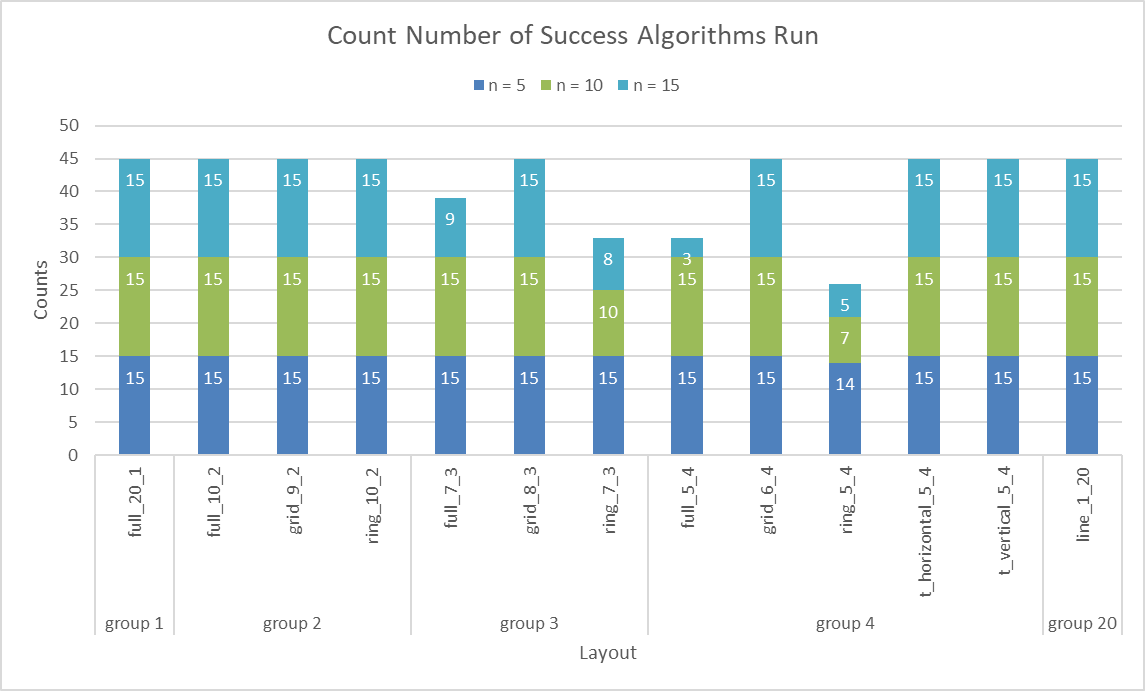
\includegraphics[width=0.8\linewidth]{image/chart_success_algorithm_run.png}
    \caption{Total count of successful algorithm runs across various layouts, $n = 15$}
    \label{fig:chart-success-algorithm-run}
\end{figure}

In addition, the chart in Figure \ref{fig:chart-success-layout-run} highlights the total count of successful layout executions across different algorithms. Most algorithms like "dj", "graphstate" and "qaoa" maintain consistent performance across all benchmark sizes with 100\% success rate. However, some algorithms, like "qft", "qftentangled", "realamprandom", and "twolocalrandom", show slightly reduced success rates, particularly for $n = 10$, where the count drops to 12. The algorithms "qnn" and "random" display even more pronounced variations, with success rates for $n = 10$ and $n = 15$ decreasing to 11 and 9, respectively. \\
While most algorithms perform reliably across all benchmarks, a few show inconsistencies, especially with $n = 10$ and $n = 15$, suggesting that certain algorithms may struggle with larger problem sizes.
\begin{figure}[htb]
    \centering
    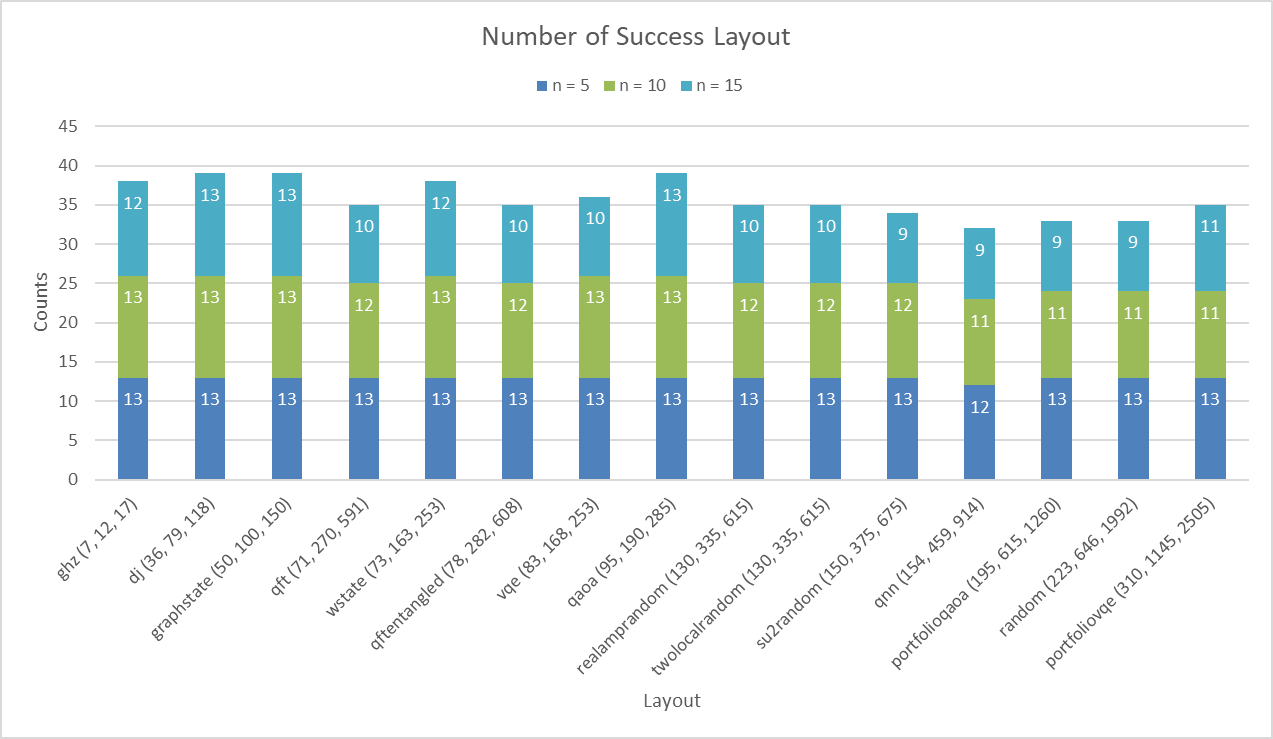
\includegraphics[width=0.8\linewidth]{image/chart_success_layout_run.png}
    \caption{Total count of successful layouts across different algorithms}
    \label{fig:chart-success-layout-run}
\end{figure}
\FloatBarrier

\subsection{Layouts for Algorithms}
In this section, a selection of representative algorithms - GHZ, Deutsch-Jozsa, Graph State, VQE, and Portfolio QAOA - are analyzed and compared across various layouts. The baseline values for the total circuit gates and circuit depth are provided in parentheses, and the results discussed are based on using 15 qubits. This comparison highlights how different layouts perform when subjected to different swap routing methods.

\subsection{GHZ} % done chat
The GHZ charts compare the number of additional swap gates needed for different layouts (Figure \ref{fig:chart-ghz}) and the resulting circuit depth (Figure \ref{fig:chart-ghz-depth}) when running with 17 qubits. It shows that the \lstinline{BasicSwap} strategy generally performs best, requiring the fewest swaps, particularly in all full, ring, and line layouts, where it results in 0 additional swap gates. In this context, \lstinline{SabreSwap} tend to perform worse than \lstinline{BasicSwap}, while the \lstinline{LookaheadSwap} strategy performs significantly worse than the others, with a notable spike in the \textit{ring\_10\_2} layout. Regarding circuit depth, the results for \lstinline{LookaheadSwap} are nearly comparable to those of \lstinline{SabreSwap}, with both strategies yielding a circuit depth of approximately 30.
\begin{figure}[htb]
    \centering
    \begin{subfigure}{0.48\linewidth}
        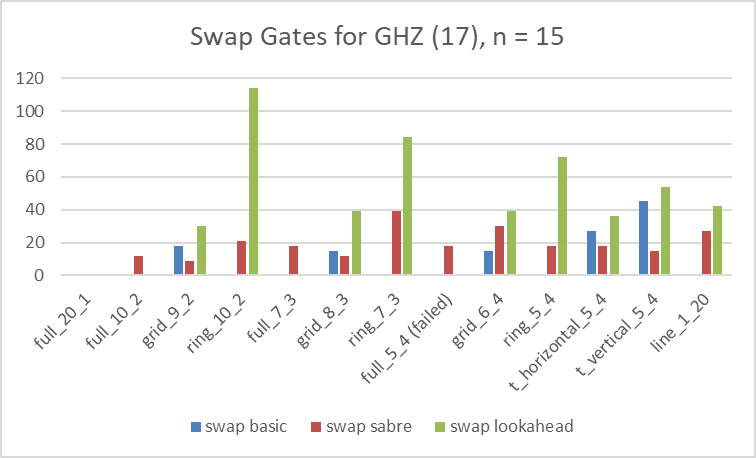
\includegraphics[width=\linewidth]{image/chart_ghz.png}
        \caption{Additional swap gates for GHZ}
        \label{fig:chart-ghz}
    \end{subfigure}
    \begin{subfigure}{0.48\linewidth}
        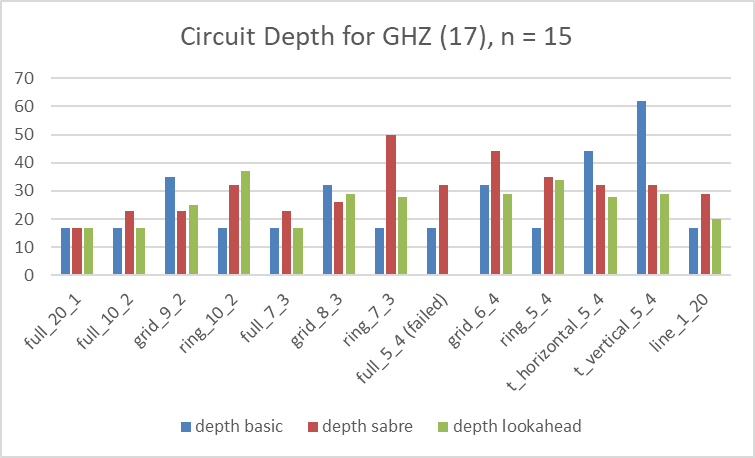
\includegraphics[width=\linewidth]{image/chart_ghz_depth.png}
        \caption{Circuit depth for GHZ}
        \label{fig:chart-ghz-depth}
    \end{subfigure}
\end{figure}

\subsection{Deutsch-Jozsa} % done chat
The charts for running the Deutsch-Jozsa algorithm with 118 gates (Figure \ref{fig:chart-dj}) and a circuit depth of 22 (Figure \ref{fig:chart-dj-depth}) show that the \lstinline{SabreSwap} and \lstinline{LookaheadSwap} strategies consistently outperform the \lstinline{BasicSwap} strategy in minimizing swap gates. The \textit{line\_20\_1} layout performs poorly, with the \lstinline{BasicSwap} method leading to an extremely high number of additional swap gates, exceeding 500. Although the additional swap gates for \lstinline{SabreSwap} and \lstinline{LookaheadSwap} are similar across all layouts, remaining below 50, the circuit depth with \lstinline{LookaheadSwap} is significantly lower, staying under 40 for all layouts, compared to \lstinline{SabreSwap}, which is around 60.
\begin{figure}[htb]
    \centering
    \begin{subfigure}{0.48\linewidth}
        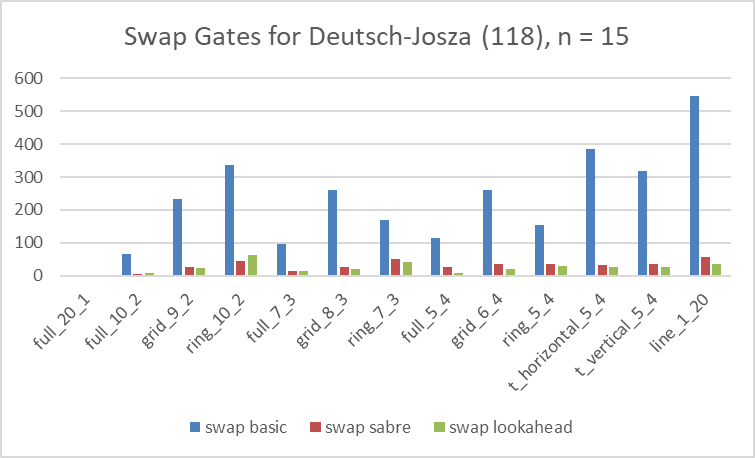
\includegraphics[width=\linewidth]{image/chart_dj.png}
        \caption{Additional swap gates for Deutsch-Jozsa}
        \label{fig:chart-dj}
    \end{subfigure}
    \begin{subfigure}{0.48\linewidth}
        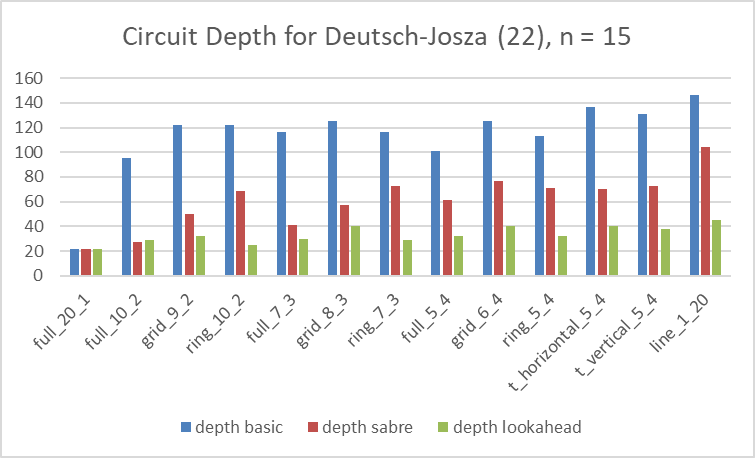
\includegraphics[width=\linewidth]{image/chart_dj_depth.png}
        \caption{Circuit depth for Deutsch-Jozsa}
        \label{fig:chart-dj-depth}
    \end{subfigure}
\end{figure}

\subsection{Graph State} % done chat
The Graph State charts compare additional swap gates with an initial count of 150 gates (Figure \ref{fig:chart-graphstate}) and a circuit depth of 30 (Figure \ref{fig:chart-graphstate-depth}) across different layouts. In this algorithm, the performance of \lstinline{LookaheadSwap} is similar to \lstinline{BasicSwap}, with the poorest performance observed in the \textit{t\_vertical\_5\_4} layout, which requires 120 additional swap gates. The \lstinline{SabreSwap} strategy, on the other hand, results in significantly fewer swap gates, with counts around 20. Despite the difference in additional swap gates between \lstinline{SabreSwap} and \lstinline{LookaheadSwap} being as much as 200\%, the resulting circuit depth is almost comparable, ranging from 30 to 40 across all layouts.
\begin{figure}[htb]
    \centering
    \begin{subfigure}{0.48\linewidth}
        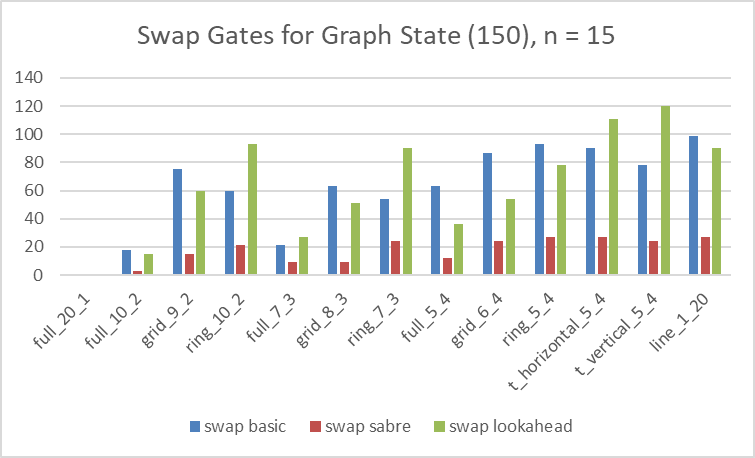
\includegraphics[width=\linewidth]{image/chart_graphstate.png}
        \caption{Additional swap gates for Graph State}
        \label{fig:chart-graphstate}
    \end{subfigure}
    \begin{subfigure}{0.48\linewidth}
        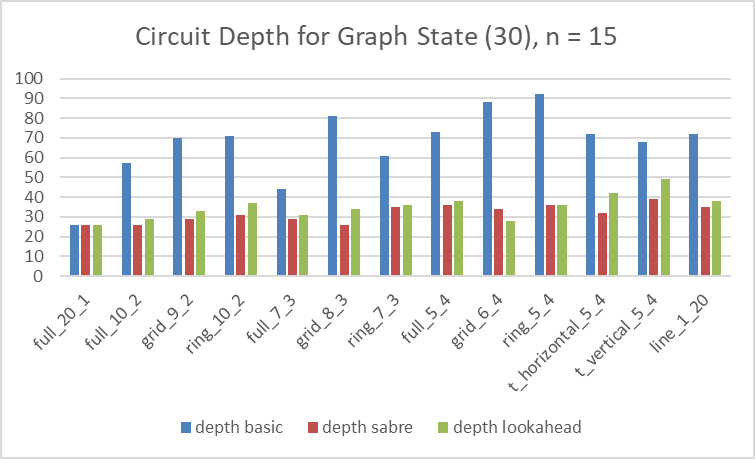
\includegraphics[width=\linewidth]{image/chart_graphstate_depth.png}
        \caption{Circuit depth for Graph State}
        \label{fig:chart-graphstate-depth}
    \end{subfigure}
\end{figure}

\subsection{VQE}
The chart illustrates that for the VQE algorithm with 253 gates (Figure \ref{fig:chart-vqe}), the \lstinline{SabreSwap} strategy generally performs best across most layouts, particularly in \textit{grid\_8\_3}, \textit{grid\_6\_4} and \textit{t\_horizontal\_5\_4}, where it minimizes the number of additional swap gates. In contrast, the \lstinline{LookaheadSwap} strategy tends to require significantly more swaps, especially in layouts like \textit{ring\_10\_2} and \textit{t\_vertical\_5\_4}. The \lstinline{BasicSwap} strategy shows similar behaviour to \lstinline{LookaheadSwap}, with the exception of the \textit{t\_vertical\_5\_4} layout, where it exceeds 140 additional swap gates. When examining circuit depth (Figure \ref{fig:chart-vqe-depth}), \lstinline{BasicSwap} does not show much difference from the baseline, remaining at 31. Meanwhile, the circuit depth performance of \lstinline{LookaheadSwap} is comparable to that of \lstinline{SabreSwap}, with layouts like \textit{full\_7\_3} and \textit{t\_vertical\_5\_4} delivering significantly better results, with a reduction of nearly 40\%.
\begin{figure}[htb]
    \centering
    \begin{subfigure}{0.48\linewidth}
        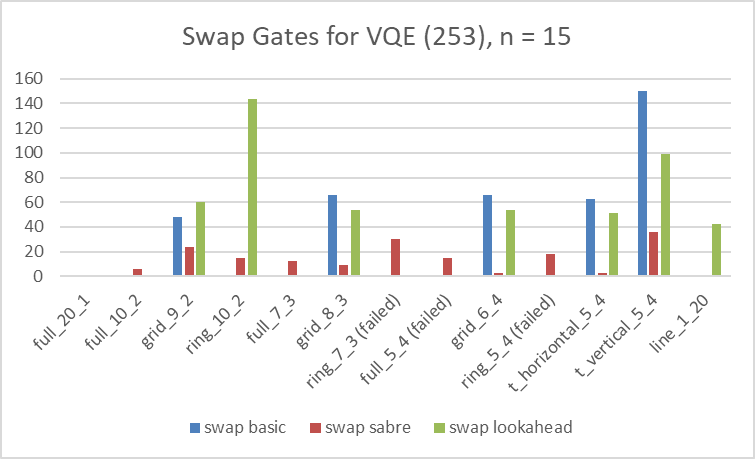
\includegraphics[width=\linewidth]{image/chart_vqe.png}
        \caption{Additional swap gates for VQE}
        \label{fig:chart-vqe}
    \end{subfigure}
    \begin{subfigure}{0.48\linewidth}
        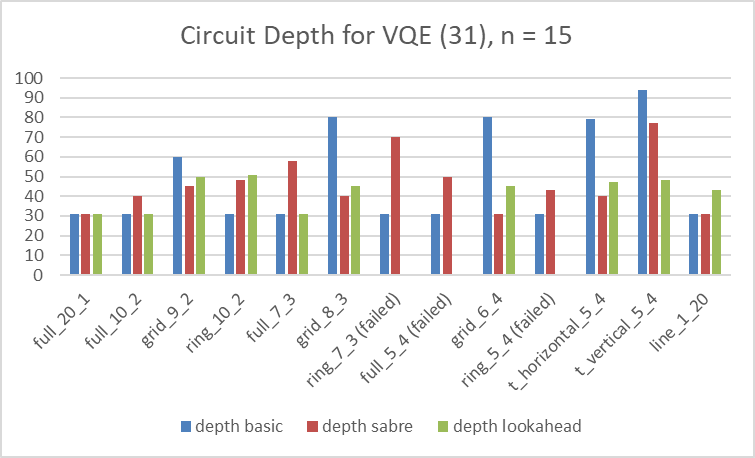
\includegraphics[width=\linewidth]{image/chart_vqe_depth.png}
        \caption{Circuit depth for VQE}
        \label{fig:chart-vqe-depth}
    \end{subfigure}
\end{figure}

\subsection{Portfolio QAOA}
These final charts serve as representatives for various other algorithms listed in Table \ref{tab:table-algorithm-size-depth}, ranging from "qft" to "portfoliovqe". The charts compare the performance of swap strategies for the Portfolio QAOA algorithm with 1260 gates (Figure \ref{fig:chart-portfolioqaoa}) and a circuit depth of 192 (Figure \ref{fig:chart-portfolioqaoa-depth}). The \lstinline{BasicSwap} strategy performs poorly, especially in layouts like \textit{ring\_10\_2}, \textit{t\_horizontal\_5\_4}, and \textit{line\_1\_20} with swap counts exceeding 5000 in some cases. On the other hand, both \lstinline{SabreSwap} and \lstinline{LookaheadSwap} significantly reduce the number of swap gates across most layouts to just below 2000, with \lstinline{SabreSwap} generally requiring fewer swaps than \lstinline{LookaheadSwap}. The second chart showing circuit depth follows a similar pattern: \lstinline{BasicSwap} results in much deeper circuits, often exceeding 2000 in depth, particularly in the same problematic layouts. \lstinline{SabreSwap} and \lstinline{LookaheadSwap} again perform better, with \lstinline{SabreSwap} consistently achieving lower circuit depths around 700, closely followed by \lstinline{LookaheadSwap} just below 500.
\begin{figure}[htb]
    \centering
    \begin{subfigure}{0.48\linewidth}
        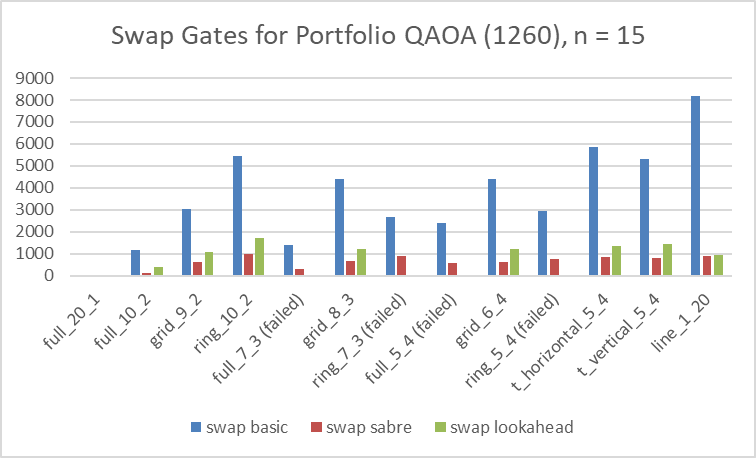
\includegraphics[width=\linewidth]{image/chart_portfolioqaoa.png}
        \caption{Additional swap gates for Portfolio QAOA}
        \label{fig:chart-portfolioqaoa}
    \end{subfigure}
    \begin{subfigure}{0.48\linewidth}
        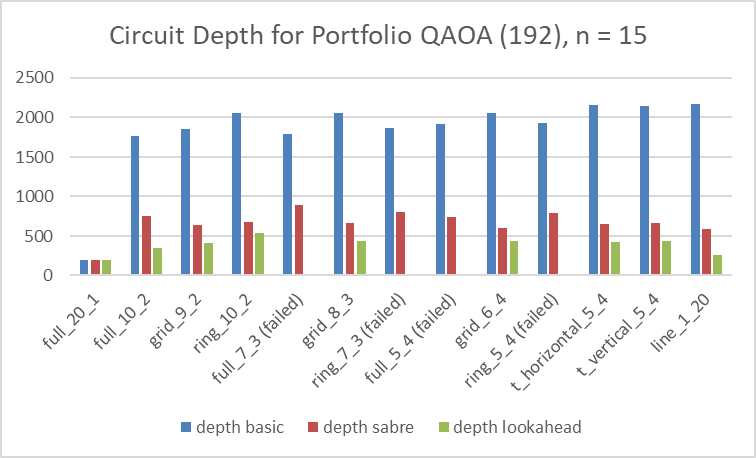
\includegraphics[width=\linewidth]{image/chart_portfolioqaoa_depth.png}
        \caption{Circuit depth for Portfolio QAOA}
        \label{fig:chart-portfolioqaoa-depth}
    \end{subfigure}
\end{figure}
%%%%%%%%%%%%%%%%%%%%%%%%%%%%%%%%%%%%%%%%%%%%%%%%%%%%%%%%%%%%%%%%%%%%%%%%%%%%%%%%
\chapter{Discussion} \label{Chap5} % NEED ALGORITHM DiSCUSSION WHICH SUITABLE FOR LAYOUT, CHECK FOR CHAT, and TURNITIN
\section{Time Complexity}
\subsection{Interaction Mapping Layout} % done chat
The Algorithm \ref{alg:interaction-layout-mapping} \mycode{InteractionLayoutMapping}, particularly the \mycode{calculate\_final\_maps} method, can be computationally intensive, especially in the worst-case scenario. During its execution, several key operations contribute to its complexity. Initially, the algorithm performs pre-processing steps, such as generating the \acrfull{qpi} matrix and calculating logical priorities and physical connectivity. These steps run in polynomial time relative to the number of physical qubits and two-qubit operations in the \acrshort{dag}. However, the main challenge arises in the core loop of the \mycode{calculate\_final\_maps} function, where the algorithm iteratively assigns logical qubits to physical qubits. \\
During this process, the algorithm checks and updates possible mappings in a \mycode{while logical\_priority} loop, which continue until all logical qubits are assigned. Each iteration may create several new mappings, causing the number of possibilities to increase exponentially, as the algorithm must consider at a rate of $O(2^k \times |P|)$, where $k$ is the recursion depth and $|P|$ is the number of physical qubits. As a result, the overall time complexity in the worst case is \textbf{exponential}, potentially reaching $O(2^k \times |P| \times n)$, where $n$ is the number of logical qubits. This exponential growth is due to the combinatorial nature of the problem, where multiple candidate mappings are explored and expanded. In practical implementations, this could result in significant computational overhead as the number of qubits increases.

\subsection{Lookahead Swap Routing} % done chat
The Algorithm \ref{alg:lookahead-swap-routing} \mycode{DynamicLookaheadSwap} is a heuristic method designed to map logical qubits to physical qubits in quantum circuits, especially on hardware with limited connectivity. The goal of the algorithm is to reduce the number of additional swap gates required when implementing the circuit on the target hardware, consequently, reducing the circuit depth as well. \\
The algorithm begins with an initialization phase, where it preprocesses the quantum circuit and sets up necessary data structures. This phase runs in linear time proportional to the number of gates. The algorithm then categorizes and analyzes dependencies between gates, focusing on two-qubit operations. This step is also a linear time complexity of $O(G)$, where $G$ is the total number of two-qubit gates in the \acrshort{dag}. \\
In the main loop, the algorithm iterates over each layer of the circuit and checks whether the current qubit layout allows direct execution of two-qubit gates or if a swap operation is necessary. This \mycode{check\_gate\_connectivity} has a time complexity of $O(G \times n^2)$, where $n$ is the number of qubits. The algorithm then \mycode{generate\_possible\_swaps} operations by considering the neighbours of the involved qubits in the coupling map, with a complexity of $O(G \times n^2 \times D)$, where $D$ is the degree of connectivity in the coupling map. \\
For each potential swap, the algorithm evaluates its effect on the circuit using the \mycode{sum\_effect} method. This method assesses how the swap improves qubit placement for future gates by exchanging physical qubits and reducing the distance between qubits. This swap evaluation process can be computationally intensive, with a worst-case time complexity of $O(S \times G)$, where $S$ is the number of candidate swaps. If a beneficial swap is identified, it is applied to the layout at $O(1)$, which further modifies the circuit structure. \\
Overall, the worst-case time complexity of the \mycode{DynamicLookaheadSwap} algorithm is approximately $O(G \times n^2 \times D + S \times G)$, reflecting the number of two-qubit gates, qubits, and the connectivity of the coupling map. Despite the potential for high computational costs, the algorithm's use of heuristics and the pruning of less beneficial swaps helps manage its complexity, making it a practical approach for optimizing quantum circuits on devices with limited qubit connectivity.

\section{Coupling Graph Options} % done chat
\subsection{Choosing Layout}
The algorithm tested involves around 20 qubits, which aligns with previous studies \cite{li_tackling_2019, zhu_dynamic_2020} that used 5 to 20 qubits in quantum programs sourced from IBM Qiskit \cite{siraichi_qubit_2018, zulehner_efficient_2018} and RevLib \cite{wille_revlib_2008}. The chosen layout configurations - \textit{full}, \textit{grid}, \textit{ring}, \textit{t\_horizontal}, and \textit{t\_vertical} - were selected to determine which layout offers the best performance based on node connectivity. The \textit{t\_horizontal} and \textit{t\_vertical} layouts, derived from a 5-qubit T-shaped IBM backend, were specifically tested to assess how the chain's length at either end impacts qubit mapping performance. An illustration of how logical qubits are placed on physical qubits is provided in Appendix \ref{app:virtual-on-physical-illustration}. \\
When analyzing the distribution of additional swap gates, the \textit{full} layout consistently outperforms the \textit{grid} and \textit{ring} layouts. Full connectivity allows any qubit to interact directly with any other qubit, eliminating the need for intermediate swaps and ensuring the shortest path between qubits is always direct \cite{hayes_graph_2000}. The \textit{grid} layout ranks second, as it has several nodes with three neighbours, compared to the \textit{ring} layout, where each node has only two neighbours. The \textit{grid} layout requires additional operations to manage qubit connectivity, and the \textit{ring} linear layout structure further limits efficient algorithm implementation, leading to higher resource use and less efficient computation \cite{peham_optimal_2023}. The \textit{t\_horizontal\_5\_4} and \textit{t\_vertical\_5\_4} layouts show no significant difference in additional swap gates and are similar to the \textit{line\_20\_1} layout, indicating they share a linear arrangement. In summary, the number of neighbouring qubits significantly impacts the reduction of additional swap gates needed. \\
Surprisingly, the \textit{grid} layout proved to be the most stable in terms of circuit depth, successfully running all algorithms compared to the \textit{full} and \textit{ring} layouts. The \textit{t\_horizontal} and \textit{t\_vertical} layouts also performed well, running all 15 algorithms. This stability likely stems from the presence of qubits with three neighbours in these layouts, which enhances their ability to handle circuit depth effectively. Although \textit{t\_horizontal\_5\_4} and \textit{t\_vertical\_5\_4} performed similarly to \textit{line\_20\_1} in terms of additional swap gates, they exhibited slightly higher variance in circuit depth. The \mycode{DynamicLookaheadSwap} algorithm works well with these three layouts because it prioritizes executing as many active gates as possible from the dependency list while performing SWAP operations simultaneously \cite{zhang_depth_2020}. In contrast, the \textit{ring} layout is limited by its linear qubit configuration, and the \textit{full} layout struggles with large traversal nodes when evaluating swap candidates. This suggests that an optimal number of neighbouring qubits - neither too many nor too few - is necessary to maintain a balanced circuit depth when using \mycode{InteractionLayoutMapping} algorithm. \\
\subsection{Choosing Number of Groups}
According to the results shown in Figure \ref{fig:chart-box-plot-group-all}, Group 2 outperformed the other groups with low variability. This success is attributed to dividing tasks into fewer groups, which reduces the number of communication channels required between groups. With only two groups, communication overhead is minimized, as there is only one direct communication link, simplifying data exchange and reducing potential bottlenecks from waiting on other groups \cite{cuomo_optimized_2023}. In contrast, increasing the number of groups complicates coordination, requiring more complex synchronization and qubit allocation across groups \cite{cicconetti_resource_2022}. This added complexity can introduce overhead in the initial qubit mapping, as seen in the failed interaction mapping for the \textit{full\_5\_4} layout. Fewer groups result in simpler coordination, fewer dependencies to manage, and less overall system complexity. \\
In the context of networked quantum computers, it is still crucial to maintain high connectivity within the individual quantum computers inside each group. Even as tasks are divided to reduce inter-group communication overhead, the internal connectivity of each quantum computer must remain robust to ensure efficient qubit interactions. High connectivity within a quantum computer allows for more flexible and efficient execution of quantum operations, minimizing the need for additional swap gates and reducing circuit depth. This balance between minimizing communication overhead across groups and maintaining strong internal connectivity is key to optimizing the overall performance of quantum networks.

% NEED ALGORITHM DISCUSSION !!!!! compare and contrast?

\section{Limitation and Errors} % done chat
Appendix \ref{app:failed-algorithm-layout} details the layouts where timeouts occurred during quantum circuit transpilation. The \mycode{InteractionLayoutMapping} algorithm generally succeeds in mapping logical to physical qubits, except for the \textit{full\_5\_4} layout, where it failed due to a timeout during qubit placement. This issue arises because the algorithm, when traversing possible neighbours, encounters an excessively large tree. To address this, the algorithm includes an exit function that checks if the coupling map is fully connected by calculating the number of neighbours for each physical qubit. If more than 80\% of physical qubits have the maximum number of neighbours, the algorithm exits early and returns a one-to-one mapping. For example, in the best case, the \textit{full\_10\_2} layout has 9 neighbours for 18 qubits and 10 neighbours for 2 qubits that connecting groups, allowing the algorithm to detect the full connectivity and return the one-to-one mapping quickly. However, the \textit{full\_5\_4} layout, with 4 neighbours for 14 qubits and 5 neighbours for 6 qubits, fails to meet the 80\% threshold, causing the algorithm to continue exploring all possibilities until it runs out of memory. A suggested solution to overcome this problem is to analyze the local graph characteristics and check if the graph is $k$-connected \cite{cornejo_connectivity_2010}. \\
Similarly, the \mycode{DynamicLookaheadSwap} algorithm generally works well but begins to fail for certain algorithms at a circuit size of 10 in the \textit{ring\_7\_3} and \textit{ring\_5\_4} layouts, and at a circuit size of 15 in the \textit{full\_7\_3} layout, as well as the previous two layouts. The swap timeout error likely occurs due to the greedy nature of the qubit placement, which assigns logical qubits to the physical qubits with the highest connectivity. In ring layouts, the algorithm starts mapping from the center and branches out. If there are multiple active gates, the algorithm may direct one gate to a branch end but still fail to find adjacent physical qubits to operate the gate, leading to an infinite loop between two nodes at the end until timeout, as illustrated in Figure \ref{fig:swap-stuck}. One strategy to address this issue is to keep an empty list to track assigned physical qubits, but this can cause problems when multiple gates are active. If one gate completes, the next might get stuck because the necessary qubits to go back are already assigned. A potential solution could involve allowing the algorithm to backtrack to certain points in the layout and explore alternative paths \cite{parizek_fast_2019}.
\begin{figure}
    \centering
    \includegraphics[width=0.5\linewidth]{image/swap_stuck.png}
    \caption{The swap operation is stuck because the highest Lookahead value is at $Q_7$ and $Q_3$.}
    \label{fig:swap-stuck}
\end{figure}

\section{Direction of Future Work} % done chat
This section outlines potential future enhancements to optimize the current algorithm:
\begin{enumerate}[nolistsep]
    \item \textbf{Incorporating Noise}: The current work assumes quantum devices without noise. However, in practice, the noise levels can vary between physical qubits on the same device, which should be factored into the algorithm \cite{niu_hardware_2020}. Future work could integrate noise considerations by configuring constraints, instruction sets, qubit properties, operation timing, and other parameters using the IBM \lstinline{Target} \cite{ibmquantum_target} class.
    \item \textbf{Addressing Communication Costs in Distributed \acrshort{qpu}}: The current approach does not account for the communication cost between groups in a distributed \acrshort{qpu}. Communication between distant quantum computers can introduce higher noise and errors, affecting gate fidelity and disrupting entanglement \cite{murali_noise_adaptive_2019}. Future work could incorporate communication costs into the initial qubit mapping process \cite{houshmand_evolutionary_2020}, either by evenly distributing logical qubits when communication costs are low or by grouping them locally when communication costs are high.
    \item \textbf{Unidirectional Connectivity Constraints}: The coupling graph used in this work assumes bidirectional connections, where two-qubit gates can operate in both directions. A future enhancement could involve considering unidirectional connectivity constraints, which are more restrictive, and refining the search strategy to improve performance under these conditions \cite{sanaei_one_2019}.
    \item \textbf{Utilizing Optimization Techniques}: Currently, the algorithm only calculates the difference in additional swap gates before and after transpilation. Future work could introduce additional optimization stages, such as applying passes that check gate commutation rules \cite{itoko_quantum_2019} and optimizing gate decomposition \cite{rudolph_decomposition_2024}, to further enhance performance.
\end{enumerate}
%%%%%%%%%%%%%%%%%%%%%%%%%%%%%%%%%%%%%%%%%%%%%%%%%%%%%%%%%%%%%%%%%%%%%%%%%%%%%%%%
\chapter{Conclusion} \label{Chap6} % done CHAT
% Clearly state the answer to the main research question
%Summarise and reflect on the research
%Make recommendations for future work on the topic
%Show what new knowledge you have contributed
To address the connectivity constraints between logical and physical qubits, two algorithms were introduced: interaction mapping layout and lookahead swap routing. Although the \lstinline{LookaheadSwap} method generates slightly more additional swap gates compared to the \lstinline{SabreSwap} method, it excels in minimizing circuit depth, achieving the lowest circuit depth among the three strategies. In testing various layouts and groups, \textit{full} and \textit{grid} layouts demonstrated superior performance in distributed settings, offering better connectivity due to shorter paths between nodes and more even load distribution. Additionally, organizing qubits in fewer groups is generally preferable, as it simplifies information exchange leading to fewer additional swap gates and more direct operation of quantum gates within the groups, leading to a lower circuit depth. Overall, choosing layouts with higher connectivity and fewer groups can enhance circuit execution efficiency and performance on quantum hardware, making these approaches particularly well-suited for networked quantum architectures.
%%%%%%%%%%%%%%%%%%%%%%%%%%%%%%%%%%%%%%%%%%%%%%%%%%%%%%%%%%%%%%%%%%%%%%%%%%%%%%%%
\renewcommand{\bibname}{References}
\printbibliography % BibLatex newer!

% BibTex
% \bibliographystyle{ieeetr}
% \bibliography{references.bib}
%%%%%%%%%%%%%%%%%%%%%%%%%%%%%%%%%%%%%%%%%%%%%%%%%%%%%%%%%%%%%%%%%%%%%%%%%%%%%%%%
% APPENDIX
\begin{appendices}
\chapter{Source Code} \label{source-code}
Source code for all of the methods implemented in Chap. \ref{Chap3} for the project can be found in the GitHub repository: \newline \url{https://github.com/natashaval/qubit-mapping-distributed-qc}. \newline \\

\chapter{Coupling Graph by Group} \label{app:coupling-graph-by-group}
\begin{figure}[!htb]
% \centering
    \begin{subfigure}{0.4\linewidth}
        \includegraphics[width=\linewidth]{image/coupling_graph_line.png}
        \caption{Coupling graph line}
        \label{fig:coupling-graph-line}
    \end{subfigure}
    \hfill
    \begin{subfigure}{0.25\linewidth}
        \includegraphics[width=\linewidth]{image/coupling_graph_grid.png}
        \caption{Coupling graph grid}
        \label{fig:coupling-graph-grid}
    \end{subfigure}
    \hfill
    \begin{subfigure}{0.2\linewidth}
        \includegraphics[width=\linewidth]{image/coupling_graph_ring.png}
        \caption{Coupling graph ring}
        \label{fig:coupling-graph-ring}
    \end{subfigure}
    \hfill
    \begin{subfigure}{0.25\linewidth}
        \includegraphics[width=\linewidth]{image/coupling_graph_full.png}
        \caption{Coupling graph full}
        \label{fig:coupling-graph-full}
    \end{subfigure}
    \hfill
    \begin{subfigure}{0.4\linewidth}
        \includegraphics[width=\linewidth]{image/coupling_graph_t_horizontal.png}
        \caption{Coupling graph T horizontal}
        \label{fig:coupling-graph-t-horizontal}
    \end{subfigure}
    \hfill
    \begin{subfigure}{0.3\linewidth}
        \includegraphics[width=\linewidth]{image/coupling_graph_t_vertical.png}
        \caption{Coupling graph T vertical}
        \label{fig:coupling-graph-t-vertical}
    \end{subfigure}
    \caption{Generate group coupling graph}
\end{figure}
\chapter{Qubit Mapping Illustration} \label{app:virtual-on-physical-illustration}
\begin{figure}[!htb]
    \centering
    \begin{subfigure}{0.3\linewidth}
        \includegraphics[width=\linewidth]{image/dj_10_full_5_4.png}
        \caption{full\_5\_4 layout}
        \label{fig:dj_10_full_5_4}
    \end{subfigure}
    \hfill
    \begin{subfigure}{0.3\linewidth}
        \includegraphics[width=\linewidth]{image/dj_10_grid_6_4.png}
        \caption{grid\_6\_4 layout}
        \label{fig:dj_10_grid_6_4}
    \end{subfigure}
    \hfill
    \begin{subfigure}{0.3\linewidth}
        \includegraphics[width=\linewidth]{image/dj_10_ring_5_4.png}
        \caption{ring\_5\_4 layout}
        \label{fig:dj_10_ring_5_4}
    \end{subfigure}
    \hfill
    \begin{subfigure}{0.25\linewidth}
        \includegraphics[width=\linewidth]{image/dj_10_t_horizontal_5_4.png}
        \caption{t\_horizontal\_5\_4 layout}
        \label{fig:dj_10_t_horizontal_5_4}
    \end{subfigure}
    \hfill
    \begin{subfigure}{0.25\linewidth}
        \includegraphics[width=\linewidth]{image/dj_10_t_vertical_5_4.png}
        \caption{t\_horizontal\_5\_4 layout}
        \label{fig:dj_10_t_vertical_5_4}
    \end{subfigure}
    \caption{Deutsch-Jozsa n = 10 in coupling map. Black nodes with numbers illustrate the location of logical qubits, and blue nodes illustrate the available physical qubits.}
    \label{fig:dj-10-layout}
\end{figure}
% \usepackage{multirow}
% \usepackage{vcell}
\chapter{Failed Algorithms by Layout and Group} \label{app:failed-algorithm-layout}
Table \ref{tab:table-algorithm-failed} lists failed algorithms of 10 and 15 qubits, showing the layouts where timeout occured.
\begin{table}[!htb]
\centering
\caption{Failed algorithms grouped by circuit size}
\label{tab:table-algorithm-failed}
\begin{tabular}{|l|l|l|l|l|} 
\hline
\multicolumn{1}{|c|}{\multirow{2}{*}{\textbf{Algorithms}}} & \multicolumn{2}{c|}{\vcell{\textbf{n = 10}}}                                                                          & \multicolumn{2}{c|}{\vcell{\textbf{n = 15}}}                                                                                       \\[-\rowheight]
\multicolumn{1}{|c|}{}                                     & \multicolumn{2}{c|}{\printcelltop}                                                                                    & \multicolumn{2}{c|}{\printcelltop}                                                                                                 \\ 
\cline{2-5}
\multicolumn{1}{|c|}{}                                     & \multicolumn{1}{c|}{\vcell{mapping timeout}} & \multicolumn{1}{c|}{\vcell{swap timeout}}                              & \multicolumn{1}{c|}{\vcell{mapping timeout}} & \multicolumn{1}{c|}{\vcell{swap timeout}}                                           \\[-\rowheight]
\multicolumn{1}{|c|}{}                                     & \multicolumn{1}{c|}{\printcelltop}           & \multicolumn{1}{c|}{\printcelltop}                                     & \multicolumn{1}{c|}{\printcelltop}           & \multicolumn{1}{c|}{\printcelltop}                                                  \\ 
\hline
\vcell{ghz}                                                & \vcell{}                                     & \vcell{}                                                               & \vcell{full\_5\_4}                           & \vcell{}                                                                            \\[-\rowheight]
\printcelltop                                              & \printcelltop                                & \printcelltop                                                          & \printcelltop                                & \printcelltop                                                                       \\ 
\hline
\vcell{qft}                                                & \vcell{}                                     & \vcell{\begin{tabular}[b]{@{}l@{}}ring\_7\_3\\ring\_5\_4\end{tabular}} & \vcell{full\_5\_4}                           & \vcell{}                                                                            \\[-\rowheight]
\printcelltop                                              & \printcelltop                                & \printcelltop                                                          & \printcelltop                                & \printcelltop                                                                       \\ 
\hline
\vcell{wstate}                                             & \vcell{}                                     & \vcell{}                                                               & \vcell{full\_5\_4}                           & \vcell{}                                                                            \\[-\rowheight]
\printcelltop                                              & \printcelltop                                & \printcelltop                                                          & \printcelltop                                & \printcelltop                                                                       \\ 
\hline
\vcell{qftentangled}                                       & \vcell{}                                     & \vcell{ring\_7\_3}                                                     & \vcell{full\_5\_4}                           & \vcell{\begin{tabular}[b]{@{}l@{}}ring\_7\_3\\ring\_5\_4\end{tabular}}              \\[-\rowheight]
\printcelltop                                              & \printcelltop                                & \printcelltop                                                          & \printcelltop                                & \printcelltop                                                                       \\ 
\hline
\vcell{vqe}                                                & \vcell{}                                     & \vcell{\begin{tabular}[b]{@{}l@{}}ring\_7\_3\\ring\_5\_4\end{tabular}} & \vcell{full\_5\_4}                           & \vcell{}                                                                            \\[-\rowheight]
\printcelltop                                              & \printcelltop                                & \printcelltop                                                          & \printcelltop                                & \printcelltop                                                                       \\ 
\hline
\vcell{twolocalrandom}                                     & \vcell{}                                     & \vcell{ring\_5\_4}                                                     & \vcell{full\_5\_4}                           & \vcell{\begin{tabular}[b]{@{}l@{}}full\_7\_3\\ring\_5\_4\end{tabular}}              \\[-\rowheight]
\printcelltop                                              & \printcelltop                                & \printcelltop                                                          & \printcelltop                                & \printcelltop                                                                       \\ 
\hline
\vcell{su2random}                                          & \vcell{}                                     & \vcell{ring\_5\_4}                                                     & \vcell{full\_5\_4}                           & \vcell{\begin{tabular}[b]{@{}l@{}}full\_7\_3\\ring\_5\_4\end{tabular}}              \\[-\rowheight]
\printcelltop                                              & \printcelltop                                & \printcelltop                                                          & \printcelltop                                & \printcelltop                                                                       \\ 
\hline
\vcell{qnn}                                                & \vcell{}                                     & \vcell{\begin{tabular}[b]{@{}l@{}}ring\_7\_3\\ring\_5\_4\end{tabular}} & \vcell{full\_5\_4}                           & \vcell{\begin{tabular}[b]{@{}l@{}}full\_7\_3\\ring\_7\_3\\ring\_5\_4\end{tabular}}  \\[-\rowheight]
\printcelltop                                              & \printcelltop                                & \printcelltop                                                          & \printcelltop                                & \printcelltop                                                                       \\ 
\hline
\vcell{portfolioqaoa}                                      & \vcell{}                                     & \vcell{\begin{tabular}[b]{@{}l@{}}ring\_7\_3\\ring\_5\_4\end{tabular}} & \vcell{full\_5\_4}                           & \vcell{\begin{tabular}[b]{@{}l@{}}full\_7\_3\\ring\_7\_3\\ring\_5\_4\end{tabular}}  \\[-\rowheight]
\printcelltop                                              & \printcelltop                                & \printcelltop                                                          & \printcelltop                                & \printcelltop                                                                       \\ 
\hline
\vcell{random}                                             & \vcell{}                                     & \vcell{\begin{tabular}[b]{@{}l@{}}ring\_7\_3\\ring\_5\_4\end{tabular}} & \vcell{full\_5\_4}                           & \vcell{\begin{tabular}[b]{@{}l@{}}full\_7\_3\\ring\_7\_3\\ring\_5\_4\end{tabular}}  \\[-\rowheight]
\printcelltop                                              & \printcelltop                                & \printcelltop                                                          & \printcelltop                                & \printcelltop                                                                       \\ 
\hline
\vcell{portfoliovqe}                                       & \vcell{}                                     & \vcell{\begin{tabular}[b]{@{}l@{}}ring\_7\_3\\ring\_5\_4\end{tabular}} & \vcell{full\_5\_4}                           & \vcell{\begin{tabular}[b]{@{}l@{}}full\_7\_3\\ring\_7\_3\\ring\_5\_4\end{tabular}}  \\[-\rowheight]
\printcelltop                                              & \printcelltop                                & \printcelltop                                                          & \printcelltop                                & \printcelltop                                                                       \\
\hline
\end{tabular}
\end{table}
\chapter{Benchmark Result Table by Group} \label{app:benchmark-result-table-by-group}
These tables present the benchmark results for various layouts running different algorithms on circuit sizes of 5, 10, and 15 qubits. \\
layout: layout configuration, where the first number indicates the number of qubits and the second number represents the number of groups. \\ benchmark: benchmark algorithms used for testing \\ $g$: total number of gates \\ $d$: circuit depth \\ $s_B$: total additional swap gates for ``swap basic'' \\ $s_S$: total additional swap gates for ``swap sabre'' \\ $s_L$: total additional swap gates for ``swap lookahead'' \\ $\Delta s_B$: gate difference between ``swap basic-lookahead'' (\%) \\ $\Delta s_S$: gate difference between ``swap sabre-lookahead'' (\%) \\ $d_B$: circuit depth for ``swap basic'' \\ $d_S$: circuit depth for ``swap sabre'' \\ $d_L$: circuit depth for ``swap lookahead'' \\ $\Delta d_B$: depth difference between ``swap basic-lookahead'' (\%) \\ $\Delta d_S$: depth difference between ``swap sabre-lookahead'' (\%) \\

% NEED TO MERGE WITH PDF 
% \begin{longtable}{llrrrrlllrrlll}
\caption{Additional swap gates and circuit depth, n = 5} \label{benchmark-table-5} \\
\toprule
layout & benchmark & g & d & $s_B$ & $s_S$ & $s_L$ & $\Delta s_B$ & $\Delta s_S$ & $d_B$ & $d_S$ & $d_L$ & $\Delta d_B$ & $\Delta d_S$ \\
\midrule
\endfirsthead
\caption[]{Additional swap gates and circuit depth, n = 5} \\
\toprule
layout & benchmark & g & d & $s_B$ & $s_S$ & $s_L$ & $\Delta s_B$ & $\Delta s_S$ & $d_B$ & $d_S$ & $d_L$ & $\Delta d_B$ & $\Delta d_S$ \\
\midrule
\endhead
\midrule
\multicolumn{14}{r}{Continued on next page} \\
\midrule
\endfoot
\bottomrule
\endlastfoot
full\_5\_4 & ghz & 7 & 7 & 0 & 0 & 0 & nan & nan & 7 & 7 & 7 & 0 & 0 \\
full\_5\_4 & dj & 36 & 11 & 0 & 3 & 0 & nan & 100 & 11 & 14 & 11 & 0 & 21.43 \\
full\_5\_4 & graphstate & 50 & 21 & 0 & 6 & 0 & nan & 100 & 21 & 26 & 21 & 0 & 19.23 \\
full\_5\_4 & qft & 71 & 38 & 0 & 6 & 0 & nan & 100 & 38 & 46 & 38 & 0 & 17.39 \\
full\_5\_4 & wstate & 73 & 45 & 0 & 0 & 0 & nan & nan & 45 & 45 & 45 & 0 & 0 \\
full\_5\_4 & qftentangled & 78 & 42 & 0 & 6 & 0 & nan & 100 & 42 & 63 & 42 & 0 & 33.33 \\
full\_5\_4 & vqe & 83 & 21 & 0 & 0 & 0 & nan & nan & 21 & 21 & 21 & 0 & 0 \\
full\_5\_4 & qaoa & 95 & 31 & 0 & 3 & 0 & nan & 100 & 31 & 42 & 31 & 0 & 26.19 \\
full\_5\_4 & realamprandom & 130 & 37 & 0 & 45 & 0 & nan & 100 & 37 & 103 & 37 & 0 & 64.08 \\
full\_5\_4 & twolocalrandom & 130 & 37 & 0 & 45 & 0 & nan & 100 & 37 & 99 & 37 & 0 & 62.63 \\
full\_5\_4 & su2random & 150 & 41 & 0 & 15 & 0 & nan & 100 & 41 & 81 & 41 & 0 & 49.38 \\
full\_5\_4 & qnn & 154 & 58 & 0 & 9 & 0 & nan & 100 & 58 & 87 & 58 & 0 & 33.33 \\
full\_5\_4 & portfolioqaoa & 195 & 72 & 0 & 42 & 0 & nan & 100 & 72 & 164 & 72 & 0 & 56.1 \\
full\_5\_4 & random & 223 & 97 & 0 & 12 & 0 & nan & 100 & 97 & 106 & 97 & 0 & 8.49 \\
full\_5\_4 & portfoliovqe & 310 & 107 & 0 & 48 & 0 & nan & 100 & 107 & 172 & 107 & 0 & 37.79 \\
grid\_6\_4 & ghz & 7 & 7 & 6 & 0 & 3 & 50 & nan & 13 & 7 & 8 & 38.46 & -14.29 \\
grid\_6\_4 & dj & 36 & 11 & 18 & 9 & 3 & 83.33 & 66.67 & 22 & 20 & 12 & 45.45 & 40 \\
grid\_6\_4 & graphstate & 50 & 21 & 12 & 3 & 3 & 75 & 0 & 32 & 24 & 21 & 34.38 & 12.5 \\
grid\_6\_4 & qft & 71 & 38 & 33 & 15 & 18 & 45.45 & -20 & 70 & 54 & 34 & 51.43 & 37.04 \\
grid\_6\_4 & wstate & 73 & 45 & 15 & 0 & 3 & 80 & nan & 51 & 45 & 46 & 9.8 & -2.22 \\
grid\_6\_4 & qftentangled & 78 & 42 & 33 & 18 & 27 & 18.18 & -50 & 78 & 63 & 48 & 38.46 & 23.81 \\
grid\_6\_4 & vqe & 83 & 21 & 6 & 0 & 12 & -100 & nan & 26 & 21 & 25 & 3.85 & -19.05 \\
grid\_6\_4 & qaoa & 95 & 31 & 6 & 3 & 9 & -50 & -200 & 31 & 42 & 38 & -22.58 & 9.52 \\
grid\_6\_4 & realamprandom & 130 & 37 & 75 & 42 & 45 & 40 & -7.14 & 143 & 91 & 60 & 58.04 & 34.07 \\
grid\_6\_4 & twolocalrandom & 130 & 37 & 75 & 42 & 45 & 40 & -7.14 & 143 & 91 & 60 & 58.04 & 34.07 \\
grid\_6\_4 & su2random & 150 & 41 & 75 & 42 & 45 & 40 & -7.14 & 155 & 97 & 64 & 58.71 & 34.02 \\
grid\_6\_4 & qnn & 154 & 58 & 48 & 30 & 51 & -6.25 & -70 & 122 & 98 & 78 & 36.07 & 20.41 \\
grid\_6\_4 & portfolioqaoa & 195 & 72 & 75 & 51 & 57 & 24 & -11.76 & 187 & 155 & 91 & 51.34 & 41.29 \\
grid\_6\_4 & random & 223 & 97 & 36 & 12 & 21 & 41.67 & -75 & 162 & 106 & 106 & 34.57 & 0 \\
grid\_6\_4 & portfoliovqe & 310 & 107 & 75 & 42 & 48 & 36 & -14.29 & 192 & 171 & 117 & 39.06 & 31.58 \\
ring\_5\_4 & ghz & 7 & 7 & 0 & 0 & 9 & nan & nan & 7 & 7 & 8 & -14.29 & -14.29 \\
ring\_5\_4 & dj & 36 & 11 & 9 & 3 & 3 & 66.67 & 0 & 24 & 18 & 12 & 50 & 33.33 \\
ring\_5\_4 & graphstate & 50 & 21 & 3 & 6 & 6 & -100 & 0 & 25 & 22 & 21 & 16 & 4.55 \\
ring\_5\_4 & qft & 71 & 38 & 27 & 15 & 18 & 33.33 & -20 & 65 & 60 & 43 & 33.85 & 28.33 \\
ring\_5\_4 & wstate & 73 & 45 & 0 & 0 & 9 & nan & nan & 45 & 45 & 40 & 11.11 & 11.11 \\
ring\_5\_4 & qftentangled & 78 & 42 & 27 & 21 & 30 & -11.11 & -42.86 & 69 & 76 & 49 & 28.99 & 35.53 \\
ring\_5\_4 & vqe & 83 & 21 & 0 & 0 & 15 & nan & nan & 21 & 21 & 29 & -38.1 & -38.1 \\
ring\_5\_4 & qaoa & 95 & 31 & 18 & 9 & 27 & -50 & -200 & 53 & 48 & 45 & 15.09 & 6.25 \\
ring\_5\_4 & realamprandom & 130 & 37 & 57 & 48 & 60 & -5.26 & -25 & 86 & 107 & 66 & 23.26 & 38.32 \\
ring\_5\_4 & twolocalrandom & 130 & 37 & 57 & 51 & 60 & -5.26 & -17.65 & 86 & 112 & 66 & 23.26 & 41.07 \\
ring\_5\_4 & su2random & 150 & 41 & 57 & 51 & 60 & -5.26 & -17.65 & 96 & 113 & 70 & 27.08 & 38.05 \\
ring\_5\_4 & qnn & 154 & 58 & 48 & 39 & nan & nan & nan & 95 & 136 & nan & nan & nan \\
ring\_5\_4 & portfolioqaoa & 195 & 72 & 57 & 51 & 87 & -52.63 & -70.59 & 116 & 159 & 110 & 5.17 & 30.82 \\
ring\_5\_4 & random & 223 & 97 & 24 & 15 & 51 & -112.5 & -240 & 120 & 140 & 114 & 5 & 18.57 \\
ring\_5\_4 & portfoliovqe & 310 & 107 & 57 & 48 & 93 & -63.16 & -93.75 & 146 & 193 & 125 & 14.38 & 35.23 \\
\end{longtable}

% \newpage
% \begin{longtable}{llrrrrlllrrlll}
\caption{Additional swap gates and circuit depth, n = 10} \label{benchmark-table-10} \\
\toprule
layout & benchmark & g & d & $s_B$ & $s_S$ & $s_L$ & $\Delta s_B$ & $\Delta s_S$ & $d_B$ & $d_S$ & $d_L$ & $\Delta d_B$ & $\Delta d_S$ \\
\midrule
\endfirsthead
\caption[]{Additional swap gates and circuit depth, n = 10} \\
\toprule
layout & benchmark & g & d & $s_B$ & $s_S$ & $s_L$ & $\Delta s_B$ & $\Delta s_S$ & $d_B$ & $d_S$ & $d_L$ & $\Delta d_B$ & $\Delta d_S$ \\
\midrule
\endhead
\midrule
\multicolumn{14}{r}{Continued on next page} \\
\midrule
\endfoot
\bottomrule
\endlastfoot
full\_10\_2 & ghz & 12 & 12 & 0 & 6 & 0 & nan & 100 & 12 & 15 & 12 & 0 & 20 \\
full\_10\_2 & dj & 79 & 17 & 0 & 3 & 0 & nan & 100 & 17 & 20 & 17 & 0 & 15 \\
full\_10\_2 & graphstate & 100 & 22 & 0 & 3 & 0 & nan & 100 & 22 & 25 & 22 & 0 & 12 \\
full\_10\_2 & wstate & 163 & 90 & 0 & 3 & 0 & nan & 100 & 90 & 93 & 90 & 0 & 3.23 \\
full\_10\_2 & vqe & 168 & 26 & 0 & 6 & 0 & nan & 100 & 26 & 38 & 26 & 0 & 31.58 \\
full\_10\_2 & qaoa & 190 & 34 & 0 & 0 & 0 & nan & nan & 34 & 34 & 34 & 0 & 0 \\
full\_10\_2 & qft & 270 & 78 & 0 & 33 & 0 & nan & 100 & 78 & 151 & 78 & 0 & 48.34 \\
full\_10\_2 & qftentangled & 282 & 82 & 0 & 36 & 0 & nan & 100 & 82 & 178 & 82 & 0 & 53.93 \\
full\_10\_2 & realamprandom & 335 & 57 & 0 & 99 & 0 & nan & 100 & 57 & 223 & 57 & 0 & 74.44 \\
full\_10\_2 & twolocalrandom & 335 & 57 & 0 & 51 & 0 & nan & 100 & 57 & 142 & 57 & 0 & 59.86 \\
full\_10\_2 & su2random & 375 & 61 & 0 & 96 & 0 & nan & 100 & 61 & 245 & 61 & 0 & 75.1 \\
full\_10\_2 & qnn & 459 & 108 & 0 & 78 & 0 & nan & 100 & 108 & 280 & 108 & 0 & 61.43 \\
full\_10\_2 & portfolioqaoa & 615 & 132 & 0 & 81 & 0 & nan & 100 & 132 & 363 & 132 & 0 & 63.64 \\
full\_10\_2 & random & 646 & 155 & 0 & 78 & 0 & nan & 100 & 155 & 353 & 155 & 0 & 56.09 \\
full\_10\_2 & portfoliovqe & 1145 & 217 & 0 & 18 & 0 & nan & 100 & 217 & 261 & 217 & 0 & 16.86 \\
full\_20\_1 & ghz & 12 & 12 & 0 & 0 & 0 & nan & nan & 12 & 12 & 12 & 0 & 0 \\
full\_20\_1 & dj & 79 & 17 & 0 & 0 & 0 & nan & nan & 17 & 17 & 17 & 0 & 0 \\
full\_20\_1 & graphstate & 100 & 22 & 0 & 0 & 0 & nan & nan & 22 & 22 & 22 & 0 & 0 \\
full\_20\_1 & wstate & 163 & 90 & 0 & 0 & 0 & nan & nan & 90 & 90 & 90 & 0 & 0 \\
full\_20\_1 & vqe & 168 & 26 & 0 & 0 & 0 & nan & nan & 26 & 26 & 26 & 0 & 0 \\
full\_20\_1 & qaoa & 190 & 34 & 0 & 0 & 0 & nan & nan & 34 & 34 & 34 & 0 & 0 \\
full\_20\_1 & qft & 270 & 78 & 0 & 0 & 0 & nan & nan & 78 & 78 & 78 & 0 & 0 \\
full\_20\_1 & qftentangled & 282 & 82 & 0 & 0 & 0 & nan & nan & 82 & 82 & 82 & 0 & 0 \\
full\_20\_1 & realamprandom & 335 & 57 & 0 & 0 & 0 & nan & nan & 57 & 57 & 57 & 0 & 0 \\
full\_20\_1 & twolocalrandom & 335 & 57 & 0 & 0 & 0 & nan & nan & 57 & 57 & 57 & 0 & 0 \\
full\_20\_1 & su2random & 375 & 61 & 0 & 0 & 0 & nan & nan & 61 & 61 & 61 & 0 & 0 \\
full\_20\_1 & qnn & 459 & 108 & 0 & 0 & 0 & nan & nan & 108 & 108 & 108 & 0 & 0 \\
full\_20\_1 & portfolioqaoa & 615 & 132 & 0 & 0 & 0 & nan & nan & 132 & 132 & 132 & 0 & 0 \\
full\_20\_1 & random & 646 & 155 & 0 & 0 & 0 & nan & nan & 155 & 155 & 155 & 0 & 0 \\
full\_20\_1 & portfoliovqe & 1145 & 217 & 0 & 0 & 0 & nan & nan & 217 & 217 & 217 & 0 & 0 \\
full\_7\_3 & ghz & 12 & 12 & 0 & 3 & 0 & nan & 100 & 12 & 15 & 12 & 0 & 20 \\
full\_7\_3 & dj & 79 & 17 & 48 & 9 & 9 & 81.25 & 0 & 70 & 30 & 22 & 68.57 & 26.67 \\
full\_7\_3 & graphstate & 100 & 22 & 21 & 6 & 18 & 14.29 & -200 & 43 & 22 & 26 & 39.53 & -18.18 \\
full\_7\_3 & wstate & 163 & 90 & 0 & 0 & 0 & nan & nan & 90 & 90 & 90 & 0 & 0 \\
full\_7\_3 & vqe & 168 & 26 & 0 & 0 & 0 & nan & nan & 26 & 26 & 26 & 0 & 0 \\
full\_7\_3 & qaoa & 190 & 34 & 48 & 9 & 15 & 68.75 & -66.67 & 138 & 50 & 42 & 69.57 & 16 \\
full\_7\_3 & qft & 270 & 78 & 168 & 63 & 150 & 10.71 & -138.1 & 236 & 170 & 140 & 40.68 & 17.65 \\
full\_7\_3 & qftentangled & 282 & 82 & 168 & 51 & 150 & 10.71 & -194.12 & 240 & 191 & 144 & 40 & 24.61 \\
full\_7\_3 & realamprandom & 335 & 57 & 471 & 219 & 141 & 70.06 & 35.62 & 632 & 299 & 130 & 79.43 & 56.52 \\
full\_7\_3 & twolocalrandom & 335 & 57 & 471 & 135 & 141 & 70.06 & -4.44 & 632 & 266 & 130 & 79.43 & 51.13 \\
full\_7\_3 & su2random & 375 & 61 & 471 & 195 & 141 & 70.06 & 27.69 & 657 & 262 & 135 & 79.45 & 48.47 \\
full\_7\_3 & qnn & 459 & 108 & 294 & 132 & 249 & 15.31 & -88.64 & 531 & 366 & 214 & 59.7 & 41.53 \\
full\_7\_3 & portfolioqaoa & 615 & 132 & 471 & 180 & 231 & 50.96 & -28.33 & 845 & 406 & 239 & 71.72 & 41.13 \\
full\_7\_3 & random & 646 & 155 & 159 & 102 & 132 & 16.98 & -29.41 & 419 & 358 & 179 & 57.28 & 50 \\
full\_7\_3 & portfoliovqe & 1145 & 217 & 471 & 132 & 255 & 45.86 & -93.18 & 878 & 499 & 308 & 64.92 & 38.28 \\
grid\_8\_3 & ghz & 12 & 12 & 9 & 9 & 18 & -100 & -100 & 21 & 18 & 18 & 14.29 & 0 \\
grid\_8\_3 & dj & 79 & 17 & 108 & 15 & 12 & 88.89 & 20 & 79 & 41 & 25 & 68.35 & 39.02 \\
grid\_8\_3 & graphstate & 100 & 22 & 42 & 6 & 24 & 42.86 & -300 & 60 & 25 & 21 & 65 & 16 \\
grid\_8\_3 & wstate & 163 & 90 & 12 & 3 & 15 & -25 & -400 & 99 & 93 & 65 & 34.34 & 30.11 \\
grid\_8\_3 & vqe & 168 & 26 & 54 & 3 & 21 & 61.11 & -600 & 60 & 35 & 31 & 48.33 & 11.43 \\
grid\_8\_3 & qaoa & 190 & 34 & 96 & 21 & 33 & 65.62 & -57.14 & 188 & 53 & 42 & 77.66 & 20.75 \\
grid\_8\_3 & qft & 270 & 78 & 408 & 93 & 183 & 55.15 & -96.77 & 318 & 183 & 119 & 62.58 & 34.97 \\
grid\_8\_3 & qftentangled & 282 & 82 & 393 & 102 & 201 & 48.85 & -97.06 & 314 & 175 & 138 & 56.05 & 21.14 \\
grid\_8\_3 & realamprandom & 335 & 57 & 828 & 225 & 249 & 69.93 & -10.67 & 669 & 245 & 120 & 82.06 & 51.02 \\
grid\_8\_3 & twolocalrandom & 335 & 57 & 828 & 228 & 249 & 69.93 & -9.21 & 669 & 234 & 120 & 82.06 & 48.72 \\
grid\_8\_3 & su2random & 375 & 61 & 828 & 234 & 249 & 69.93 & -6.41 & 690 & 260 & 123 & 82.17 & 52.69 \\
grid\_8\_3 & qnn & 459 & 108 & 618 & 198 & 288 & 53.4 & -45.45 & 594 & 315 & 181 & 69.53 & 42.54 \\
grid\_8\_3 & portfolioqaoa & 615 & 132 & 828 & 249 & 450 & 45.65 & -80.72 & 818 & 402 & 273 & 66.63 & 32.09 \\
grid\_8\_3 & random & 646 & 155 & 327 & 165 & 306 & 6.42 & -85.45 & 492 & 350 & 208 & 57.72 & 40.57 \\
grid\_8\_3 & portfoliovqe & 1145 & 217 & 828 & 255 & 291 & 64.86 & -14.12 & 890 & 477 & 251 & 71.8 & 47.38 \\
grid\_9\_2 & ghz & 12 & 12 & 12 & 3 & 27 & -125 & -800 & 24 & 12 & 19 & 20.83 & -58.33 \\
grid\_9\_2 & dj & 79 & 17 & 90 & 12 & 12 & 86.67 & 0 & 82 & 38 & 22 & 73.17 & 42.11 \\
grid\_9\_2 & graphstate & 100 & 22 & 24 & 0 & 27 & -12.5 & nan & 42 & 22 & 25 & 40.48 & -13.64 \\
grid\_9\_2 & wstate & 163 & 90 & 21 & 0 & 30 & -42.86 & nan & 102 & 90 & 57 & 44.12 & 36.67 \\
grid\_9\_2 & vqe & 168 & 26 & 9 & 0 & 39 & -333.33 & nan & 31 & 26 & 33 & -6.45 & -26.92 \\
grid\_9\_2 & qaoa & 190 & 34 & 63 & 9 & 78 & -23.81 & -766.67 & 145 & 45 & 46 & 68.28 & -2.22 \\
grid\_9\_2 & qft & 270 & 78 & 279 & 96 & 180 & 35.48 & -87.5 & 288 & 186 & 120 & 58.33 & 35.48 \\
grid\_9\_2 & qftentangled & 282 & 82 & 282 & 102 & 198 & 29.79 & -94.12 & 288 & 167 & 135 & 53.12 & 19.16 \\
grid\_9\_2 & realamprandom & 335 & 57 & 690 & 222 & 321 & 53.48 & -44.59 & 591 & 250 & 151 & 74.45 & 39.6 \\
grid\_9\_2 & twolocalrandom & 335 & 57 & 690 & 273 & 321 & 53.48 & -17.58 & 591 & 307 & 151 & 74.45 & 50.81 \\
grid\_9\_2 & su2random & 375 & 61 & 690 & 288 & 321 & 53.48 & -11.46 & 619 & 290 & 157 & 74.64 & 45.86 \\
grid\_9\_2 & qnn & 459 & 108 & 456 & 165 & 240 & 47.37 & -45.45 & 537 & 251 & 174 & 67.6 & 30.68 \\
grid\_9\_2 & portfolioqaoa & 615 & 132 & 690 & 234 & 384 & 44.35 & -64.1 & 803 & 347 & 248 & 69.12 & 28.53 \\
grid\_9\_2 & random & 646 & 155 & 285 & 177 & 225 & 21.05 & -27.12 & 455 & 309 & 185 & 59.34 & 40.13 \\
grid\_9\_2 & portfoliovqe & 1145 & 217 & 690 & 276 & 387 & 43.91 & -40.22 & 951 & 530 & 284 & 70.14 & 46.42 \\
line\_20\_1 & ghz & 12 & 12 & 0 & 30 & 27 & nan & 10 & 12 & 36 & 15 & -25 & 58.33 \\
line\_20\_1 & dj & 79 & 17 & 216 & 27 & 21 & 90.28 & 22.22 & 94 & 51 & 30 & 68.09 & 41.18 \\
line\_20\_1 & graphstate & 100 & 22 & 66 & 18 & 42 & 36.36 & -133.33 & 56 & 31 & 29 & 48.21 & 6.45 \\
line\_20\_1 & wstate & 163 & 90 & 0 & 0 & 27 & nan & nan & 90 & 90 & 76 & 15.56 & 15.56 \\
line\_20\_1 & vqe & 168 & 26 & 0 & 0 & 27 & nan & nan & 26 & 26 & 33 & -26.92 & -26.92 \\
line\_20\_1 & qaoa & 190 & 34 & 168 & 30 & 75 & 55.36 & -150 & 228 & 53 & 44 & 80.7 & 16.98 \\
line\_20\_1 & qft & 270 & 78 & 780 & 168 & 195 & 75 & -16.07 & 342 & 184 & 106 & 69.01 & 42.39 \\
line\_20\_1 & qftentangled & 282 & 82 & 780 & 195 & 195 & 75 & 0 & 346 & 214 & 110 & 68.21 & 48.6 \\
line\_20\_1 & realamprandom & 335 & 57 & 2160 & 372 & 396 & 81.67 & -6.45 & 876 & 272 & 112 & 87.21 & 58.82 \\
line\_20\_1 & twolocalrandom & 335 & 57 & 2160 & 360 & 396 & 81.67 & -10 & 876 & 268 & 112 & 87.21 & 58.21 \\
line\_20\_1 & su2random & 375 & 61 & 2160 & 360 & 396 & 81.67 & -10 & 904 & 291 & 116 & 87.17 & 60.14 \\
line\_20\_1 & qnn & 459 & 108 & 1440 & 258 & 327 & 77.29 & -26.74 & 657 & 296 & 155 & 76.41 & 47.64 \\
line\_20\_1 & portfolioqaoa & 615 & 132 & 2160 & 360 & 408 & 81.11 & -13.33 & 985 & 380 & 176 & 82.13 & 53.68 \\
line\_20\_1 & random & 646 & 155 & 582 & 312 & 435 & 25.26 & -39.42 & 708 & 404 & 225 & 68.22 & 44.31 \\
line\_20\_1 & portfoliovqe & 1145 & 217 & 2160 & 360 & 408 & 81.11 & -13.33 & 1007 & 402 & 255 & 74.68 & 36.57 \\
ring\_10\_2 & ghz & 12 & 12 & 0 & 15 & 51 & nan & -240 & 12 & 24 & 21 & -75 & 12.5 \\
ring\_10\_2 & dj & 79 & 17 & 78 & 21 & 21 & 73.08 & 0 & 64 & 46 & 21 & 67.19 & 54.35 \\
ring\_10\_2 & graphstate & 100 & 22 & 27 & 18 & 51 & -88.89 & -183.33 & 42 & 28 & 33 & 21.43 & -17.86 \\
ring\_10\_2 & wstate & 163 & 90 & 0 & 21 & 57 & nan & -171.43 & 90 & 102 & 57 & 36.67 & 44.12 \\
ring\_10\_2 & vqe & 168 & 26 & 0 & 3 & 90 & nan & -2900 & 26 & 35 & 45 & -73.08 & -28.57 \\
ring\_10\_2 & qaoa & 190 & 34 & 120 & 24 & 66 & 45 & -175 & 154 & 42 & 48 & 68.83 & -14.29 \\
ring\_10\_2 & qft & 270 & 78 & 330 & 147 & 165 & 50 & -12.24 & 233 & 179 & 104 & 55.36 & 41.9 \\
ring\_10\_2 & qftentangled & 282 & 82 & 330 & 153 & 165 & 50 & -7.84 & 237 & 219 & 107 & 54.85 & 51.14 \\
ring\_10\_2 & realamprandom & 335 & 57 & 885 & 390 & 516 & 41.69 & -32.31 & 522 & 360 & 215 & 58.81 & 40.28 \\
ring\_10\_2 & twolocalrandom & 335 & 57 & 885 & 414 & 516 & 41.69 & -24.64 & 522 & 406 & 215 & 58.81 & 47.04 \\
ring\_10\_2 & su2random & 375 & 61 & 885 & 366 & 537 & 39.32 & -46.72 & 543 & 336 & 224 & 58.75 & 33.33 \\
ring\_10\_2 & qnn & 459 & 108 & 663 & 267 & 432 & 34.84 & -61.8 & 440 & 390 & 232 & 47.27 & 40.51 \\
ring\_10\_2 & portfolioqaoa & 615 & 132 & 885 & 342 & 594 & 32.88 & -73.68 & 606 & 443 & 292 & 51.82 & 34.09 \\
ring\_10\_2 & random & 646 & 155 & 402 & 225 & 423 & -5.22 & -88 & 493 & 379 & 244 & 50.51 & 35.62 \\
ring\_10\_2 & portfoliovqe & 1145 & 217 & 885 & 405 & 636 & 28.14 & -57.04 & 636 & 617 & 298 & 53.14 & 51.7 \\
ring\_7\_3 & ghz & 12 & 12 & 0 & 6 & 51 & nan & -750 & 12 & 18 & 25 & -108.33 & -38.89 \\
ring\_7\_3 & dj & 79 & 17 & 126 & 18 & 24 & 80.95 & -33.33 & 79 & 41 & 19 & 75.95 & 53.66 \\
ring\_7\_3 & graphstate & 100 & 22 & 45 & 12 & 45 & 0 & -275 & 56 & 28 & 31 & 44.64 & -10.71 \\
ring\_7\_3 & wstate & 163 & 90 & 0 & 9 & 66 & nan & -633.33 & 90 & 96 & 62 & 31.11 & 35.42 \\
ring\_7\_3 & vqe & 168 & 26 & 0 & 6 & 66 & nan & -1000 & 26 & 44 & 43 & -65.38 & 2.27 \\
ring\_7\_3 & qaoa & 190 & 34 & 81 & 6 & 75 & 7.41 & -1150 & 158 & 42 & 56 & 64.56 & -33.33 \\
ring\_7\_3 & qft & 270 & 78 & 540 & 108 & 159 & 70.56 & -47.22 & 319 & 191 & 116 & 63.64 & 39.27 \\
ring\_7\_3 & qftentangled & 282 & 82 & 540 & 138 & nan & nan & nan & 323 & 239 & nan & nan & nan \\
ring\_7\_3 & realamprandom & 335 & 57 & 1299 & 342 & 435 & 66.51 & -27.19 & 799 & 338 & 167 & 79.1 & 50.59 \\
ring\_7\_3 & twolocalrandom & 335 & 57 & 1299 & 330 & 435 & 66.51 & -31.82 & 799 & 365 & 167 & 79.1 & 54.25 \\
ring\_7\_3 & su2random & 375 & 61 & 1299 & 345 & 435 & 66.51 & -26.09 & 827 & 344 & 172 & 79.2 & 50 \\
ring\_7\_3 & qnn & 459 & 108 & 816 & 240 & nan & nan & nan & 597 & 343 & nan & nan & nan \\
ring\_7\_3 & portfolioqaoa & 615 & 132 & 1299 & 348 & nan & nan & nan & 925 & 482 & nan & nan & nan \\
ring\_7\_3 & random & 646 & 155 & 417 & 213 & nan & nan & nan & 555 & 369 & nan & nan & nan \\
ring\_7\_3 & portfoliovqe & 1145 & 217 & 1299 & 360 & nan & nan & nan & 947 & 600 & nan & nan & nan \\
t\_horizontal\_5\_4 & ghz & 12 & 12 & 18 & 9 & 18 & 0 & -100 & 30 & 18 & 17 & 43.33 & 5.56 \\
t\_horizontal\_5\_4 & dj & 79 & 17 & 150 & 21 & 15 & 90 & 28.57 & 88 & 47 & 26 & 70.45 & 44.68 \\
t\_horizontal\_5\_4 & graphstate & 100 & 22 & 54 & 18 & 54 & 0 & -200 & 53 & 29 & 32 & 39.62 & -10.34 \\
t\_horizontal\_5\_4 & wstate & 163 & 90 & 45 & 0 & 24 & 46.67 & nan & 116 & 90 & 78 & 32.76 & 13.33 \\
t\_horizontal\_5\_4 & vqe & 168 & 26 & 51 & 3 & 30 & 41.18 & -900 & 71 & 35 & 37 & 47.89 & -5.71 \\
t\_horizontal\_5\_4 & qaoa & 190 & 34 & 129 & 24 & 114 & 11.63 & -375 & 206 & 53 & 64 & 68.93 & -20.75 \\
t\_horizontal\_5\_4 & qft & 270 & 78 & 486 & 162 & 195 & 59.88 & -20.37 & 331 & 177 & 106 & 67.98 & 40.11 \\
t\_horizontal\_5\_4 & qftentangled & 282 & 82 & 510 & 150 & 195 & 61.76 & -30 & 313 & 185 & 110 & 64.86 & 40.54 \\
t\_horizontal\_5\_4 & realamprandom & 335 & 57 & 1614 & 366 & 414 & 74.35 & -13.11 & 840 & 270 & 143 & 82.98 & 47.04 \\
t\_horizontal\_5\_4 & twolocalrandom & 335 & 57 & 1614 & 360 & 414 & 74.35 & -15 & 840 & 268 & 143 & 82.98 & 46.64 \\
t\_horizontal\_5\_4 & su2random & 375 & 61 & 1614 & 381 & 414 & 74.35 & -8.66 & 868 & 271 & 147 & 83.06 & 45.76 \\
t\_horizontal\_5\_4 & qnn & 459 & 108 & 1056 & 264 & 402 & 61.93 & -52.27 & 662 & 288 & 194 & 70.69 & 32.64 \\
t\_horizontal\_5\_4 & portfolioqaoa & 615 & 132 & 1614 & 360 & 489 & 69.7 & -35.83 & 979 & 380 & 238 & 75.69 & 37.37 \\
t\_horizontal\_5\_4 & random & 646 & 155 & 522 & 279 & 402 & 22.99 & -44.09 & 660 & 345 & 231 & 65 & 33.04 \\
t\_horizontal\_5\_4 & portfoliovqe & 1145 & 217 & 1614 & 372 & 441 & 72.68 & -18.55 & 1001 & 424 & 276 & 72.43 & 34.91 \\
t\_vertical\_5\_4 & ghz & 12 & 12 & 27 & 6 & 30 & -11.11 & -400 & 39 & 18 & 19 & 51.28 & -5.56 \\
t\_vertical\_5\_4 & dj & 79 & 17 & 135 & 18 & 15 & 88.89 & 16.67 & 85 & 51 & 25 & 70.59 & 50.98 \\
t\_vertical\_5\_4 & graphstate & 100 & 22 & 57 & 15 & 48 & 15.79 & -220 & 59 & 26 & 29 & 50.85 & -11.54 \\
t\_vertical\_5\_4 & wstate & 163 & 90 & 72 & 3 & 45 & 37.5 & -1400 & 137 & 93 & 66 & 51.82 & 29.03 \\
t\_vertical\_5\_4 & vqe & 168 & 26 & 66 & 0 & 51 & 22.73 & nan & 73 & 26 & 38 & 47.95 & -46.15 \\
t\_vertical\_5\_4 & qaoa & 190 & 34 & 114 & 21 & 111 & 2.63 & -428.57 & 196 & 53 & 60 & 69.39 & -13.21 \\
t\_vertical\_5\_4 & qft & 270 & 78 & 498 & 138 & 195 & 60.84 & -41.3 & 273 & 195 & 106 & 61.17 & 45.64 \\
t\_vertical\_5\_4 & qftentangled & 282 & 82 & 510 & 150 & 195 & 61.76 & -30 & 309 & 198 & 110 & 64.4 & 44.44 \\
t\_vertical\_5\_4 & realamprandom & 335 & 57 & 1515 & 378 & 447 & 70.5 & -18.25 & 835 & 304 & 154 & 81.56 & 49.34 \\
t\_vertical\_5\_4 & twolocalrandom & 335 & 57 & 1515 & 384 & 447 & 70.5 & -16.41 & 835 & 287 & 154 & 81.56 & 46.34 \\
t\_vertical\_5\_4 & su2random & 375 & 61 & 1515 & 429 & 447 & 70.5 & -4.2 & 863 & 374 & 160 & 81.46 & 57.22 \\
t\_vertical\_5\_4 & qnn & 459 & 108 & 1002 & 249 & 423 & 57.78 & -69.88 & 662 & 258 & 204 & 69.18 & 20.93 \\
t\_vertical\_5\_4 & portfolioqaoa & 615 & 132 & 1515 & 354 & 504 & 66.73 & -42.37 & 976 & 394 & 255 & 73.87 & 35.28 \\
t\_vertical\_5\_4 & random & 646 & 155 & 525 & 270 & 381 & 27.43 & -41.11 & 710 & 344 & 228 & 67.89 & 33.72 \\
t\_vertical\_5\_4 & portfoliovqe & 1145 & 217 & 1515 & 366 & 507 & 66.53 & -38.52 & 997 & 508 & 282 & 71.72 & 44.49 \\
\end{longtable}

% \newpage
% \begin{longtable}{llrrrrlllrrlll}
\caption{Additional swap gates and circuit depth, n = 15} \label{benchmark-table-15} \\
\toprule
layout & benchmark & g & d & $s_B$ & $s_S$ & $s_L$ & $\Delta s_B$ & $\Delta s_S$ & $d_B$ & $d_S$ & $d_L$ & $\Delta d_B$ & $\Delta d_S$ \\
\midrule
\endfirsthead
\caption[]{Additional swap gates and circuit depth, n = 15} \\
\toprule
layout & benchmark & g & d & $s_B$ & $s_S$ & $s_L$ & $\Delta s_B$ & $\Delta s_S$ & $d_B$ & $d_S$ & $d_L$ & $\Delta d_B$ & $\Delta d_S$ \\
\midrule
\endhead
\midrule
\multicolumn{14}{r}{Continued on next page} \\
\midrule
\endfoot
\bottomrule
\endlastfoot
full\_5\_4 & ghz & 17 & 17 & 0 & 18 & nan & nan & nan & 17 & 32 & nan & nan & nan \\
full\_5\_4 & dj & 118 & 22 & 114 & 27 & 9 & 92.11 & 66.67 & 101 & 61 & 32 & 68.32 & 47.54 \\
full\_5\_4 & graphstate & 150 & 30 & 63 & 12 & 36 & 42.86 & -200 & 73 & 36 & 38 & 47.95 & -5.56 \\
full\_5\_4 & vqe & 253 & 31 & 0 & 15 & nan & nan & nan & 31 & 50 & nan & nan & nan \\
full\_5\_4 & wstate & 253 & 135 & 0 & 15 & nan & nan & nan & 135 & 141 & nan & nan & nan \\
full\_5\_4 & qaoa & 285 & 34 & 135 & 21 & 63 & 53.33 & -200 & 242 & 51 & 55 & 77.27 & -7.84 \\
full\_5\_4 & qft & 591 & 118 & 735 & 162 & nan & nan & nan & 638 & 316 & nan & nan & nan \\
full\_5\_4 & qftentangled & 608 & 122 & 735 & 195 & nan & nan & nan & 642 & 382 & nan & nan & nan \\
full\_5\_4 & realamprandom & 615 & 77 & 2385 & 600 & nan & nan & nan & 1683 & 499 & nan & nan & nan \\
full\_5\_4 & twolocalrandom & 615 & 77 & 2385 & 579 & nan & nan & nan & 1683 & 455 & nan & nan & nan \\
full\_5\_4 & su2random & 675 & 81 & 2385 & 654 & nan & nan & nan & 1717 & 532 & nan & nan & nan \\
full\_5\_4 & qnn & 914 & 158 & 1548 & 417 & nan & nan & nan & 1268 & 549 & nan & nan & nan \\
full\_5\_4 & portfolioqaoa & 1260 & 192 & 2385 & 555 & nan & nan & nan & 1922 & 737 & nan & nan & nan \\
full\_5\_4 & random & 1992 & 412 & 1023 & 711 & nan & nan & nan & 1646 & 1105 & nan & nan & nan \\
full\_5\_4 & portfoliovqe & 2505 & 327 & 2385 & 624 & nan & nan & nan & 2078 & 1161 & nan & nan & nan \\
grid\_6\_4 & ghz & 17 & 17 & 15 & 30 & 39 & -160 & -30 & 32 & 44 & 29 & 9.38 & 34.09 \\
grid\_6\_4 & dj & 118 & 22 & 261 & 36 & 21 & 91.95 & 41.67 & 125 & 77 & 40 & 68 & 48.05 \\
grid\_6\_4 & graphstate & 150 & 30 & 87 & 24 & 54 & 37.93 & -125 & 88 & 34 & 28 & 68.18 & 17.65 \\
grid\_6\_4 & vqe & 253 & 31 & 66 & 3 & 54 & 18.18 & -1700 & 80 & 31 & 45 & 43.75 & -45.16 \\
grid\_6\_4 & wstate & 253 & 135 & 21 & 21 & 39 & -85.71 & -85.71 & 147 & 147 & 99 & 32.65 & 32.65 \\
grid\_6\_4 & qaoa & 285 & 34 & 300 & 48 & 135 & 55 & -181.25 & 335 & 59 & 58 & 82.69 & 1.69 \\
grid\_6\_4 & qft & 591 & 118 & 1584 & 303 & 441 & 72.16 & -45.54 & 709 & 310 & 197 & 72.21 & 36.45 \\
grid\_6\_4 & qftentangled & 608 & 122 & 1425 & 297 & 537 & 62.32 & -80.81 & 705 & 288 & 234 & 66.81 & 18.75 \\
grid\_6\_4 & realamprandom & 615 & 77 & 4404 & 648 & 711 & 83.86 & -9.72 & 1828 & 442 & 224 & 87.75 & 49.32 \\
grid\_6\_4 & twolocalrandom & 615 & 77 & 4404 & 645 & 711 & 83.86 & -10.23 & 1828 & 395 & 224 & 87.75 & 43.29 \\
grid\_6\_4 & su2random & 675 & 81 & 4404 & 618 & 711 & 83.86 & -15.05 & 1869 & 445 & 230 & 87.69 & 48.31 \\
grid\_6\_4 & qnn & 914 & 158 & 2721 & 450 & 813 & 70.12 & -80.67 & 1368 & 448 & 338 & 75.29 & 24.55 \\
grid\_6\_4 & portfolioqaoa & 1260 & 192 & 4404 & 597 & 1197 & 72.82 & -100.5 & 2050 & 601 & 430 & 79.02 & 28.45 \\
grid\_6\_4 & random & 1992 & 412 & 1821 & 924 & 1257 & 30.97 & -36.04 & 1904 & 1056 & 577 & 69.7 & 45.36 \\
grid\_6\_4 & portfoliovqe & 2505 & 327 & 4404 & 684 & 744 & 83.11 & -8.77 & 2212 & 902 & 429 & 80.61 & 52.44 \\
ring\_5\_4 & ghz & 17 & 17 & 0 & 18 & 72 & nan & -300 & 17 & 35 & 34 & -100 & 2.86 \\
ring\_5\_4 & dj & 118 & 22 & 153 & 36 & 30 & 80.39 & 16.67 & 113 & 71 & 32 & 71.68 & 54.93 \\
ring\_5\_4 & graphstate & 150 & 30 & 93 & 27 & 78 & 16.13 & -188.89 & 92 & 36 & 36 & 60.87 & 0 \\
ring\_5\_4 & vqe & 253 & 31 & 0 & 18 & nan & nan & nan & 31 & 43 & nan & nan & nan \\
ring\_5\_4 & wstate & 253 & 135 & 0 & 30 & 123 & nan & -310 & 135 & 150 & 103 & 23.7 & 31.33 \\
ring\_5\_4 & qaoa & 285 & 34 & 171 & 54 & 102 & 40.35 & -88.89 & 250 & 62 & 48 & 80.8 & 22.58 \\
ring\_5\_4 & qft & 591 & 118 & 1089 & 309 & nan & nan & nan & 609 & 317 & nan & nan & nan \\
ring\_5\_4 & qftentangled & 608 & 122 & 1089 & 336 & nan & nan & nan & 613 & 387 & nan & nan & nan \\
ring\_5\_4 & realamprandom & 615 & 77 & 2934 & 888 & nan & nan & nan & 1623 & 587 & nan & nan & nan \\
ring\_5\_4 & twolocalrandom & 615 & 77 & 2934 & 777 & nan & nan & nan & 1623 & 495 & nan & nan & nan \\
ring\_5\_4 & su2random & 675 & 81 & 2934 & 831 & nan & nan & nan & 1661 & 612 & nan & nan & nan \\
ring\_5\_4 & qnn & 914 & 158 & 2007 & 528 & nan & nan & nan & 1304 & 590 & nan & nan & nan \\
ring\_5\_4 & portfolioqaoa & 1260 & 192 & 2934 & 765 & nan & nan & nan & 1933 & 786 & nan & nan & nan \\
ring\_5\_4 & random & 1992 & 412 & 1872 & 927 & nan & nan & nan & 2089 & 1175 & nan & nan & nan \\
ring\_5\_4 & portfoliovqe & 2505 & 327 & 2934 & 900 & nan & nan & nan & 2162 & 952 & nan & nan & nan \\
\end{longtable}

\end{appendices}
%%%%%%%%%%%%%%%%%%%%%%%%%%%%%%%%%%%%%%%%%%%%%%%%%%%%%%%%%%%%%%%%%%%%%%%%%%%%%%%%
% GLOSSARY
\clearpage
\printglossary

% INDEX?

\end{document}